% \iffalse meta-comment
%
% expressg.dtx
% Author: Peter Wilson (CUA) now at peter.r.wilson@boeing.com until June 2004
%                            (or: pandgwilson at earthlink dot net) 
% Copyright 1996, 2003, 2004 Peter R. Wilson
%
% This work may be distributed and/or modified under the
% conditions of the LaTeX Project Public License, either
% version 1.3 of this license or (at your option) any 
% later version.
% The latest version of the license is in
%    http://www.latex-project.org/lppl.txt
% and version 1.3 or later is part of all distributions of
% LaTeX version 2003/06/01 or later.
%
% This work has the LPPL maintenance status "author-maintained".
%
% This work consists of the files listed in the README file.
%
% If you do not have the docmfp package (available from CTAN in
% tex-archive/macros/latex/contrib/supported), comment out the
% \usepackage{docmfp} line below and uncomment the line following it.
% 
%<*driver>
\documentclass{ltxdoc}
\usepackage{docmfp}
%%%% \newenvironment{variable}[1]{}{} \newenvironment{routine}[1]{}{}
\providecommand{\DescribeVariable}[1]{} \providecommand{\DescribeRoutine}[1]{}
\providecommand{\variablestring}{} \renewcommand{\variablestring}{\space(v)}
\providecommand{\routinestring}{} \renewcommand{\routinestring}{\space(r)}
\EnableCrossrefs
\CodelineIndex
\setcounter{StandardModuleDepth}{1}

\begin{document}
  \DocInput{expressg.dtx}
\end{document}
%</driver>
%
% \fi
%
% \CheckSum{171}
%
% \DoNotIndex{\',\.,\@M,\@@input,\@addtoreset,\@arabic,\@badmath}
% \DoNotIndex{\@centercr,\@cite}
% \DoNotIndex{\@dotsep,\@empty,\@float,\@gobble,\@gobbletwo,\@ignoretrue}
% \DoNotIndex{\@input,\@ixpt,\@m}
% \DoNotIndex{\@minus,\@mkboth,\@ne,\@nil,\@nomath,\@plus,\@set@topoint}
% \DoNotIndex{\@tempboxa,\@tempcnta,\@tempdima,\@tempdimb}
% \DoNotIndex{\@tempswafalse,\@tempswatrue,\@viipt,\@viiipt,\@vipt}
% \DoNotIndex{\@vpt,\@warning,\@xiipt,\@xipt,\@xivpt,\@xpt,\@xviipt}
% \DoNotIndex{\@xxpt,\@xxvpt,\\,\ ,\addpenalty,\addtolength,\addvspace}
% \DoNotIndex{\advance,\Alph,\alph}
% \DoNotIndex{\arabic,\ast,\begin,\begingroup,\bfseries,\bgroup,\box}
% \DoNotIndex{\bullet}
% \DoNotIndex{\cdot,\cite,\CodelineIndex,\cr,\day,\DeclareOption}
% \DoNotIndex{\def,\DisableCrossrefs,\divide,\DocInput,\documentclass}
% \DoNotIndex{\DoNotIndex,\egroup,\ifdim,\else,\fi,\em,\endtrivlist}
% \DoNotIndex{\EnableCrossrefs,\end,\end@dblfloat,\end@float,\endgroup}
% \DoNotIndex{\endlist,\everycr,\everypar,\ExecuteOptions,\expandafter}
% \DoNotIndex{\fbox}
% \DoNotIndex{\filedate,\filename,\fileversion,\fontsize,\framebox,\gdef}
% \DoNotIndex{\global,\halign,\hangindent,\hbox,\hfil,\hfill,\hrule}
% \DoNotIndex{\hsize,\hskip,\hspace,\hss,\if@tempswa,\ifcase,\or,\fi,\fi}
% \DoNotIndex{\ifhmode,\ifvmode,\ifnum,\iftrue,\ifx,\fi,\fi,\fi,\fi,\fi}
% \DoNotIndex{\input}
% \DoNotIndex{\jobname,\kern,\leavevmode,\let,\leftmark}
% \DoNotIndex{\list,\llap,\long,\m@ne,\m@th,\mark,\markboth,\markright}
% \DoNotIndex{\month,\newcommand,\newcounter,\newenvironment}
% \DoNotIndex{\NeedsTeXFormat,\newdimen}
% \DoNotIndex{\newlength,\newpage,\nobreak,\noindent,\null,\number}
% \DoNotIndex{\numberline,\OldMakeindex,\OnlyDescription,\p@}
% \DoNotIndex{\pagestyle,\par,\paragraph,\paragraphmark,\parfillskip}
% \DoNotIndex{\penalty,\PrintChanges,\PrintIndex,\ProcessOptions}
% \DoNotIndex{\protect,\ProvidesClass,\raggedbottom,\raggedright}
% \DoNotIndex{\refstepcounter,\relax,\renewcommand,\reset@font}
% \DoNotIndex{\rightmargin,\rightmark,\rightskip,\rlap,\rmfamily,\roman}
% \DoNotIndex{\roman,\secdef,\selectfont,\setbox,\setcounter,\setlength}
% \DoNotIndex{\settowidth,\sfcode,\skip,\sloppy,\slshape,\space}
% \DoNotIndex{\symbol,\the,\trivlist,\typeout,\tw@,\undefined,\uppercase}
% \DoNotIndex{\usecounter,\usefont,\usepackage,\vfil,\vfill,\viiipt}
% \DoNotIndex{\viipt,\vipt,\vskip,\vspace}
% \DoNotIndex{\wd,\xiipt,\year,\z@}
%
% \changes{v1.0}{1996/05/09}{First public release}
% \changes{v1.1}{1999/10/30}{Improved documentation using docmfp package}
% \changes{v1.1}{1999/10/30}{Reordered descriptions and code}
% \changes{v1.1}{1999/10/30}{Deleted Express Book examples}
% \changes{v1.1}{1999/10/30}{Updated references}
% \changes{v1.2}{1999/11/15}{Reincluded Express Book examples, plus NIAM and S-M}
% \changes{v1.3}{2000/05/22}{Added smoothing, drawdrum, and others}
% \changes{v1.4}{2000/07/10}{Added sharp and smooth lines}
% \changes{v1.5}{2003/07/31}{Minor bug fixes}
% \changes{v1.6}{2004/02/29}{More boxes}
% \changes{v1.61}{2004/03/17}{Minor namespace feature fix}
%
% \newcommand{\dtxfilename}{\texttt{expressg.dtx}}
% ^^A \def\fileversion{v1.0}
% \def\firstfiledate{1996/05/09}
% ^^A \def\fileversion{v1.1}
% ^^A \def\filedate{1999/10/30}
% ^^A \def\fileversion{v1.2}
% ^^A \def\filedate{1999/11/15}
% ^^A \def\fileversion{v1.3}
% ^^A \def\filedate{2000/05/22}
% \def\fileversion{v1.4} \def\filedate{2000/07/10}
% \def\fileversion{v1.5} \def\filedate{2003/07/31}
% \def\fileversion{v1.6} \def\filedate{2004/02/29}
% \def\fileversion{v1.61} \def\filedate{2004/03/17}
% \newcommand*{\Lpack}[1]{\textsf {#1}}           ^^A typeset a package
% \newcommand*{\Lopt}[1]{\textsf {#1}}            ^^A typeset an option
% \newcommand*{\file}[1]{\texttt {#1}}            ^^A typeset a file
% \newcommand*{\Lcount}[1]{\textsl {\small#1}}    ^^A typeset a counter
% \newcommand*{\pstyle}[1]{\textsl {#1}}          ^^A typeset a pagestyle
% \newcommand*{\Lenv}[1]{\texttt {#1}}            ^^A typeset an environment
% \newcommand*{\Express}{\textsc{express}}
% \newcommand*{\ExpressG}{\textsc{express-g}}
% \newcommand*{\Mpost}{\textsc{MetaPost}}
% \newcommand*{\Mfont}{METAFONT}
% \newcommand*{\fref}[1]{Figure~\ref{#1}}
% \newcommand*{\pref}[1]{page~\pageref{#1}}
% \newcommand*{\PS}{PostScript}
% \newcommand*{\EPS}{Encapsulated \PS}
% \newcommand*{\pdflatex}{pdf\LaTeX}
%
% \title{The \Lpack{Expressg} \Mpost{} package for drawing
%        box-line-annotation diagrams\thanks{This
%        file (\dtxfilename) has version number \fileversion, last revised
%        \filedate.}}
%
% \author{%
% Peter Wilson\\
% Catholic University of America \\
% Now at \texttt{peter.r.wilson@boeing.com}
% }
% \date{(First published \firstfiledate) \\ \filedate}
% \maketitle
% \begin{abstract}
%    The \Lpack{expressg} \Mpost{} package provides facilities to assist in
% drawing diagrams that consist of boxes, lines, and annotations.
% Particular support is provided for creating \ExpressG{} diagrams
% \end{abstract}
% \tableofcontents
% \listoffigures
%
% \StopEventually{}
%
% \section{Introduction}
%
%    \ExpressG{} is an ISO international standard graphical information 
% modeling
% language~\cite{STEP11,EBOOK}, and is a subset of the \Express{} lexical
% object-flavoured information modeling language. Like most graphical
% modeling languages, \ExpressG{} diagrams consist of boxes, lines, and
% annotations associated with the boxes and the lines. As a colleague
% of mine once put it, these kinds of graphical languages are BLA 
% (boxes, lines, annotations) with respect to lexical languages.
%
%    \Mpost~\cite{MPOST} is a powerful lexical language for producing
% \EPS\footnote{\PS{} is a registered trademark of Adobe
% Systems Incorporated.} diagrams, and is based on the \Mfont~\cite{MFONT} 
% language for creating fonts.
%
%    The \Lpack{expressg} package provides extensions to the base
% \Mpost{} language to facilitate the creation of \ExpressG{} diagrams.
% The package may also be used as is, or certainly by
% extension, for the creation of other BLA diagrams. 
%
%    \Mpost{} is typically used to generate pictures for inclusion
% in \LaTeX{} documents~\cite{LATEX}. By default it uses \TeX{} for
% typesetting any text; this behaviour can be modified so that \LaTeX{}
% is used instead. If standard \PS{} fonts (like Times) are
% used, then \LaTeX{} typesetting may be avoided altogether. Running
% \Mpost{} and methods of including \Mpost{} diagrams in (pdf)LaTeX
% documents are described in~\cite{METAFP}.
%
%
%    The \Lpack{expressg} package has been some years 
% in the making. For
% occasional diagrams I got by with using either the simple \LaTeX{}
% picture commands, 
% or general GUI drawing packages. As time went on and the number
% and complexity of the diagrams increased it became, to me at least, more
% important to use a robust and powerful drawing language than fancy
% GUI packages. This was especially important if a diagram had to be
% changed at a later date, as the language denoted exactly how the drawing
% had been produced. With the GUI tools all that you had was the picture
% and whatever graphics file format the tool used --- there was no 
% user-sensible record
% of how any result was achieved. Also, generally speaking I find it quicker
% to use \Mpost{} than a GUI tool as too much time has to be spent using
% a mouse or a cursor to reposition and rescale the drawing elements.
% 
%    Section~\ref{sec:usc} describes the facilities provided by the package.
% Several worked 
% example diagrams are presented in Section~\ref{sec:example}, together
% with information on how to run \Mpost.
% Commented code for the package macros\footnote{If requested, 
% I may be prepared to consider providing additional macros, but no promises.}
% is in Section~\ref{sec:mf}.
%
%    It is assumed that the reader has some understanding of \Mpost, although
% the example in Section~\ref{sec:example} does provide an 
% \textit{aide-memoire} for most of the \Mpost{} constructs that are likely
% to be used in creating BLA diagrams. The definitive \Mpost{}
% manual is~\cite{MPOST} but both~\cite{HOENIG98} and~\cite{GOOSSENS97}
% give some interesting examples of how to use it; in fact the front cover
% of Hoenig's book is a \Mpost{} picture. 
% Similarly, some familiarity with
% BLA diagramming would be of assistance.
%
%    I suggest that on first reading it may be sensible to skim
% Section~\ref{sec:usc} first 
% and then peruse the example in Section~\ref{sec:example} more closely. 
% After this
% go back and re-read Section~\ref{sec:usc} as it then should make 
% more sense.
%
% This manual is typeset according to the conventions of the
% \LaTeX{} \textsc{docstrip} utility which enables the automatic
% extraction of the \LaTeX{} macro source files~\cite{GOOSSENS94}.
%
%
%
% \section{The \Lpack{expressg} package} \label{sec:usc}
%
% \subsection{Internal variables}
%
% The package includes several internal variables that are initialised to
% commonly appropriate values.
%    This section describes the principal internal variables. 
% Short descriptions
% of the others, which
% are likely to be used in diagrams only very occasionally, can be found
% in Section~\ref{sec:mf}.
%
%    The values of internal variables in \Mpost{} can only be changed via
% assignment. For example:
% \begin{verbatim}
% internal_variable := expression;
% \end{verbatim}
%
% \DescribeVariable{u}
% \DescribeVariable{maxx}
% \DescribeVariable{maxy}
% |u| is the value of the unit of length for a diagram; it is initialised
% to 1mm. All lengths, except for line thicknesses,
%  are defined in terms of |u|. 
% |maxx| and |maxy| are the maximum x and y coordinate values
% for a diagram. These are initialised to the maximum size for a diagram
% within an ISO standard document (i.e., |maxx:=159.5u| and |maxy:=210u|).
%
%    The next set of variables control the thickness of lines and the
% dimensions of line end styles.
%
% \DescribeVariable{normalpen}
% Lines with normal linethickness are drawn with |normalpen|.
%
% \DescribeVariable{thickpen}
% Thick lines are drawn with |thickpen|.
%
% \DescribeVariable{thinpenpen}
% Thin lines are drawn with |thinpen|.
%
% \DescribeVariable{dotspen}
% Dotted lines are drawn with |dotspen|.
%
% \DescribeVariable{dotpen}
%  |dotpen| is for drawing the black dot line end style.
%
% \DescribeVariable{dotdiam}
% |dotdiam| is the diameter of an open circle or dot line end style.
%
% \DescribeVariable{smoothrad}
% |smoothrad| is the radius of the circular arc used to round the join between
% two straight lines.
%
% \DescribeVariable{drumlid}
% |drumlid| is the ratio of the minor to major diameter of the ellipse
% forming the top of the drum box; the larger the value the more the 
% apparent viewpoint shifts to above the drum. The default value is 0.2.
%
% \begin{figure}
%   \setlength{\unitlength}{1mm}
%   \centering
%   \begin{picture}(105,40)
%     \put(0,0){\framebox(105,40){}}
%     \put(5,0){\begin{picture}(60,40)
%   ^^A    \put(0,0){\framebox(60,40){}}
%       \thicklines
%       \put(0,20){\line(1,0){10}}
%       \put(10,10){\line(2,1){20}}
%       \put(10,30){\line(2,-1){20}}
%       \put(10,10){\line(0,1){20}}
%       \thinlines
%       \put(10,5){\vector(1,0){20}} \put(10,5){\vector(-1,0){0}}
%       \put(20,3){\makebox(0,0)[t]{length}}
%       \put(35,10){\vector(0,1){20}} \put(35,10){\vector(0,-1){0}}
%       \put(40,20){\makebox(0,0)[l]{base width}}
%     \end{picture}}
%     \put(65,0){\begin{picture}(35,40)
%  ^^A     \put(0,0){\framebox(60,40){}}
%       \thicklines
%       \put(5,20){\line(1,0){30}}
%       \put(5,10){\line(2,1){20}}
%       \put(5,30){\line(2,-1){20}}
%       \thinlines
%       \put(5,5){\vector(1,0){20}} \put(5,5){\vector(-1,0){0}}
%       \put(15,3){\makebox(0,0)[t]{length}}
%       \put(0,10){\vector(0,1){20}} \put(0,10){\vector(0,-1){0}}
%     \end{picture}}
%  \end{picture}
%  \caption{Length parameters for arrowhead and fanin line end styles}\label{fig:trifan}
% \end{figure}
%
%
% \DescribeVariable{gal}
% \DescribeVariable{gab}
% An arrowhead is defined by the height of the triangle and the base of
% the triangle forming the arrowhead, as shown in \fref{fig:trifan}. 
% |gal| and |gab| are the length 
% and base width of arrows for arrowed line end styles. 
% 
% \DescribeVariable{gfl}
% \DescribeVariable{gfb}
% Like an arrowhead, a fanin is defined by the height and the base of
% the triangular fan shape, as shown in \fref{fig:trifan}. 
% |gfl| and |gfb| are the length and base
% width of fans for fanin line end styles. They are initialised to the
% default values.
%
%    The next set of variables control certain geometric aspects of
% the various \ExpressG{} boxes.
%
% \DescribeVariable{onelineh}
% |onelineh| is the minimum height of a box that encloses a single
% line of text. This is initialised to |5u|.
%
% \begin{figure}
%   \setlength{\unitlength}{1mm}
%   \centering
%   \begin{picture}(65,40)
%     \put(0,0){\framebox(65,40){}}
%     \put(5,0){\begin{picture}(60,40)
%  ^^A     \put(0,0){\framebox(60,40){}}
%       \thicklines
%       \put(0,10){\framebox(40,15){}}
%       \put(30,10){\line(0,1){15}}
%       \thinlines
%       \put(0,5){\vector(1,0){40}} \put(0,5){\vector(-1,0){0}}
%       \put(20,3){\makebox(0,0)[t]{length}}
%       \put(45,10){\vector(0,1){15}} \put(45,10){\vector(0,-1){0}}
%       \put(47,17.5){\makebox(0,0)[l]{height}}
%       \put(40,30){\vector(-1,0){10}} \put(40,30){\vector(1,0){0}}
%       \put(35,32){\makebox(0,0)[b]{inset}}
%     \end{picture}}
%  \end{picture}
%  \caption{Parameters for (inset) boxes}\label{fig:bool}
% \end{figure}
%
% \DescribeVariable{sdtbl}
% \DescribeVariable{sdtbh}
% \DescribeVariable{sdtbs}
% The length (|sdtbl|), height (|sdtbh|) and line inset (|sdtbs|) for 
% simple data type boxes (e.g., a BOOLEAN data type box), as illustrated
% in \fref{fig:bool}. These are
% initialised as |22u|, |onelineh| and |2u| respectively.
% 
% \DescribeVariable{sdtebl}
% \DescribeVariable{sdtebh}
% \DescribeVariable{sdtebs}
% The length (|sdtebl|), height (|sdtebh|) and line inset (|sdtebs|) 
% for a simple data type EXPRESSION box. The value of |sdtebl| is |28u|,
% and the other values are the same as for the other simple data type boxes.
%
% \DescribeVariable{sdtbgel}
% \DescribeVariable{sdtbgeh}
% \DescribeVariable{sdtbges}
% The length (|sdtbgel|), height (|sdtbgeh|) and inset for GENERICENT
% data type boxes. The value of |sdtbgel| is |38u|,
% and the other values are the same as for the other simple data type boxes.
%
% \DescribeVariable{pconl}
% \DescribeVariable{pconh}
% The length (|pconl|) of an average numeric (proxy) page connector 
% (e.g., for |(9,9 (9,9))|) 
% and the height (|pconh|)  
% of an average page connector, which is initialised for one line of text.
%
% \DescribeVariable{enth}
% \DescribeVariable{typeh}
% \DescribeVariable{schemah}
% The heights of an average entity (|enth|), 
% type --- including enumeration and select --- (|typeh|),
% and schema (|schemah|) boxes. These are all initialised to cater for
% one line of text.
%
% \DescribeVariable{ish}
% \DescribeVariable{isrh}
% |ish| is the height of an interschema reference box with one line of text.
% |isrh| is the height of an interschema reference box with a rename, where
% there is one line of text each for the original and renamed
% names.
%
% \DescribeVariable{eventh}
% \DescribeVariable{eventslope}
% The height (|eventh|) of a one-lined event box, and the slope (|eventslope|)
% of the sides of an
% event box (e.g., 0.25 or 1/4).
%
%    The next set of variables control the amount of space surrounding text
% on \ExpressG{} diagrams.
%
% \DescribeVariable{nextra}
% |nextra| is the margin around names when put into entity, schema, 
% interschema reference,
% page connector, and event boxes.
% 
% \DescribeVariable{niextra}
% |niextra| is the margin around names when put into type boxes.
% 
% \DescribeVariable{ndextra}
% |ndextra| is the margin around names when used on attribute lines.
%
% \subsection{Routines}
%
% The principal aspects of an \ExpressG{} diagram are lines and line ends of 
% various styles, and boxes of several different kinds. Many routines
% are provided for positioning and drawing these on a diagram.
%
%    The following sections describe most of the routines. Short descriptions
% of the others, which
% are effectively only used as internal support routines, can be found
% in Section~\ref{sec:mf}.
%
%     A note on naming conventions used in describing the routines:
% \begin{itemize}
% \item As usual with \Mpost, a name starting with |z| is a point, and
% names staring with |x| or |y| are x- and y-coordinates respectively.
% \item The letters |i| through |n| denote (point, coordinate) suffixes.
%       Suffixes are usually a number, such as |37|, but may also have 
%       alphanumeric characters after the number (e.g., |37C2D|).
% \end{itemize}
%
%
% \subsubsection{Utility routines}
%
% Several utility routines are provided defining some shortcuts and 
% to ease some of the calculations
% that may be required when producing a diagram.
%
% \DescribeRoutine{VH}
% |VH(j, k)| calculates the intersection point, |zjvh|, between the vertical
% line through the point |zj| and the horizontal line through the point |zk|,
% as shown in \fref{fig:vhvh}.
%
%     
% \DescribeRoutine{VhV}
% |VhV(j, k)| calculates the point |zjvhv| on the vertical line through
% the point |zj| and the point |zkvhv| on the vertical line through the
% point |zk|, such that the line |zjvhv--zkvhv| is horizontal and centered
% vertically between the two given points,
% as shown in \fref{fig:vhvh}.
%
% \begin{figure}
%   \setlength{\unitlength}{1mm}
%   \centering
%   \begin{picture}(130,50)
%     \put(0,0){\framebox(120,50){}}
%     \put(5,5){\begin{picture}(30,40)
%   ^^A    \put(0,0){\framebox(30,40){}}
%       \put(5,35){\circle*{2}}
%       \put(3,37){\makebox(0,0)[br]{\texttt{zj}}}
%       \put(25,5){\circle*{2}}
%       \put(27,3){\makebox(0,0)[tl]{\texttt{zk}}}
%       \put(5,5){\circle{2}}
%       \put(3,3){\makebox(0,0)[tr]{\texttt{zjvh}}}
%       \put(5,0){\line(0,1){40}}
%       \put(0,5){\line(1,0){30}}
%     \end{picture}}
%     \put(45,5){\begin{picture}(30,40)
%   ^^A    \put(0,0){\framebox(30,40){}}
%       \put(5,35){\circle*{2}}
%       \put(3,37){\makebox(0,0)[br]{\texttt{zj}}}
%       \put(25,5){\circle*{2}}
%       \put(27,3){\makebox(0,0)[tl]{\texttt{zk}}}
%       \put(5,20){\circle{2}}
%       \put(3,18){\makebox(0,0)[tr]{\texttt{zjvhv}}}
%       \put(25,20){\circle{2}}
%       \put(27,22){\makebox(0,0)[bl]{\texttt{zkvhv}}}
%       \put(5,40){\line(0,-1){25}}
%       \put(0,20){\line(1,0){30}}
%       \put(25,0){\line(0,1){25}}
%     \end{picture}}
%     \put(85,5){\begin{picture}(30,40)
%   ^^A    \put(0,0){\framebox(30,40){}}
%       \put(5,35){\circle*{2}}
%       \put(3,37){\makebox(0,0)[br]{\texttt{zj}}}
%       \put(25,5){\circle*{2}}
%       \put(27,3){\makebox(0,0)[tl]{\texttt{zk}}}
%       \put(15,35){\circle{2}}
%       \put(17,37){\makebox(0,0)[bl]{\texttt{zjhvh}}}
%       \put(15,5){\circle{2}}
%       \put(13,3){\makebox(0,0)[tr]{\texttt{zkhvh}}}
%       \put(15,0){\line(0,1){40}}
%       \put(0,35){\line(1,0){20}}
%       \put(30,5){\line(-1,0){20}}
%     \end{picture}}
%  \end{picture}
%  \caption[Results of the \texttt{VH}, \texttt{VhV} and \texttt{HvH} 
%          routines]%
%         {Results of the \texttt{VH} (left), \texttt{VhV} (middle)
%          and \texttt{HvH} (right) routines}\label{fig:vhvh}
% \end{figure}
%
% \DescribeRoutine{HvH}
% |HvH(j, k)| calculates the point |zjhvh| on the horizontal line through
% the point |zj| and the point |zkhvh| on the horizontal line through the
% point |zk|, such that the line |zjhvh--zkhvh| is vertical and centered
% horizontally between the two given points,
% as shown in \fref{fig:vhvh}.
%
% \DescribeRoutine{VyV}
% |VyV(j, i, k)| is a generalisation of the |VhV| routine. It calculates
% the point |zjvyv| which is on the vertical line through |zj| and the
% horizontal line through |yi|, and the point |zkvyv| which is on the
% vertical line through |zk| and the horizontal line through |yi|. An example
% result is shown in \fref{fig:vyxh}.
% 
% \begin{figure}
%   \setlength{\unitlength}{1mm}
%   \centering
%   \begin{picture}(90,50)
%     \put(0,0){\framebox(90,50){}}
%     \put(10,5){\begin{picture}(30,40)
%       \put(5,35){\circle*{2}}
%       \put(3,37){\makebox(0,0)[br]{\texttt{zj}}}
%       \put(25,5){\circle{2}}
%       \put(27,3){\makebox(0,0)[tl]{\texttt{zkvyv}}}
%       \put(5,5){\circle{2}}
%       \put(3,3){\makebox(0,0)[tr]{\texttt{zjvyv}}}
%       \put(25,20){\circle*{2}}
%       \put(27,22){\makebox(0,0)[bl]{\texttt{zk}}}
%       \put(5,40){\line(0,-1){40}}  ^^A V through zj
%       \put(0,5){\line(1,0){30}}    ^^A H through yi
%       \put(32,5){\makebox(0,0)[bl]{\texttt{yi}}}
%       \put(25,0){\line(0,1){25}}   ^^A V through zk
%     \end{picture}}
%     \put(50,5){\begin{picture}(30,40)
%       \put(5,35){\circle*{2}}
%       \put(3,37){\makebox(0,0)[br]{\texttt{zj}}}
%       \put(25,5){\circle{2}}
%       \put(27,3){\makebox(0,0)[tl]{\texttt{zkhxh}}}
%       \put(25,35){\circle{2}}
%       \put(27,33){\makebox(0,0)[tl]{\texttt{zjhxh}}}
%       \put(15,5){\circle*{2}}
%       \put(13,3){\makebox(0,0)[tr]{\texttt{zk}}}
%       \put(25,0){\line(0,1){40}}    ^^A V through xi
%       \put(25,42){\makebox(0,0)[b]{\texttt{xi}}}
%       \put(0,35){\line(1,0){30}}    ^^A H through zj
%       \put(30,5){\line(-1,0){20}}   ^^A H through zk
%     \end{picture}}
%  \end{picture}
%  \caption[Results of the \texttt{VyV} and \texttt{HxH} 
%           routines]%
%          {Results of the \texttt{VyV} (left) and \texttt{HxH} (right) 
%           routines}\label{fig:vyxh}
% \end{figure}
%
% \DescribeRoutine{HxH}
% |HxH(j, i, k)| is a generalisation of the |HvH| routine. It calculates
% the point |zjhxh| which is on the horizontal line through |zj| and the
% vertical line through |xi|, and the point |zkhxh| which is on the
% horizontal line through |zk| and the vertical line through |xi|. An example
% result is shown in \fref{fig:vyxh}.
% 
% \DescribeRoutine{namespace}
% |namespace(|\meta{name}|)(|\meta{margin}|)| calculates the length of
% the text string \meta{name} plus the \meta{margin} length. You may
% use it like: \\
% |c = 3/2namespace(btex name etex)(4u)|
%
%     
% \DescribeRoutine{dashes}
% |dashes| is shorthand for a dashed linestyle. Use it like: |draw ... dashes;|.
%     
% \DescribeRoutine{dots}
% |dots| is shorthand for a dotted linestyle. Use it like: |draw ... dots;|.
%     
% \DescribeRoutine{drawgrid}
% |drawgrid| draws a 16 by 21cm, 1cm spaced grid composed of thin dashed lines.
% Labels are typeset giving the distance of the lines from the bottom left
% corner of the grid in millimetres.
%
% \subsubsection{Path routines}
%
%    The package provides some general path making routines.
%
% \DescribeRoutine{sharply}
% |sharply(zi, zj, ... zn)| will generate a piecewise linear
% path consisting of the
% straight lines from point |zi| to point |zj| \ldots to point |zn|.
% It may be used like: \\
% |draw sharply(z1, z2, z3, z4);| \\
% to draw a line through the given points.
%
% \DescribeRoutine{smoothly}
% Like the |sharply| routine, |smoothly(zi, zj, ... zn)| will generate a 
% piecewise linear path consisting of the
% straight lines from point |zi| to point |zj| \ldots to point |zn|, except
% that the corners of the path at the interior points are rounded with an
% arc of radius |smoothrad|.
% It may be used like: \\
% |draw smoothly(z1, z2, z3, z4) dashes;| \\
% to draw a dashed line with rounded corners at the given points. Or if
% a dotted line is needed:
% \begin{verbatim}
% pickup dotspen;
% draw smoothly(z1, z2, z3, z4) dots;
% pickup normalpen;
% \end{verbatim}
%
% \DescribeRoutine{~}
% Like the |&| operator, the binary |~| operator concatenates two paths
% replacing the sharp join with a circular arc of radius |smoothrad|.
%
% \subsubsection{Line drawing routines}
%
%  Routines are provided for drawing a variety of lines with differing line 
% ending styles. Line styles include dotted, dashed, and continuous, and line
% thicknesses may be normal or thick. Line end styles include open circles,
% black dots, open and closed (black) arrowheads, and a fanin style.
%
% The final uppercase characters of a line drawing routine indicate the kind
% of line end style that will be used. 
% The character |O| (uppercase O, not zero) is for an \textbf{O}pen circle, 
% |D| is for a black \textbf{D}ot,
% |OA| is for an \textbf{O}pen \textbf{A}rrowhead,
% |CA| is for a \textbf{C}losed (black) \textbf{A}rrowhead,
% and |F| is for a \textbf{F}anin.
%
%    The line ending drawing routines are described first.
% \DescribeRoutine{drawO}
% |drawO(i, j)| draws an open circle, diameter |dotdiam|, at the |zj| end
% of the vector from |zi| to |zj|.
%
% \DescribeRoutine{drawD}
% |drawD(i, j)| draws a black dot, diameter |dotdiam|, at the |zj| end
% of the vector from |zi| to |zj|.
%
% \DescribeRoutine{drawOA}
% |drawOA(i, j)| draws an open arrowhead, length |gal| and base width
% |gab|, at the |zj| end
% of the vector from |zi| to |zj|.
%
% \DescribeRoutine{drawCA}
% |drawCA(i, j)| draws a closed (black) arrowhead, length |gal| and base width
% |gab|, at the |zj| end
% of the vector from |zi| to |zj|.
%
% \DescribeRoutine{drawF}
% |drawF(i, j)| draws a fanin, length |gfl| and base width |gfb|, 
% at the |zj| end
% of the vector from |zi| to |zj|.
%
%    The line drawing routines are essentially prepackaged versions of
% different combinations of the path and line ending routines.
%     
% \DescribeRoutine{drawdots}
% |drawdots(i, j)| draws the dotted line |zi--zj|.
%
% \DescribeRoutine{drawdotsthree}
% |drawdotsthree(i, j, k)| draws the dotted piecewise linear line |zi--zj--zk|.
%
% \DescribeRoutine{drawdotsfour}
% |drawdotsfour(i, j, k, l)| draws the dotted piecewise linear line |zi--zj--zk--zl|.
%
% \DescribeRoutine{drawdotsO}
% |drawdotsO(i, j)| draws the dotted line |zi--zj|, 
% ending in an open circle, diameter |dotdiam|, at |zj|.
%
% \DescribeRoutine{drawdotsthreeO}
% |drawdotsthreeO(i, j, k)| draws the dotted piecewise linear line |zi--zj--zk|.
% ending in an open circle, diameter |dotdiam|, at |zk|.
%
% \DescribeRoutine{drawdotsfourO}
% |drawdotsfourO(i, j, k, l)| draws the dotted piecewise linear line |zi--zj--zk--zl|,
% ending in an open circle, diameter |dotdiam|, at |zl|.
%
% \DescribeRoutine{drawdotsOO}
% |drawdotsOO(i, j)| draws the dotted line |zi--zj|, 
% ending in open circles, diameter |dotdiam|, at |zi| and |zj|.
%
% \DescribeRoutine{drawdash}
% |drawdash(i, j)| draws the dashed line |zi--zj|.
%
% \DescribeRoutine{drawdashthree}
% |drawdashthree(i, j, k)| draws the dashed piecewise linear line |zi--zj--zk|.
%
% \DescribeRoutine{drawdashfour}
% |drawdashfour(i, j, k, l)| draws the dashed piecewise linear line |zi--zj--zk--zl|.
%
% \DescribeRoutine{drawdashO}
% |drawdashO(i, j)| draws the dashed line |zi--zj|,
% ending in an open circle, diameter |dotdiam|, at |zj|.
%
% \DescribeRoutine{drawdashthreeO}
% |drawdashthreeO(i, j, k)| draws the dashed piecewise linear line |zi--zj--zk|.
% ending in an open circle, diameter |dotdiam|, at |zk|.
%
% \DescribeRoutine{drawdashfourO}
% |drawdashfourO(i, j, k, l)| draws the dashed piecewise linear line |zi--zj--zk--zl|.
% ending in an open circle, diameter |dotdiam|, at |zl|.
%
% \DescribeRoutine{drawdashOO}
% |drawdashOO(i, j)| draws the dashed line |zi--zj--zk--zl|.
% ending in open circles, diameter |dotdiam|, at |zi| and |zj|.
%
% \DescribeRoutine{drawnormal}
% |drawnormal(i, j)| draws the normal thickness line |zi--zj|.
%
% \DescribeRoutine{drawnormalthree}
% |drawnormalthree(i, j, k)| draws the normal thickness piecewise linear 
% line |zi--zj--zk|.
%
% \DescribeRoutine{drawnormalfour}
% |drawnormalfour(i, j, k, l)| draws the normal thickness piecewise linear 
% line |zi--zj--zk--zl|.
%
% \DescribeRoutine{drawnormalO}
% |drawnormalO(i, j)| draws the normal thickness line |zi--zj|,
% ending in an open circle, diameter |dotdiam|, at |zj|.
%
% \DescribeRoutine{drawnormalthreeO}
% |drawnormalthreeO(i, j, k)| draws the normal thickness piecewise linear 
% line |zi--zj--zk|,
% ending in an open circle, diameter |dotdiam|, at |zk|.
%
% \DescribeRoutine{drawnormalfourO}
% |drawnormalfourO(i, j, k, l)| draws the normal thickness piecewise linear 
% line |zi--zj--zk--zl|,
% ending in an open circle, diameter |dotdiam|, at |zl|.
%
% \DescribeRoutine{drawnormalOO}
% |drawnormalOO(i, j)| draws the normal thickness line |zi--zj|,
% ending in open circles, diameter |dotdiam|, at |zi| and |zj|.
%
% \DescribeRoutine{drawnormalD}
% |drawnormalD(i, j)| draws the normal thickness line |zi--zj|,
% ending in a black dot, diameter |dotdiam|, at |zj|.
%
% \DescribeRoutine{drawnormalthreeD}
% |drawnormalthreeD(i, j, k)| draws the normal thickness piecewise linear 
% line |zi--zj--zk|,
% ending in a black dot, diameter |dotdiam|, at |zk|.
%
% \DescribeRoutine{drawnormalfourD}
% |drawnormalfourD(i, j, k, l)| draws the normal thickness piecewise linear 
% line |zi--zj--zk--zl|,
% ending in a black dot, diameter |dotdiam|, at |zl|.
%
% \DescribeRoutine{drawnormalDD}
% |drawnormalDD(i, j)| draws the normal thickness line |zi--zj|,
% ending in black dots, diameter |dotdiam|, at |zi| and |zj|.
%
% \DescribeRoutine{drawnormalCA}
% |drawnormalCA(i, j)| draws the normal thickness line |zi--zj|,
% ending in a closed (black) arrowhead, length |gal| and base width |gab|, 
% at |zj|.
%
% \DescribeRoutine{drawnormalthreeCA}
% |drawnormalthreeCA(i, j, k)| draws the normal thickness piecewise linear
% line |zi--zj--zk|
% ending in a closed (black) arrowhead, length |gal| and base width |gab|, 
% at |zk|.
%
% \DescribeRoutine{drawnormalfourCA}
% |drawnormalfourCA(i, j, k, l)| draws the normal thickness piecewise linear
% line |zi--zj--zk--zl|
% ending in a closed (black) arrowhead, length |gal| and base width |gab|, 
% at |zl|.
%
% \DescribeRoutine{drawnormalOA}
% |drawnormalOA(i, j)| draws the normal thickness line |zi--zj|,
% ending in an open arrowhead, length |gal| and base width |gab|, 
% at |zj|.
%
% \DescribeRoutine{drawnormalF}
% |drawnormalF(i, j)| draws the normal thickness line |zi--zj|,
% ending in a fanin, length |gfl| and base width |gfb|, 
% at |zj|.
%
% \DescribeRoutine{drawnormalFO}
% |drawnormalFO(i, j)| draws the normal thickness line |zi--zj|,
% ending in a fanin, length |gfl| and base width |gfb|, 
% at |zi| and an open circle, diameter |dotdiam|, at |zj|.
%
% \DescribeRoutine{drawthick}
% |drawthick(i, j)| draws the thick line |zi--zj|.
%
% \DescribeRoutine{drawthickO}
% |drawthickO(i, j)| draws the thick line |zi--zj|,
% ending in an open circle, diameter |dotdiam|, at |zj|.
%
% \DescribeRoutine{drawthickOO}
% |drawthickOO(i, j)| draws the thick line |zi--zj|,
% ending in open circles, diameter |dotdiam|, at |zi| and |zj|.
%
% \DescribeRoutine{smooth}
% |smooth(i, j, k)| replaces the sharp corner on the line |zi--zj--zk|
% with an arc radius |smoothrad|.
%
% \DescribeRoutine{smoothtwo}
% |smoothtwo(i, j, k, l)| replaces the sharp corners on the line |zi--zj--zk--zl|
% with arcs radius |smoothrad|.
%
% \DescribeRoutine{smoothdash}
% |smoothdash(i, j, k)| replaces the sharp corner on the dashed line |zi--zj--zk|
% with an arc radius |smoothrad|.
%
% \DescribeRoutine{smoothdots}
% |smoothdots(i, j, k)| replaces the sharp corner on the dotted line |zi--zj--zk|
% with an arc radius |smoothrad|.
%
%
%
% \subsubsection{Box drawing routines}
%
%    Routines are provided for drawing the different kinds of \ExpressG{} 
% boxes.
%
%    The first argument to the box drawing routines is the suffix of the
% point that will be the left-hand bottom corner point of the box. The
% last argument, except where noted below, is the text that is to be placed
% at the center of the box. Intermediate arguments, if any, are the length
% and height of the box.
%
%  Every box routine calculates the four corner points of the box and the 
% midpoints of each side of the box. For example, if the suffix is |j|,
% then as illustrated in figure~\ref{fig:boxpoints}, the corner points
% will be called |zjbl|, |zjbr|, |zjtr| and |zjtl| and the midpoints
% will be called |zjbm|, |zjmr|, |zjtm| and |zjml|. The center point for
% postioning the text is |zjc| and the center of the text is placed at
% this point. 
%
%    The text center point is not necessarily the geometric center of the box.
% The geometric center is not calculated but lies at the intersection of
% the lines |zjml--zjmr| and |zjbm--zjtm|.
%
% \begin{figure}
% \centering
% \setlength{\unitlength}{1mm}
% \begin{picture}(50,40)
%   \put(0,0){\framebox(50,40){}}
%   \put(10,10){\begin{picture}(30,20)
%     \put(0,0){\framebox(30,20){}}
%     \multiput(0,0)(15,0){3}{\circle*{2}}
%     \multiput(0,10)(15,0){3}{\circle*{2}}
%     \multiput(0,20)(15,0){3}{\circle*{2}}
%     \put(-2,-2){\makebox(0,0)[tr]{\texttt{zjbl}}}
%     \put(15,-2){\makebox(0,0)[t]{\texttt{zjbm}}}
%     \put(32,-2){\makebox(0,0)[tl]{\texttt{zjbr}}}
%     \put(-2,10){\makebox(0,0)[r]{\texttt{zjml}}}
%     \put(13,10){\makebox(0,0)[r]{\texttt{zjc}}}
%     \put(32,10){\makebox(0,0)[l]{\texttt{zjmr}}}
%     \put(-2,22){\makebox(0,0)[br]{\texttt{zjtl}}}
%     \put(15,22){\makebox(0,0)[b]{\texttt{zjtm}}}
%     \put(32,22){\makebox(0,0)[bl]{\texttt{zjtr}}}
%     \end{picture}}
%  \end{picture}
%  \setlength{\unitlength}{1pt}
%  \caption[Calculated points on rectangular boxes]%
%          {Calculated points on rectangular boxes 
%           (suffix is \texttt{j} and located at \texttt{zjbl=zj})}
%  \label{fig:boxpoints}
% \end{figure}
%     
% \DescribeRoutine{drawSCHEMA}
% A SCHEMA box is rectangular with a normal perimeter and the box is divided
% into top and bottom halves by a horizontal line.
%
% |drawSCHEMA(j, len, ht)(btex schema\_a etex)| draws a SCHEMA double rectangular 
% box of length |len| and height |ht| with its left-hand bottom corner
% at |zj|. The string |schema_a| is placed at the text center of the box,
% which is central within the upper half.
%
% \DescribeRoutine{drawBINARY}
% A simple data type box is rectangular with a solid boundary and a solid
% interior vertical line near the right hand edge.
%
% |drawBINARY(j)| draws a simple data type rectangular 
% box of length |sdtbl| and height |sdtbh| with its left-hand bottom corner
% at |zj|. The string |BINARY| is placed at the text center of the box,
% which is central within the main part of the box.
%
% \DescribeRoutine{drawBOOLEAN}
% |drawBOOLEAN(j)| draws a simple data type rectangular 
% box of length |sdtbl| and height |sdtbh| with its left-hand bottom corner
% at |zj|. The string |BOOLEAN| is placed at the text center of the box,
% which is central within the main part of the box.
%
% \DescribeRoutine{drawCOMPLEX}
% |drawCOMPLEX(j)| draws a simple data type rectangular 
% box of length |sdtbl| and height |sdtbh| with its left-hand bottom corner
% at |zj|. The string |COMPLEX| is placed at the text center of the box,
% which is central within the main part of the box.
%
% \DescribeRoutine{drawEXPRESSION}
% |drawEXPRESSION(j)| draws a simple data type rectangular 
% box of length |sdtbel| and height |sdtbeh| with its left-hand bottom corner
% at |zj|. The string |EXPRESSION| is placed at the text center of the box,
% which is central within the main part of the box.
%
% \DescribeRoutine{drawGENERIC}
% |drawGENERIC(j)| draws a simple data type rectangular 
% box of length |sdtbl| and height |sdtbh| with its left-hand bottom corner
% at |zj|. The string |GENERIC| is placed at the text center of the box,
% which is central within the main part of the box.
%
% \DescribeRoutine{drawINTEGER}
% |drawINTEGER(j)| draws a simple data type rectangular 
% box of length |sdtbl| and height |sdtbh| with its left-hand bottom corner
% at |zj|. The string |INTEGER| is placed at the text center of the box,
% which is central within the main part of the box.
%
% \DescribeRoutine{drawLOGICAL}
% |drawLOGICAL(j)| draws a simple data type rectangular 
% box of length |sdtbl| and height |sdtbh| with its left-hand bottom corner
% at |zj|. The string |LOGICAL| is placed at the text center of the box,
% which is central within the main part of the box.
%
% \DescribeRoutine{drawNUMBER}
% |drawNUMBER(j)| draws a simple data type rectangular 
% box of length |sdtbl| and height |sdtbh| with its left-hand bottom corner
% at |zj|. The string |NUMBER| is placed at the text center of the box,
% which is central within the main part of the box.
%
% \DescribeRoutine{drawREAL}
% |drawREAL(j)| draws a simple data type rectangular 
% box of length |sdtbl| and height |sdtbh| with its left-hand bottom corner
% at |zj|. The string |REAL| is placed at the text center of the box,
% which is central within the main part of the box.
%
% \DescribeRoutine{drawSTRING}
% |drawSTRING(j)| draws a simple data type rectangular 
% box of length |sdtbl| and height |sdtbh| with its left-hand bottom corner
% at |zj|. The string |STRING| is placed at the text center of the box,
% which is central within the main part of the box.
%
% \DescribeRoutine{drawENUM}
% An ENUMERATION box is a rectangular box with a dashed perimeter and an 
% interior dashed vertical line near the right hand edge.
%
% |drawENUM(j, len, ht)(btex an\_enum etex)| draws a rectangular dashed ENUMERATION type
% box of length |len| and height |ht| with its left-hand bottom corner
% at |zj|. The string |an_enum| is placed at the text center of the box,
% which is central within the main part of the box.
%
% \DescribeRoutine{drawSELECT}
% A SELECT box is rectangular with a dashed boundary and an interior
% dashed vertical
% line near the left hand edge.
%
% |drawSELECT(j, len, ht)(btex a\_select etex)| draws a rectangular dashed SELECT type
% box of length |len| and height |ht| with its left-hand bottom corner
% at |zj|. The string |a_select| is placed at the text center of the box,
% which is central within the main part of the box.
%
% \DescribeRoutine{drawTYPE}
% A TYPE box is rectangular with a dashed boundary.
%
% |drawTYPE(j, len, ht)(btex a\_type etex)| draws a rectangular dashed TYPE type
% box of length |len| and height |ht| with its left-hand bottom corner
% at |zj|. The string |a_type| is placed at the text center of the box,
% which is central within the main part of the box.
%
% \DescribeRoutine{drawENT}
% An ENTITY box is a rectangular box with a solid boundary.
%
% |drawENT(j, len, ht)(btex an\_entity etex)| draws a rectangular ENTITY type
% box of length |len| and height |ht| with its left-hand bottom corner
% at |zj|. The string |an_entity| is placed at the text center of the box,
% which is also the geometric center of the box.
%
% \DescribeRoutine{drawPREF}
% A page reference box is a rectangle with rounded ends and a solid boundary.
%
% |drawPREF(j, len, ht)(btex page ref etex)| draws an oval page
% reference 
% box of length |len| and height |ht| with its left-hand bottom corner
% at |zj|. The string |page ref| is placed at the text center of the box,
% which is also the geometric center of the box.
%
% \DescribeRoutine{drawISU}
% An interschema box is a rectangle surrounding a page reference like box.
% The rectangular box may have either a solid or a dashed boundary.
%
% |drawISU(j, len, ht)(btex sch.ent etex)| draws a three-part rectangular
% interschema USE 
% box of length |len| and height |ht| with its left-hand bottom corner
% at |zj|. The string |sch.ent| is placed at the text center of the box,
% which is also the geometric center of the box.
%
% \DescribeRoutine{drawISUR}
% |drawISUR(j, len, ht)(btex sch.ent etex)(btex newname etex)| draws a three-part rectangular
% interschema USE and RENAME
% box of length |len| and height |ht| with its left-hand bottom corner
% at |zj|. The string |sch.ent| is placed at the text center of the box,
% which is also the geometric center of the box. The string |newname| is
% placed at the geometric center of the bottom third of the box (this is
% the point |zjrnm|).
%
% \DescribeRoutine{drawISR}
% |drawISR(j, len, ht)(btex sch.ent etex)| draws a three-part rectangular
% dashed interschema REFERENCE 
% box of length |len| and height |ht| with its left-hand bottom corner
% at |zj|. The string |sch.ent| is placed at the text center of the box,
% which is also the geometric center of the box.
%
% \DescribeRoutine{drawISRR}
% |drawISRR(j, len, ht)(btex sch.ent etex)(btex newname etex)| draws a three-part rectangular
% dashed interschema REFERENCE and RENAME
% box of length |len| and height |ht| with its left-hand bottom corner
% at |zj|. The string |sch.ent| is placed at the text center of the box,
% which is also the geometric center of the box. The string |newname| is
% placed at the geometric center of the bottom third of the box (this is
% the point |zjrnm|).
%
% \DescribeRoutine{drawLEVENT}
% An EVENT box is a rhomboid with a solid boundary.
%
% |drawLEVENT(j, len, ht)(btex local\_event etex)| draws a rhomboidal
% Local EVENT 
% box of length |len|, height |ht| and slope |eventslope|  with its left-hand bottom corner
% at |zj|. The string |local_event| is placed at the text center of the box,
% which is also the geometric center of the box. Like the rectangular boxes,
% the calculated bottom and top middle points are vertically below and above
% the geometric center, but this means that they are \emph{not} midway
% beteen the bottom and top corner points. This is illustrated in
% \fref{fig:eventpoints}.
%
% \begin{figure}
% \centering
% \setlength{\unitlength}{1mm}
% \begin{picture}(55,40)
%   \put(0,0){\framebox(55,40){}}
%   \put(10,10){\begin{picture}(40,20)
% ^^A    \put(0,0){\framebox(30,20){}}
%     \put(0,0){\line(1,0){30}}
%     \put(5,20){\line(1,0){30}}
%     \put(0,0){\line(1,4){5}}
%     \put(30,0){\line(1,4){5}}
%     \multiput(0,0)(30,0){2}{\circle*{2}}
%     \multiput(2.5,10)(30,0){2}{\circle*{2}}
%     \multiput(5,20)(30,0){2}{\circle*{2}}
%     \multiput(17.5,0)(0,10){3}{\circle*{2}}
%     \put(-2,-2){\makebox(0,0)[tr]{\texttt{zjbl}}}
%     \put(17.5,-2){\makebox(0,0)[t]{\texttt{zjbm}}}
%     \put(32,-2){\makebox(0,0)[tl]{\texttt{zjbr}}}
%     \put(0.5,10){\makebox(0,0)[r]{\texttt{zjml}}}
%     \put(15.5,10){\makebox(0,0)[r]{\texttt{zjc}}}
%     \put(34.5,10){\makebox(0,0)[l]{\texttt{zjmr}}}
%     \put(3,22){\makebox(0,0)[br]{\texttt{zjtl}}}
%     \put(17.5,22){\makebox(0,0)[b]{\texttt{zjtm}}}
%     \put(37,22){\makebox(0,0)[bl]{\texttt{zjtr}}}
%     \end{picture}}
%  \end{picture}
%  \setlength{\unitlength}{1pt}
%  \caption[Calculated points on rhomboidal boxes]%
%          {Calculated points on rhomboidal boxes 
%           (suffix is \texttt{j} and located at \texttt{zjbl=zj})}
%  \label{fig:eventpoints}
% \end{figure}
%     
% \DescribeRoutine{drawGEVENT}
% |drawGEVENT(j, len, ht)(btex global\_event etex)| draws a thick rhomboidal 
% Global EVENT 
% box of length |len|, height |ht| and slope |eventslope| with its left-hand bottom corner
% at |zj|. The string |global_event| is placed at the text center of the box,
% which is also the geometric center of the box.
%
%     
% \DescribeRoutine{drawcirclebox}
% A circle box is a circle with a solid boundary.
%
% |drawcirclebox(j, diam)(btex ABC etex)| draws a circle diameter |diam|
% and center at |zj|. The string |ABC| is placed at the center of the circle.
% In this case the four midside points,  |zjbm|, |zjmr|, |zjtm| and |zjml|,
% are at on the circle at the extreme bottom, right, top and left (i.e., at
% the S, E, N and W compass points). The
% corner points, |zjbl|, |zjbr|, |zjtr| and |zjtl|, are also on the 
% circumference midway between the midpoints (i.e., at the SW, SE, NE and NW
% compass points).
%
% \DescribeRoutine{drawdashcircle}
% |drawdashcircle(j, diam)| draws a dashed circle. The location
% and size parameters are the same as for |drawcirclebox|, as are the
% calculated points.
%
% \subsection{Extra BLA variables and routines}
%
%    In addition to the facilities described above for \ExpressG{}
% diagrams, extra line styles and boxes are provided for other
% kinds of diagrams.
%
%    Additional line end styles are coded by: 
% |A| for an \textbf{A}rrowhead,
% |OD| for an \textbf{O}pen \textbf{D}iamond,
% |CD| for a \textbf{C}losed \textbf{D}iamond.
%
% \DescribeVariable{gdl}
% \DescribeVariable{gdb}
% The variables |gdl| and |gdb| hold the the length and base width of
% diamond line end styles (see \fref{fig:diales}), 
% analagous to the corresponding variables
% for arrow heads and fanin. By default, |gdl| is twice the default
% arrowhead length and |gdb| is three quarters of the default
% arrowhead base width.
%
% \begin{figure}
%   \setlength{\unitlength}{1mm}
%   \centering
%   \begin{picture}(90,40)
%     \put(0,0){\framebox(90,40){}}
%     \put(5,0){\begin{picture}(85,40)
%   ^^A    \put(0,0){\framebox(85,40){}}
%       \thicklines
%       \put(0,20){\line(1,0){10}}
%  ^^A     \put(10,10){\line(2,1){20}}
%  ^^A     \put(10,30){\line(2,-1){20}}
%  ^^A     \put(10,10){\line(0,1){20}}
%       \put(10,20){\line(2,1){20}}
%       \put(10,20){\line(2,-1){20}}
%       \put(50,20){\line(-2,1){20}}
%       \put(50,20){\line(-2,-1){20}}
%       \thinlines
%  ^^A     \put(10,5){\vector(1,0){20}} \put(10,5){\vector(-1,0){0}}
%  ^^A     \put(20,3){\makebox(0,0)[t]{length}}
%  ^^A     \put(35,10){\vector(0,1){20}} \put(35,10){\vector(0,-1){0}}
%  ^^A     \put(40,20){\makebox(0,0)[l]{base width}}
%       \put(10,5){\vector(1,0){40}} \put(10,5){\vector(-1,0){0}}
%       \put(30,3){\makebox(0,0)[t]{length}}
%       \put(55,10){\vector(0,1){20}} \put(55,10){\vector(0,-1){0}}
%       \put(60,20){\makebox(0,0)[l]{base width}}
%     \end{picture}}
%  \end{picture}
%  \caption{Length parameters for diamond line end styles}\label{fig:diales}
% \end{figure}
%
% \DescribeRoutine{drawA}
% |drawA(i, j)| draws a simple arrowhead, length |gal| and base width
% |gab|, at the |zj| end
% of the vector from |zi| to |zj|.
%
%
% \DescribeRoutine{drawDCA}
% |drawDCA(i, j)| draws a double closed arrowhead, each of length |gal| 
% and base width
% |gab|, at the |zj| end
% of the vector from |zi| to |zj|.
%
%
% \DescribeRoutine{drawOD}
% |drawOD(i, j)| draws an open diamond, length |gdl| and base width
% |gdb|, at the |zj| end
% of the vector from |zi| to |zj|.
%
% \DescribeRoutine{drawCD}
% |drawCD(i, j)| draws a closed (black) diamond, length |gdl| and base width
% |gdb|, at the |zj| end
% of the vector from |zi| to |zj|.
%
%
% \DescribeRoutine{drawdashA}
% |drawdashA(i, j)| draws the dashed line |zi--zj|,
% ending in an arrowhead, length |gal| and base width |gab|, 
% at |zj|.
%
% \DescribeRoutine{drawdashOA}
% |drawdashOA(i, j)| draws the dashed line |zi--zj|,
% ending in an open arrowhead, length |gal| and base width |gab|, 
% at |zj|.
%
% \DescribeRoutine{drawnormalOD}
% |drawnormalOD(i, j)| draws the normal thickness line |zi--zj|,
% ending in an open diamond, length |gdl| and base width |gdb|, 
% at |zj|.
%
% \DescribeRoutine{drawnormalCD}
% |drawnormalCD(i, j)| draws the normal thickness line |zi--zj|,
% ending in a closed (black) diamond, length |gdl| and base width |gdb|, 
% at |zj|.
%
% \DescribeRoutine{drawcircleA}
% |drawcircleA(j, diam)| draws a circle diameter |diam| centered at |zj|.
% A counterclockwise pointing arrow is placed at the top of the circle.
% The midside and `corner' points are the same as calculated by
% the |drawcirclebox| routine.
%
% \DescribeRoutine{drawDot}
% |drawDot(j, diam)| draws a black dot, diameter |diam| centered at |zj|.
% There are no calculated points.
%
% \DescribeRoutine{drawCircledDot}
% |drawCircledDot(j, diam)| draws a black dot with a circle outside
% it, overall diameter |diam|, centered at |zj|.
% There are no calculated points. This could be used for a UML
% `bullseye'. The white ring should obscure anything 
% drawn earlier that lies underneath it (by definition the black dot covers 
% up anything underneath itself). For example: 
% \begin{verbatim}
% draw z1--z2;            % line from z1 to z2
% drawCircledDot(2, len); % obscures last len of above line
% draw z3--z2;            % not obscured
% \end{verbatim}
%
%    Commands of the form |draw...box| have a text argument
% which is printed at the center of the box. If an empty box is
% required the text argument should be an empty string (|""|). For
% example |draw...box(...)("")|.
%
% \DescribeRoutine{drawcardbox}
% |drawcardbox(j, len, ht, fold)(btex note etex)| draws a rectangular
% box, length |len| and height |ht|, with its bottom left corner at |zj|.
% The top right corner of the box is folded down, with the side length
% of the fold given by |fold|. The string |note| is placed at the
% center of the box. If no text is required, then use an empty string (i.e.,
% |""|), as in \\
% |\drawcardbox(23, el, eh, 1/8eh)("")|
%
% \DescribeRoutine{drawdiamondbox}
% |drawdiamondbox(j, len, ht)(btex str etex)| draws a diamond shaped 
% box, length |len| and height |ht|, with its center at |zj|. The usual
% corner, center and midpoints are also calculated except that the points
% |z$tm| etc., are at the corners of the diamond and the points |z$tl| etc.,
% are at the middle of each line, as shown in \fref{fig:diamondpoints}.
% The text |str| is placed at the center of the box.
%
% \begin{figure}
% \centering
% \setlength{\unitlength}{1mm}
% \begin{picture}(50,40)
%   \put(0,0){\framebox(50,40){}}
%   \put(10,10){\begin{picture}(30,20)
%  ^^A   \put(0,0){\framebox(30,20){}}
%     \put(0,10){\line(3,2){15}}
%     \put(0,10){\line(3,-2){15}}
%     \put(30,10){\line(-3,2){15}}
%     \put(30,10){\line(-3,-2){15}}
%     \multiput(0,10)(15,0){3}{\circle*{2}}
%     \multiput(15,0)(0,20){2}{\circle*{2}}
%     \multiput(7.5,5)(0,10){2}{\circle*{2}}
%     \multiput(22.5,5)(0,10){2}{\circle*{2}}
%     \put(13,10){\makebox(0,0)[r]{\texttt{zjc}}}
%     \put(15,-2){\makebox(0,0)[t]{\texttt{zjbm}}}
%     \put(-2,10){\makebox(0,0)[r]{\texttt{zjml}}}
%     \put(32,10){\makebox(0,0)[l]{\texttt{zjmr}}}
%     \put(15,22){\makebox(0,0)[b]{\texttt{zjtm}}}
%
%     \put(5.5,3){\makebox(0,0)[tr]{\texttt{zjbl}}}
%     \put(24.5,3){\makebox(0,0)[tl]{\texttt{zjbr}}}
%     \put(5.5,17){\makebox(0,0)[br]{\texttt{zjtl}}}
%     \put(24.5,17){\makebox(0,0)[bl]{\texttt{zjtr}}}
%     \end{picture}}
%  \end{picture}
%  \setlength{\unitlength}{1pt}
%  \caption[Calculated points on diamond boxes]%
%          {Calculated points on diamond boxes 
%           (suffix is \texttt{j} and located at \texttt{zjc=zj})}
%  \label{fig:diamondpoints}
% \end{figure}
%     
%
% \DescribeRoutine{drawtwodiamondbox}
% |drawtwodiamondbox(j, len, ht, inset)(btex str etex)| draws a diamond shaped 
% box, length |len| and height |ht|, with its center at |zj|. 
% The text |str| is placed at the center of the box.
% A second diamond is drawn inside the first. The parameter |inset| is
% the space between adjacent outer and inner lines.
% No calculated points are available for the inner diamond.
%
% \DescribeRoutine{drawdoublerectangle}
% |drawdoublerectangle(j, len, ht, tf)| draws a rectangular box, length |len|
% and height |ht|, located with its bottom left corner at |zj|. The box
% is divided horizontally
% into a top and bottom portion, with the height of the top portion being
% the fraction |tf| of the total height of the box. The center points of
% the two portions are calculated as |zjct| and |zjcb| for the top and
% bottom respectively. 
% The ends of the dividing line are at |zjtfl| and |zjtfr|.
%
% \DescribeRoutine{drawtriplerectangle}
% |drawtriplerectangle(j, len, ht, tf, bf)| draws a rectangular box, length |len|
% and height |ht|, located with its bottom left corner at |zj|. The box
% is divided horizontally
% into a top, middle and bottom portion.
% The height of the top portion is the fraction |tf| of the total height 
% of the box. 
% The height of the bottom portion is the fraction |bf| of the total height 
% of the box. 
% The center points of
% the three portions are calculated as |zjct|, |zjcm| and |zjcb| for the 
% top, middle and bottom respectively.
% The ends of the dividing lines are at |zjtfl| and |zjtfr| for the upper
% line, and at |zjbfl| and |zjbfr| for the lower line.
%
% \DescribeRoutine{hiderectangle}
% |hiderectangle(j, len, ht)| draws an invisible rectangular box, length |len|
% and height |ht|, located with its bottom left corner at |zj|. The box
% covers up anything underneath it. Note that unlike all the other boxes
% the only point handle to the box is the bottom left corner --- the
% |zjbl|, |zjtr|, etc.,  points are not available and hence cannot
% be used for positioning or alignment purposes.
%
% \DescribeRoutine{drawdashboxover}
% |drawdashboxover(j, len, ht)| draws a dashed rectangular box, length |len|
% and height |ht|, located with its bottom left corner at |zj|. The box
% covers up anything underneath it.
%
% \DescribeRoutine{drawindexbox}
% |drawindexbox(j, len, ht, lenp, htp)(btex str etex)| 
% draws a rectangular box, length |len|
% and height |ht|, located with its bottom left corner at |zj|. Another
% rectangular box, length |lenp| and height |htp|, is drawn with its
% bottom left corner at the top left corner of the first box (like an index
% card). The main box points are |zjbl| etc., but the secondary box
% points are |zjP.bl|, |zjP.bm| etc. The text |str| is placed at the center
% (|zjP.c|) of the secondary box.
%
% \DescribeRoutine{drawroundedbox}
% |drawroundedbox(j, len, ht, rad)(btex str etex)| 
% draws a rectangular box, length |len|
% and height |ht|, located with its bottom left corner at |zj|. The corners
% of the box are rounded using radius |rad|. If |2rad| is greater
% than |len| or |ht|, then |2rad| is reduced to the lesser of |len| and
% |ht|, thereby producing at least one pair of semicircular sides.
% The text |str| is placed at the center of the box.
%
% \DescribeRoutine{drawovalbox}
% |drawovalbox(j, len, ht)(btex str etex)|
% draws an elliptical box, 
% horizontal diameter |len|
% and vertical diameter |ht|, located with its center at |zj|. Like the 
% diamond box, |zjtm|, |zjmr|, etc., are at the extremes of the ellipse
% and the points |zjtr|, |zjbr|, etc., are on the ellipse approximately
% halfway between the extremum points, similar to the positions shown
% in \fref{fig:diamondpoints}. The text |str| is placed at the center 
% of the box.
%
% \DescribeRoutine{drawoutputbox}
% |drawoutputbox(j, len, ht)(btex str etex)|
% draws a box, 
% length |len| and height |ht|, located with its bottom left corner at |zj|. 
% The bottom of the box is a wavy line and the other three sides
% are straight. The text |str| is placed at the center of the box.
% This kind of box is often used as a flowchart symbol for output; 
% it is meant to be a represention of printed paper which has been
% torn from a long continuous roll.
%
%
% \DescribeRoutine{drawdashellipse}
% |drawdashellipse(j, len, ht)| 
% draws a dashed ellipse. The location and dimensional parameters 
% correspond to those for |drawovalbox|, as do the calculated points.
% 
% \DescribeRoutine{drawdrum}
% |drawdrum(j, len, ht)(btex str etex)|
% draws a `drum' box. This is constructed as a rectangular box of width
% width |len| and height |ht|, with its bottom left hand corner at |zj|.
% The horizontal line at the bottom of the
% rectangle is replaced by a half-ellipse with a major diameter of |len|
% and the minor diameter given by |drumlid*len|. The horizontal line
% at the top is replaced by a full ellipse with the same dimensions.
%
%\begin{figure}
%\centering
%\setlength{\unitlength}{0.6mm}
%
%\begin{picture}(100,100)
%  \put(0,0){\framebox(120,120){}}
%  \put(20,20){\begin{picture}(80,80)
%    \put(0,10){\line(0,1){60}}
%    \put(80,10){\line(0,1){60}}
%    \qbezier(0,10)(0,0)(40,0)
%    \qbezier(40,0)(80,0)(80,10)
%
%    \qbezier(0,70)(0,80)(40,80)
%    \qbezier(40,80)(80,80)(80,70)
%    \qbezier(0,70)(0,60)(40,60)
%    \qbezier(40,60)(80,60)(80,70)
%
%    \multiput(0,10)(0,30){3}{\circle*{2}}
%    \put(-2,10){\makebox(0,0)[r]{\texttt{zjbl}}}
%    \put(-2,40){\makebox(0,0)[r]{\texttt{zjml}}}
%    \put(-2,70){\makebox(0,0)[r]{\texttt{zjtl}}}
%    \multiput(80,10)(0,30){3}{\circle*{2}}
%    \put(82,10){\makebox(0,0)[l]{\texttt{zjbr}}}
%    \put(82,40){\makebox(0,0)[l]{\texttt{zjmr}}}
%    \put(82,70){\makebox(0,0)[l]{\texttt{zjtr}}}
%    \put(40,0){\circle*{2}}
%    \put(40,-2){\makebox(0,0)[t]{\texttt{zjbm}}}
%    \put(40,80){\circle*{2}}
%    \put(40,82){\makebox(0,0)[b]{\texttt{zjtm}}}
%    \put(40,35){\circle*{2}}
%    \put(40,37){\makebox(0,0)[b]{\texttt{zjc}}}
%
%    \put(20,1){\circle*{2}}
%    \put(20,-1){\makebox(0,0)[t]{\texttt{zjbml}}}
%    \put(60,1){\circle*{2}}
%    \put(60,-1){\makebox(0,0)[t]{\texttt{zjbmr}}}
%    \put(20,79){\circle*{2}}
%    \put(20,81){\makebox(0,0)[b]{\texttt{zjtml}}}
%    \put(60,79){\circle*{2}}
%    \put(60,81){\makebox(0,0)[b]{\texttt{zjtmr}}}
%    
%  \end{picture}}
%\end{picture}
%\setlength{\unitlength}{1pt}
%\caption[Calculated points on a drum]{Calculated points on a drum 
%         (suffix is \texttt{j} and located at \texttt{zjbl=zj})} 
%  \label{fig:drum}
%\end{figure}
%
% As shown in Figure~\ref{fig:drum}, 
% the calculated points on the vertical sides of the drum are the same
% as for a rectangular box. There are three calculated points on the base
% of the drum, called |zjbml|, |zjbm| and |zjbmr|. Similarly there are
% three points on the top of the drum called |zjtml|, |zjtm| and |zjtmr|.
% The center point, |zjc| is halfway between the sides and halfway between
% the two lower ellipse halves. The text |str| is placed at this center point.
%
% \DescribeRoutine{drawstickman}
% |drawstickman(j, len, ht)|
% draws a genderless full frontal (or rear) stick figure enclosed in 
% an invisible box, 
% length |len| and height |ht|, located with its bottom left corner at |zj|. 
% This can be used, for example to represent an actor in a UML Use Case
% diagram. Setting the height to be twice the length produces a reasonable
% result, for instance:
% \verb?drawstickman(3, wd, 2wd);?
%
%     
% \section{An example} \label{sec:example}
%
%    The example attempts to bring out the main methods that can be used
% in defining \ExpressG{} diagrams. The code for eleven diagrams is provided, none
% of which necessarily has anything to do with a real example of \ExpressG{}
% modeling, but rather is meant to be illustrative of diagramming techniques.
%
%    This section is best studied with a copy of the printed diagrams to
% hand. Section~\ref{sec:run} on \pref{sec:run} explains briefly how
% to run the example and obtain the diagrams.
% 
%    The default extension for a \Mpost{} file is \file{.mp}.
%    \begin{macrocode}
%<*eg>
%%% EXPEG.MP  Example MetaPost EXPRESS-G diagrams

%    \end{macrocode}
%
%    Assuming that the diagrams are to be eventually embedded in, or processed
% through, a \LaTeX{} document then any \TeX{} macros must come at the
% start of the file between a |verbatimtex| \ldots |etex| pair. When dealing
% with text, \Mpost{} does not handle more than a single line. The macro
% below is to enable two lines of text to be handled by \Mpost.
%     
%    \begin{macrocode}

% use btex \twolines{first}{second} etex for two-line labels
verbatimtex \def\twolines#1#2{\vbox{\hbox{#1} \hbox{#2}}} etex

%    \end{macrocode}
%
%    The \Lpack{expressg} package file has to be input to make the routines
% available.
%    \begin{macrocode}
input expressg

%    \end{macrocode}
%
% \subsection{Diagram 1: Some boxes and lines}
%
%   Many diagrams can be defined in one file. Each diagram starts with
% |beginfig(N)|, where N is a unique integer, and ends with |endfig;|.
% \EPS{} for each diagram is written to a file called
% \file{mproot.N}, where \file{mproot} is the root name of the input file. 
% In our
% case the output files will be \file{expeg.1} through \file{expeg.11}.
%    \begin{macrocode}
beginfig(1)

%    \end{macrocode}
%
%    The first diagram consists of some of the \Lpack{expressg} box and line styles.
% The main point is to illustrate how \Mpost{} allows the boxes to be aligned.
% Start off by defining a point |z1| at the origin. By default, a variable name
% starting with the letter |z| is assumed to be a point. Similarly, variables
% starting with |x| and |y| are assumed to be x- and y-coordinates. If |zk|
% is defined with a value then automatically |xk| is the value of the x 
% coordinate of 
% the point |zk| and |yk| is the value of the
% y coordinate. Conversely, if |xj| and |yj| are defined, |zj| is automatically
% defined.
%
%    Note that the |=| sign denotes an equation, not an assignment. The power
% of \Mpost{} comes from its ability to solve linear equations.
%
%    Having defined the point |z1|, draw an EXPRESSION box with its bottom
% left hand corner at |z1|.
%    \begin{macrocode}
z1=(0,0);
drawEXPRESSION(1);

%    \end{macrocode}
%
%    Remember that when a box is drawn, its corner and mid points are 
% calculated. These can be used in defining other points. In particular
% there is the point |z1tr| which is the top right hand corner
% of the EXPRESSION box. Also, if another box is drawn at point |z2| then
% it will have its bottom left hand corner at |z2bl|.
%
%    The point |z2bl| is defined by a linear equation with respect to
% the point |z2|. As \Mpost{} can solve linear equations, given the
% point |z2bl| it can solve for the point |z2|. 
%
%    The next box has its bottom left hand corner at the top right hand
% corner of the EXPRESSION box, by specifying that the
% point |z2bl| and |z1tr| are the same location and then drawing a box located
% at |z2|. The third (BOOLEAN) box is also stacked in the same way with 
% respect to the second (INTEGER) box.
% 
%    \begin{macrocode}
z2bl=z1tr;
drawINTEGER(2);

z3bl=z2tr;
drawBOOLEAN(3);

%    \end{macrocode}
%
%    Next a piece of circled text is drawn. Using the same method as before,
% the bottom of the circle is made to be coincident with the middle of the top
% of the BOOLEAN box. The |namespace| routine is used to specify the circle
% diameter. Note that an argument to a routine can itself be a routine.
%    \begin{macrocode}
z4bm=z3tm;
drawcirclebox(4, namespace(btex ABS etex)(nextra))(btex ABS etex);

%    \end{macrocode}
%
% \Mpost{} is a typed language, and new variables can be declared of a
% particular type. A |numeric| variable holds a number (or a length).
% The diameter of the circle just drawn is going to be used as a length
% in later parts of this diagram, so it is sensible to store its value
% in a new variable called |diam|. We then use it in drawing another
% circle directly on top of the first one.
%    \begin{macrocode}
numeric diam;
diam = namespace(btex ABS etex)(nextra);

z5bm=z4tm;
drawcirclebox(5, diam)(btex SAB etex);

%    \end{macrocode}
%
% The next element in the diagram is an ENTITY box. 
% We use the default height for the entity box and the default page connector
% length as its length (no reason, but it saves inventing another variable 
% or value).
%
%    The ENTITY box is positioned with respect to the SAB circle, but in a
% slightly more complicated way than earlier positions. We want the left hand
% side of the box to align with the right hand side of the circle. Also,
% the middle of the box should align with the top of the circle. 
%
%    The ENTITY box will be located at point |z6|. The easiest way is to
% specify |z6| is |z6ml=(x5mr, y5tm)|, but to demonstrate more of \Mpost's
% equation solving abilities a more complicated approach is taken to the 
% specification of the x coordinate. The horizontal distance between the
% points |z5ml| and |z5tl| on the circle is the same as the distance
% between the points |z5tr| and |z5mr|. We can express this as
% |x5ml-x5tl = x5tr-x5mr|. As we want |x6ml|, which is the same as |x6bl|,
%  to be the same as |x5mr| we
% can substitute into this equation, as done in the code below. Note that
% \Mpost{} can solve for the unknown |x6bl| even though it is on  
% the right hand side
% of the equation because the other three values are known.
%
%     The y coordinate of the point |z6mr| is specified as
% equal to the y coordinate of the top of the circle. Because of the linear
% relations involving all the points on a box, it is sufficient to provide
% one x coordinate and one y coordinate to fix all the points on the box.
%    \begin{macrocode}
x5ml-x5tl = x5tr-x6bl;
y6mr=y5tm;
drawENT(6, pconl, enth)(btex an\_ent etex);

%    \end{macrocode}
%
%    The geometric center of the next box, an LEVENT, is vertically above
% the geometric center of the ENTITY box, and the bottom of LEVENT is slightly
% (one lenth unit) above the top of the ENTITY box. This is accomplished here
% by specifying |z7bm| in terms of expressions involving the coordinates
% of the point |z6tm|.
%    \begin{macrocode}
z7bm=(x6tm,y6tm+u);
drawLEVENT(7, pconl, eventh)(btex levent etex);

%    \end{macrocode}
%
%    At point |z8| a GEVENT box is drawn. It's bottom left hand corner is
% vertically above the top left hand corner of the LEVENT box. If you look
% at the resulting diagram, you will see that GEVENT is shifted right with
% respect to LEVENT. For vertical alignment of EVENT boxes it is best to
% use the middle rather than corner points.
%    \begin{macrocode}
z8=(x7tl, y7tr+u);
drawGEVENT(8, pconl, eventh)(btex gevent etex);

%    \end{macrocode}
%
% \DescribeRoutine{mediation}
%    For the last of the aligned boxes another aspect of \Mpost{} is used.
% \Mpost{} provides a \emph{mediation} facility whose syntax is |frac[a,b]|.
% The result of a mediation is a value that is |frac| between the value |a|
% and the value |b|. For example, the result of |0.25[10,30]| is 15. Similarly,
% the result of |1/3[zj,zk]| is the point one third of the way between point
% |zj| and point |zk|.
%
%    The SCHEMA box is positioned with its bottom right hand corner at one
% eighth of the way along, and at the top of, the BOOLEAN box.
%    \begin{macrocode}
z9br=1/8[z3tl,z3tr];
drawSCHEMA(9, pconl, schemah)(btex a\_schema etex);

%    \end{macrocode}
%
%    The second half of the diagram illustrates various line and end 
% styles. These are all horizontal, the same length and are aligned 
% vertically, so
% define the x coordinate |xmid| of the left hand end of the lines, and
% the length |len| of the lines.
%    \begin{macrocode}
numeric xmid, len;
xmid = x8tr + diam;
len = 2diam;

%    \end{macrocode}
%
% \DescribeRoutine{shifted}
%    The next line of code exhibits another \Mpost{} function. A point can
% be specified as being some other point that is \emph{shifted} by given
% amounts in the x and y directions. More precisely, the shift is specified
% by a pair of values, written as |(a,b)|. The first line is aligned
% vertically with the center of the first box and its start point is |z11|.
% The end point, |z111|, is specified as being the start point shifted 
% horizontally by the length of the line.
%    \begin{macrocode}
z11=(xmid, y1ml); z111=z11 shifted (len, 0);
drawdashO(11, 111);

%    \end{macrocode}
%
%    Because we will be using the same horizontal shift for all the lines,
% define a \emph{pair}, called |moveright|, that is the required shift.
% The next two lines are also aligned vertically with the centers of the
% second and third boxes.
%    \begin{macrocode}
pair moveright;
moveright = (len, 0);

z12=(xmid, y2ml); z121=z12 shifted moveright;
drawnormalO(12, 121);

z13=(xmid, y3ml); z131=z13 shifted moveright;
drawthickO(13, 131);

%    \end{macrocode}
%
%   The remaining lines will have the same vertical spacing as the first three,
% so define another pair, |moveup|, that we can use for vertical shift.
%    \begin{macrocode}
pair moveup;
moveup = (0, y13-y12);

z14=z13 shifted moveup; z141=z14 shifted moveright;
drawnormalD(14, 141);

z15=z14 shifted moveup; z151=z15 shifted moveright;
drawnormalCA(15, 151);

z16=z15 shifted moveup; z161=z16 shifted moveright;
drawnormalOA(16, 161);

z17=z16 shifted moveup; z171=z17 shifted moveright;
drawnormalF(17, 171);

%    \end{macrocode}
%
%    The upper part of the diagram illustrates some of the additional
% line styles and boxes provided that are not part of the
% \ExpressG{} language. 
% \changes{v1.1}{1999/10/30}{Extended upper half of diagram 1 for new box
%  types}
%
%    The upper half is seperated from the bottom half by a dashed line, just
% to make the distinction. The line is set above the highest box so far,
% which is located at |z8|, and extends across the width of the diagram.
%    \begin{macrocode}
z300=(0,y8tm+diam); z301=(x111,y300);
draw z300--z301 dashes;

%    \end{macrocode}
% Define |mup| to be a distance, which we will use for vertical seperation.
%    \begin{macrocode}
numeric mup; mup := onelineh;

%    \end{macrocode}
%
%    As previously, we'll start with the boxes which will be placed in
% a column at the left side of the diagram. The first box, high enough
% for one line of enclosed text, has its top right hand corner folded 
% down by one quarter the box height. Text is placed at the center
% of the box, but if this is not required then it can be given as an
% empty string (i.e., |""|).
%    \begin{macrocode}
z302=(0,y300+mup);
drawcardbox(302, pconl, onelineh, 1/4onelineh)("");

%    \end{macrocode}
%
% The next box is a diamond shape. Unlike the rectangular and rhomboidal
% boxes, these are positioned
% via the center of the box instead of the bottom left hand corner.
%    \begin{macrocode}
z303bm=(x302tm, y302tm+mup);
drawdiamondbox(303, pconl, 2onelineh)(btex jewel etex);

%    \end{macrocode}
%
%   Now there is a double box with the top portion being 3/4 of the box 
% height. Text is put into the top half of the box using \Mpost's
% labeling routine (see \pref{page:label}).
%    \begin{macrocode}
z304=(0, y303tm+mup);
drawdoublerectangle(304, pconl, 2onelineh, 3/4);
label(btex top etex, z304ct);

%    \end{macrocode}
%
%   Next comes a triple box with the bottom portion being one fifth of
% the height, and the top portion being two fifths of the height.
% Text is placed in the top and middle portions, but not into the bottom.
%    \begin{macrocode}
z305=(0, y304tm+mup);
drawtriplerectangle(305, pconl, 3onelineh, 2/5, 0.2);
label(btex top etex, z305ct);
label("middle", z305cm);

%    \end{macrocode}
%
%   Some languages include a box that looks a little like an index card, and
% this is shown next.
% A small box is also drawn inside the main part of the index box, 
% just to illustrate
% that drawings may be placed inside boxes.
%    \begin{macrocode}
z306=(0,y305tm+mup);
drawindexbox(306, 2pconl, 3onelineh, 3/4pconl, onelineh)(btex pack etex);
z307=1/8[z306bl,z306tr];
drawENT(307, 1/4pconl, onelineh)(btex E etex);

%    \end{macrocode}
%
% Another box shown here is a dotted box that covers up anything that
% is underneath it. To demonstrate, a folded corner box is drawn first, 
% and then the
% dashed box is drawn second. They have to be done in this order.
% (The reason for the notation |y306P.tl| is explained under diagram 2
% on \pref{page:dotsuffix}).
%    \begin{macrocode}
z308=(0, y306P.tl+mup);
z309ml=z308c;
drawcardbox(308, pconl, 2onelineh, 1/4onelineh)(btex covered etex);
drawdashboxover(309, pconl, onelineh);

%    \end{macrocode}
%
%    An oval box comes next. The perimeter is an ellipse.
%    \begin{macrocode}
z310bm=(x306bm,y309tm+mup);
drawovalbox(310, 2pconl, 2onelineh)("");

%    \end{macrocode}
%
%    Now we have two rounded boxes. In the first one the corner radius is
% small and the corners are neatly rounded. The radius is large in the
% second case, and it is automatically reduced to give semicircular ends.
% Further, the center portion of the second of these boxes is `deleted'
% by putting a |hiderectangle| over it.
%    \begin{macrocode}
z311ml=(x310mr+mup, y310ml);
drawroundedbox(311, 2pconl, 2onelineh, 1/2onelineh)("rounded");

z312ml=(x311mr+mup, y311mr);
drawroundedbox(312, 2pconl, 2onelineh, 3/2onelineh)(btex large radius etex);

z314=(x312bm-1/4pconl, y312bm-1/2mup);
hiderectangle(314, 1/2pconl, (3/2onelineh + mup));

%    \end{macrocode}
%
%    The last of the simple enclosed shapes are a dashed ellipse and a dashed circle,
% which are aligned below the partially obscured rounded box.
%    \begin{macrocode}
z315tm=(x312bm, y312bm-mup);
drawdashellipse(315, 2pconl, 2onelineh);

z316tm=(x315bm, y315bm-mup);
drawdashcircle(316, diam);

%    \end{macrocode}
%
%    A drum box is now presented. This is centered with respect to the 
% rounded box and aligned with the bottom of the triple box. It is the
% same nominal size as the triple box.
%    \begin{macrocode}
z317bc=(x311bm,y304br);
drawdrum(317, pconl, 3onelineh)(btex drum etex);
%    \end{macrocode}
% To be a little different, I'll add a `handle' to the top of the drum. The
% top of the handle will be above the drum at the point |z317A|, and the
% attachement points are at the |tml| and |tmr| points on the drum. The
% normally sharp join in the middle of the handle is smoothed off.
%    \begin{macrocode}
z317A=(x317tc, y317tc+2onelineh);
drawnormalthree(317tml, 317A, 317tmr);
smooth(317tml, 317A, 317tmr);

%    \end{macrocode}
%
% Below the drum box is a stick figure. It is centered with respect to the
% drum box and based on the bottom row.
% \changes{v1.6}{2004/02/29}{Added stickman to example drawing}
%    \begin{macrocode}
z320bm = (x317bm, y302);
drawstickman(320, onelineh, 2onelineh);

%    \end{macrocode}
%
%   Above the drum box there is an output box, vertically aligned with the
% stick figure, labelled `output'.
% \changes{v1.6}{2004/02/29}{Added output box to example drawing}
%    \begin{macrocode}
z325bm = (x320bm, y306);
drawoutputbox(325, pconl, 2onelineh)(btex output etex);

%    \end{macrocode}
%
%   Above the output box there is a simple circled dot.
% \changes{v1.6}{2004/02/29}{Added circled dot to example drawing}
%    \begin{macrocode}
z330 = (x320bm, y309ml);
drawCircledDot(330, 3/2onelineh);

%    \end{macrocode}
%
%    As in the bottom half, line styles are drawn on the right side of
% of the diagram. First, though, there is an arrowed circle symbol.
% This is vertically aligned with the centers of the lines.
%    \begin{macrocode}
z401bm=(1/2[x11,x111], y301+mup);
drawcircleA(401, diam);

%    \end{macrocode}
%
%    Finish off with assorted linestyles.
%    \begin{macrocode}
z402=(xmid, y401tm+mup); z502=(x111, y402);
drawdashA(402, 502);

z403=(xmid, y402+mup); z503=(x111, y403);
drawdashOA(403, 503);

z404=(xmid, y403+mup); z504=(x111, y404);
drawnormalOD(404, 504);

z405=(xmid, y404+mup); z505=(x111, y405);
drawnormalCD(405, 505);

z406=(xmid, y405+mup); z506=(x111, y406);
drawnormalDCA(406, 506);

%    \end{macrocode}
%
%    Lines can be drawn at any angle, and the non-circular line end styles
% remain aligned.
%    
%    A set of lines and endstyles are drawn rotating about the common
% start point of the lines.
% \DescribeRoutine{rotatedaround}
% |pt1 rotatatedaround(pt2, ang)| is \Mpost{} code that rotates
% the point |pt1| around the point |pt2| counterclockwise through the angle 
% |ang| in degrees.
%
%    \begin{macrocode}
numeric ang; ang = 180/7;
z600=(xmid, y406+2mup);
z699=(x600+len, y600);
z601=z699 rotatedaround(z600, ang);
z602=z699 rotatedaround(z600, 2ang);
z603=z699 rotatedaround(z600, 3ang);
z604=z699 rotatedaround(z600, 4ang);
z605=z699 rotatedaround(z600, 5ang);
z606=z699 rotatedaround(z600, 6ang);
z607=z699 rotatedaround(z600, 7ang);
drawnormalCA(600,601);
drawnormalOA(600,602);
drawnormalF(600,603);
drawdashA(600,604);
drawnormalOD(600,605);
drawnormalCD(600,606);

%    \end{macrocode}
%
%    This is the end of the first diagram.
%    \begin{macrocode}
endfig;   % end figure 1

%    \end{macrocode}
%
% \subsection{Diagrams 2--5: EXPRESS-G like models}
%
%    The diagrams in this section are all drawn using the \ExpressG{}
% specific routines. Nevertheless, they do illustrate general BLA techniques.
%
% \subsubsection{Diagram 2: Schema level diagram}
%
%    In contrast to the first diagram, this one is much more like an 
% \ExpressG{} diagram. It illustrates a diagram consisting of SCHEMA
% boxes and interconnections.
%
%    \begin{macrocode}
beginfig(2)                       % schema level model

%    \end{macrocode}
%
%    First define some lengths to assist in laying out the diagram, which is
% going to consists of three rows of boxes with varying numbers of boxes
% in each row; the bottom row has two, the middle has four, and the top row
% has one. We also want to align the boxes vertically in a `nice' manner.
%
%    \begin{macrocode}
numeric lb, hb;                 % length & height of boxes
lb=20u; hb=schemah;
numeric upshift;                % vertical distance between rows
upshift = 20u;
numeric sideshift;              % horizontal distance between boxes
sideshift = 10u;

%    \end{macrocode}
%
%    The bottom row has two boxes and the second four. The two bottom boxes
% will be aligned vertically under the two middle boxes in the middle row.
% Allowance must be made for a `missing' box at the start of the bottom
% row. The second box on the bottom row is spaced from the first one. 
%    \begin{macrocode}
%%% bottom row

z9=(lb+sideshift,0); 
drawSCHEMA(9, lb, hb)("nine"); 

z11=(x9br+sideshift,y9); 
drawSCHEMA(11, lb, hb)("eleven"); 

%    \end{macrocode}
%
%    The bottom of the boxes on the second row are all at a fixed distance
% above the top of the boxes on the first row. We only need to specify the
% y coordinate of the bottom of one box in the row, and use that for the 
% remainder,
%    \begin{macrocode}
%%% middle row

z1=(0,y9tl+upshift); 
drawSCHEMA(1, lb, hb)("one"); 

z3=(x1br+sideshift, y1); 
drawSCHEMA(3, lb, hb)("three"); 

z5=(x3br+sideshift, y1); 
drawSCHEMA(5, lb, hb)("five");  

z7=(x5br+sideshift, y1); 
drawSCHEMA(7, lb, hb)("seven"); 

%    \end{macrocode}
%
%    The single box on the top row will be position centrally above the
% two middle boxes of the middle row. Mediation is used to calculate
% the x coordinate that is halfway between the right side of the left
% box and the left side of the right box.
%    \begin{macrocode}
%%% top row

x50 = 1/2[x3br,x5bl];
z31bm=(x50,y1tl+upshift); 
drawSCHEMA(31, lb, hb)("thirtyone"); 

%    \end{macrocode}
%
%    This completes the boxes. The diagram is finished off by drawing 
% connections between the boxes. The first set of connections are just
% straight lines between known points on boxes.
%    \begin{macrocode}
%%% connectors

drawdashOO(9tm, 3bm);   % three/nine 
drawdashO(5bm, 11tm);   % five/eleven 
drawdashO(3ml, 1mr);    % three/one 
drawdashO(3mr, 5ml);    % three/five 
drawdashOO(9mr, 11ml);  % nine/eleven

%    \end{macrocode}
%
%    The next connection is more complex. It goes from schema thirtyone 
% to schema nine on a three-legged route. It goes horizontally left from
% thirtynine, then vertically down, and finally horizontally right to nine. It
% also passes to the left of schema one. 
%
%    The route is constructed by specifying a point |z90| to the left of
% schema nine, and the point |z31A| on the left hand of schema thirtynine.
% The |VH| routine is then called to generate the corner point on the 
% (rotated) L shaped path between |z90| and |z31A|. The connection is then
% drawn using these four points.
%    \begin{macrocode}
%%% thirtyone/nine 
z90=((x1bl-sideshift), y9ml);
z31A=3/4[z31bl,z31tl];
VH(90, 31A);
drawdashO(90vh, 31A);
drawdashthreeO(90vh, 90, 9ml);
%    \end{macrocode}
%
% \DescribeRoutine{pickup}
%    To demonstrate another aspect of \Mpost, a dot is drawn at the location
% of |z90|. If the drawing pen is thick enough, just drawing one point is
% sufficient to make a noticeable dot. The code |pickup thickpen;| drops
% the current pen and picks up 
% the thickpen for drawing. The code |pickup normalpen;| picks up the
% normal pen, which is the one that is normally used.
%
% \DescribeRoutine{label}
% \DescribeRoutine{dotlabel}
%    The last line of code here is |label.lft("z90", z90);| which puts the
% text `z90' at the left of point |z90|.\label{page:label} 
% The label routine has two arguments,
% the first the text and the second the point at or near which the text is
% to be placed. The simplest form of the routine is |label("text", zk)| which
% centers the text over the point |zk|. A
% suffix can be used after the |label| (e.g., |.lft| in the code below) to
% modify the placement. |.lft| positions the text at the left of the point.
% The other modifiers are: |.rt|, |.top|, |.bot|, |.ulft|, |.urt|, |.llft| and
% |.lrt|. There is also a |dotlabel.suffix("text", zk)| routine which draws
% the point as well. For complicated diagrams it can be useful to label 
% some points during development, and then comment them out for the final 
% picture.
%    \begin{macrocode}
pickup thickpen;
draw z90;
pickup normalpen;
label.lft("z90", z90);

%    \end{macrocode}
%
%    The next two connectors, between schemas one and eleven and between
% thirtyone and eleven are of a similar U shape. There is, though, one tricky
% point to remember. Up till now, all point arguments to the \Lpack{expressg} 
% routines have been of the form |3| or |4bm|; 
% that is, either a number or a number
% followed by letter(s). For example, |VH(3,4bm)| will calculate
% the point |z3vh|. However, if a routine adds more letters to an argument
% that already has letters, such as |VH(4bm,3)|, the calculated point is 
% \emph{not} |z4bmvh| as might be expected, but instead 
% is |z4bm.vh|.\label{page:dotsuffix}
% This has tripped me up on several occasions.
%    \begin{macrocode}
%%% one/eleven 
z1A=1/3[z1bl,z1br];
z11A=(x11bm, (y11bm-sideshift));
VH(1A, 11A);
drawdashthree(1A, 1A.vh, 11A);   % note it is 1A.vh and not 1Avh
drawdashO(11A, 11bm);
dotlabel.rt("z11A", z11A);
dotlabel.lft("z1A.vh", z1A.vh);   % note it is z1A.vh and not z1Avh

%    \end{macrocode}
%
%    The connector between thirtyone and eleven is the same general shape
% as the thirtyone to nine connector. This time, I'll use the |HxH| routine
% to calculate the turning points
%    \begin{macrocode}
%%% thirtyone/eleven 
z31B=3/4[z31br,z31tr];
x31BC=x7br+sideshift;
HxH(31B, 31BC, 11mr);
drawdashfourO(31B, 31B.hxh, 11mr.hxh, 11mr);

%    \end{macrocode}
%
%    The next two connectors, between thirtyone and seven, and between 
% thirtyone and one, are simple L shapes, which are easier to produce than the
% U shaped ones.
%    \begin{macrocode}
%%% thirtyone/seven 
z31D=1/4[z31br,z31tr];
VH(7tm, 31D);
drawnormalthreeO(31D, 7tm.vh, 7tm);

%%% thirtyone/one 
z31C=1/4[z31bl,z31tl];
VH(1tm, 31C);
drawdashO(1tm.vh, 31C);
drawdashO(1tm.vh, 1tm);

%    \end{macrocode}
%
% The last two connectors are also simple, each consisting of vertical then 
% horizontal then vertical lines and the turning points can be calculated 
% by the |VhV| routine..
%    \begin{macrocode}
%%% thirtyone/three 
z31E=1/4[z31bl,z31br];
VhV(31E, 3tm);
drawnormalfourO(31E, 31E.vhv, 3tm.vhv, 3tm);

%%% thirtyone/five 
z31F=3/4[z31bl,z31br];
VhV(31F, 5tm);
drawnormalfourO(31F, 31F.vhv, 5tm.vhv, 5tm);

%    \end{macrocode}
%
%    The last element in the diagram is a vertical closed arrowheaded line
% with a label alongside. The arrowhead is on the top line of the connector
% between thirtyone and eleven. Note the point mediation expression expression
% in the |label| routine call.
%    \begin{macrocode}
%%% labeled arrow
z3111=1/4[z31B,z31B.hxh];
numeric arrowsize;
arrowsize := schemah;
z3112=(x3111, y3111+arrowsize);
drawnormalCA(3112, 3111);
label.rt(btex an\_import etex, 1/2[z3111, z3112]);

%    \end{macrocode}
%
%    The end of this diagram.
%    \begin{macrocode}
endfig;  % end fig 2

%    \end{macrocode}
%
%
% \subsubsection{Diagram 3: Tree structure}
%
%    This diagram is the first of three that are related in style. It is
% useful at this point to define some variables, and values for some of
% these as they will probably be used in all three diagrams.
%
%    Values are assigned (e.g., |var := val;|) so that they can be changed
% later if necessary (e.g., |var := newval;|). If values were equated like
% |var = val;| then they cannot be changed afterwards\footnote{Except
% by assignment.} as |var = newval;|
% will then have specified two incompatible equations for |var| and \Mpost will
% report a problem.
%    \begin{macrocode}

%%%% some commonly used variables & values

numeric pl, ph;           % length & height of numeric page connectors
pl:=pconl; ph:=pconh;     % for eg., 9,9 (9,9)
numeric plnamed;          % length of named page connector
numeric irh;              % height of interschema boxes
irh:=ish;                 % normally one line of text
numeric sdtl, sdth;       % length & height of SDT (e.g. INTEGER) boxes
sdtl:=sdtbl; sdth:=sdtbh;
numeric edtl, edth;       % length & height of enum boxes (inset is sdtbs)
edth:=sdtbh;              % normally one text line
numeric el, eh;           % length & height of entity boxes
eh:=enth;                 % normally one text line
numeric upshift;          % vertical space between rows of boxes
numeric nextup;           % vertical space between bases of rows of boxes
%    \end{macrocode}
%
%    Now another bit of \Mpost. There is another type of variable called
% a |picture| variable. This can hold something as trivial as a dot or
% a text string, up to a complete diagram. References to an Index
% type is a common element in some of the diagrams. It is useful to
% create a shorthand for these by using picture variables.
%    \begin{macrocode}
picture sindex, pindex;
sindex := btex eleven.Index etex;      % interschema reference text
pindex := btex 9,9 Index etex;         % page reference text
numeric slindex, plindex;
slindex := namespace(sindex)(nextra);  % length of Index interschema 
plindex := namespace(pindex)(nextra);  % length of Index page reference
%    \end{macrocode}
%
%    Yet more new \Mpost. Array variables are supported. These are declared
% by giving the variable name immediately followed by a pair of square 
% brackets. An element of an array can be simply accessed by suffixing the
% variable name with the integer number denoting the desired position.
% Actually we have been using array variables all along, as |z3| or |x7|
% are elements of the arrays |z[]| and |x[]| respectively. We define
% two arrays, one to be used for specifying horizontal spaces (lengths)
% and the other for vertical (y) coordinates. 
%    \begin{macrocode}
numeric hspace[];         % horizontal spaces
numeric lyc[];            % Y coords of box bases

%%%%%%%%%%% end commonly used variables & values

%    \end{macrocode}
%
% Diagram 3 consists of type boxes. We will make these all the same length
% and height.
%    \begin{macrocode}
beginfig(3)                      % example fig 3 
%%%drawgrid;

%    \end{macrocode}
%
%    The space required for the longest name is |edtl|.
%    \begin{macrocode}
edtl := namespace(btex standard\_data\_name etex)(niextra);
%    \end{macrocode}
%
%    There are several rows in the diagram. Specify the vertical space
% between the rows, and the space between the bottoms of the boxes (the
% height of a box is the normal height, |sdth|,  for a type box). Also
% specify the y coordinates for each row, counting from the bottom.
%    \begin{macrocode}
upshift=2sdth;
nextup=sdth+upshift;
%%%        the y coords of box bases
lyc1:=0;
lyc2:=lyc1+nextup;
lyc3:=lyc2+nextup;
lyc4:=lyc3+nextup;
lyc5:=lyc4+nextup;
lyc6:=lyc5+nextup;
lyc7:=lyc6+nextup;
lyc8:=lyc7+nextup;
%    \end{macrocode}
% Specify two horizontal spaces.
%    \begin{macrocode}
hspace1 := 1/3edtl;  % space between data enums
hspace2 := 2/3edtl;  % initial space at start of second row

%    \end{macrocode}
%    Draw the 3 boxes in the first row and the 3 in the second; these are
% staggered with respect to each other and overlap as otherwise there
% there is not enough space to get them all onto one page. 
% I'll use a numbering scheme for
% points so that |zCR| is a point in the Cth column and the Rth row.
%    \begin{macrocode}
%%% bottom two rows (1 & 2)

z11=(0,lyc1);
drawENUM(11, edtl, edth)(btex coordinates etex);

z22=(hspace2, lyc2);
drawENUM(22, edtl, edth)(btex solution\_data etex);

z31=(x11br+hspace1, lyc1);
drawENUM(31, edtl, edth)(btex pressure\_loads etex);

z42=(x22br+hspace1, lyc2);
drawENUM(42, edtl, edth)(btex nondimensional etex);

z51=(x31br+hspace1, lyc1);
drawENUM(51, edtl, edth)(btex temperature etex);

z62=(x42br+hspace1, lyc2);
drawENUM(62, edtl, edth)(btex force\_loads etex);

%    \end{macrocode}
%
% The third `row' consists of a horizontal line stretching from the middle
% of the leftmost box to the middle of the rightmost box. There are 
% connections from this line to the top middle of each of the boxes. We can
% use the |VyV| routine for the end points of the line.
%    \begin{macrocode}
%%% third row (horizontal line between 2 & 4 row)

z13=(x11tm,lyc3); 
VyV(11tm, 13, 62tm);
drawnormal(11tm.vyv, 62tm.vyv);
%    \end{macrocode}
%
%    Calculate the points on this line vertically above the midpoints of
% the boxes and draw the connections.
%    \begin{macrocode}
z23=(x22tm,lyc3); z33=(x31tm,lyc3); z43=(x42tm,lyc3); z53=(x51tm,lyc3);
drawnormalO(11tm.vyv,11tm);
drawnormalO(23,22tm);
drawnormalO(33,31tm);
drawnormalO(43,42tm);
drawnormalO(53,51tm);
drawnormalO(62tm.vyv,62tm);

%    \end{macrocode}
%
%    The fourth row consists of three boxes. There is a vertical line 
% from the bottom
% of the leftmost box to the horizontal line drawn in row 4. The three
% boxes are aligned horizontally with respect to this line.
%    \begin{macrocode}
%%% fourth row 

z3224=1/3[z13,z62tm.vyv];
z3554=2/3[z13,z62tm.vyv];

%%% standard_data_name
z24bm=(x3224,lyc4);
drawSELECT(24, edtl, edth)(btex standard\_data\_name etex);
drawnormal(24bm,3224);

%%% adhoc_data_name
z54bm=(x3554,lyc4);
drawTYPE(54, edtl, edth)(btex adhoc\_data\_name etex);

%%% STRING
z64br=(x62br,lyc4);
drawSTRING(64);

%    \end{macrocode}
%
%    The fifth `row' consists of two vertical connectors to the tops of
% the SELECT and TYPE boxes, with a horizontal line connecting the tops
% of the connectors.
%    \begin{macrocode}
%%% fifth row

z35=(1/2[x24tm,x54tm], lyc5);
VyV(24tm, 35, 54tm);
drawnormalthreeO(35, 24tm.vyv, 24tm);
drawnormalthreeO(35, 54tm.vyv, 54tm);

%    \end{macrocode}
%
%    The top row consists of a SELECT box vertically aligned above the center
% of the horizontal line from the 5th row, together with a line joining
% these two, and also a page reference box
% off towards the right hand side
%    \begin{macrocode}
%%% sixth row

z36bm=(x35,lyc6);
drawSELECT(36,edtl, edth)(btex data\_name etex);
drawnormal(36bm,35);

%%% data_name
z66=(x62,lyc6);
drawPREF(66, sdtl, ph)(btex 3,1 (4) etex);

%    \end{macrocode}
%
%    The remaining elements on the diagram are: 
% a connector on the 4th row from adhoc\_data\_name to STRING;
% and a connector on the 6th row from the page reference to data\_name.
%    \begin{macrocode}
%%%% rest of the connectors 

%%% adhoc/STRING (54, 64)
drawnormalO(54mr,64ml);

%%% PREF/data_name (36, 66)
drawdashO(66ml,36mr);

%    \end{macrocode}
%
%    The end of this diagram
%    \begin{macrocode}
endfig;                         % end fig 3

%    \end{macrocode}
%
% \subsubsection{Diagram 4: Supertypes and subtypes}
%
%    This diagram consists of a supertype entity and its four subtypes. The
% entities have various attributes.
%
%    \begin{macrocode}

beginfig(4)                     % example 4 
%%%drawgrid;

%    \end{macrocode}
%
%    Define some useful lengths.
%    \begin{macrocode}
%%% length of named page reference boxes
plnamed := namespace(btex 9,9 data\_name etex)(nextra);

%%% length of entity boxes
el := namespace(btex (ABS) Data\_t etex)(nextra);

upshift := 2sdth;         % vertical space between boxes
nextup := sdth+upshift;   % vertical space between bases of boxes
hspace1 := 1/2el;         % space between entity boxes

%%% the y coords of box bases
lyc1:=0;
lyc2:=lyc1+nextup;
lyc3:=lyc2+nextup;
lyc4:=lyc3+nextup;
lyc5:=lyc4+nextup;
lyc6:=lyc5+nextup;
lyc7:=lyc6+nextup;
lyc8:=lyc7+nextup;

%    \end{macrocode}
%
%    We'll start with the second row which consists of 4 entity (subtype)
% boxes. The numbering scheme for point suffixes is |zCR|, where |C|
% is the column number and |R| is the row number.
%    \begin{macrocode}
%%%% 2nd row

%%% IntArray
z12=(0,lyc2);
drawENT(12, el, eh)(btex IntArray etex);

%%% RealArray
z22=(x12br+hspace1, lyc2);
drawENT(22, el, eh)(btex RealArray etex);

%%% CharArray
z42=(x22br+hspace1, lyc2);
drawENT(42, el, eh)(btex CharArray etex);

%%% BitArray
z52=(x42br+hspace1, lyc2);
drawENT(52, el, eh)(btex BitArray etex);

%    \end{macrocode}
%
%    The first row is four simple data type boxes, aligned underneath the
% entity boxes.
%    \begin{macrocode}
%%%% 1st row

z11bm=(x12bm,lyc1);
drawINTEGER(11);

z21bm=(x22bm,lyc1);
drawREAL(21);

z41bm=(x42bm,lyc1);
drawSTRING(41);

z51bm=(x52bm,lyc1);
drawBINARY(51);

%    \end{macrocode}
%
%    The third `row' is the thick lines connecting the subtype boxes.
%    \begin{macrocode}
%%% 3rd row

y13=       y23=       y43=       y53=lyc3;
x13=x12tm; x23=x22tm; x43=x42tm; x53=x52tm;
drawthick(13,53);      % horizontal line
%%% vertical connectors
drawthickO(13,12tm); drawthickO(23,22tm); 
drawthickO(43, 42tm); drawthickO(53, 52tm);

z33=1/2[z13,z53];   % midpoint of horizontal line

%    \end{macrocode}
%
%    The 4th row is an abstract supertype entity box, which is made 3 times
% taller than the default entity box height. The entity box is centered 
% with respect to the row of subtype boxes and is connected to the
% subtype boxes connector. The digit 1 is placed near the connection point.
%  There is also a page reference
% and an INTEGER box at the left and right (as attributes of the supertype).
%    \begin{macrocode}
%%% 4th row

%%% Data_t
z34bm=(x33,lyc4);
drawENT(34, el, 3eh)(btex \twolines{(ABS)}{Data\_t} etex);
drawthick(34bm,33);
label.urt("1", z33);   % label the connection point

%%% Index
z14=(0,lyc4);
drawPREF(14, plindex, ph)(pindex);

%%% INTEGER
z54br=(x51br,lyc4);
drawINTEGER(54);

%    \end{macrocode}
%
%    The 5th row has page reference boxes at the left and right 
% (as attributes of the supertype).
%    \begin{macrocode}
%%% 5th row

lyc5:=y34tm-ph;   % change the initial y coord value

%%% Index
z15=(0,lyc5);
drawPREF(15, plindex, ph)(pindex);

%%% DataType
z55=(x54,lyc5);
drawPREF(55, plnamed, ph)(btex 3,1 data\_name etex);

%    \end{macrocode}
%
%    The 6th, and last, row, just consists of a page reference centered
% above the supertype box.
%    \begin{macrocode}
%%% 6th row

%%% PREF to Data_t
lyc6:=lyc5+nextup;
z36bm=(x34tm,lyc6);
drawPREF(36, pl, ph)(btex 7,5 (6) etex);

%    \end{macrocode}
%
%    The rest of the diagram consists of the labelled attribute lines.
%    \begin{macrocode}
%%%% attributes

%%% Sizes  Data_t/Index (34, 14)
z3414=(x34,y14mr);
drawnormal(3414,14mr);
label.ulft(btex Sizes A[1:Limit] etex, z3414);

%%% num  Data_t/INTEGER (34, 54)
z3454=(x34mr,y54ml);
drawnormalO(3454,54ml);
label.urt(btex (DER) num etex, z3454);

%%% Limit Data_t/Index (34, 15)
z3415=(x34,y15mr);
drawnormal(3415,15mr);
label.ulft(btex Limit etex, z3415);

%%% Kind Data_t/data_name (34, 55)
z3455=(x34mr, y55ml);
drawnormal(3455, 55ml);
label.urt(btex Kind etex, z3455);

%%% PREF into Data_t (36, 34)
drawdashO(36bm, 34tm);

%%% Data IntArray/INTEGER (12, 11)
drawnormalO(12bm, 11tm);
label.lrt(btex Data A[1:num] etex, z12bm);

%%% Data RealArray/REAL (22, 21)
drawnormalO(22bm, 21tm);
label.lrt(btex Data A[1:num] etex, z22bm);

%%% Data CharArray/STRING (42, 41)
drawnormalO(42bm, 41tm);
label.lrt(btex Data A[1:num] etex, z42bm);

%%% Data BitArray/BINARY (52, 51)
drawnormalO(52bm, 51tm);
label.lrt(btex Data A[1:num] etex, z52bm);

%    \end{macrocode}
%
%     The end of this diagram.
%    \begin{macrocode}
endfig;                              % end fig 4

%    \end{macrocode}
%
%    \subsubsection{Diagram 5: Portion of larger model}
%
%    This diagram is more complex than the previous ones. It is, nevertheless,
% presented with virtually no commentary. It consists of three entity boxes
% and various page reference and interschema boxes to support the
% entities' attributes.
%
%    \begin{macrocode}
beginfig(5)                 % example 5 
%%drawgrid;

%    \end{macrocode}
%
%    As usual, specify commonly used variables and values.
%    \begin{macrocode}
plnamed := namespace(btex 7,4 Unstructured\_Donor etex)(nextra);

numeric irls, irll;             % length of short and long ISR boxes
irls = namespace(btex eleven.MeshLocation etex)(nextra);
irll = namespace(btex eleven.MeshConnectivityType etex)(nextra);

upshift := irh;
nextup := irh+upshift;

numeric maxrx;         % max x coordinate value of LH of right column boxes
maxrx := maxx-irrl; 
numeric xmid;          % x coord of figure center
xmid := 1/2[irls, maxx-irll];

el := namespace(btex MeshConnectivity1\_1 etex)(nextra);
eh := irh;

%%% y coords
lyc1 := 0;
lyc2 := lyc1+nextup;
lyc3 := lyc2+nextup;
lyc4 := lyc3+nextup+irh;
lyc5 := lyc4+nextup;
lyc6 := lyc5+nextup;
lyc7 := lyc6+nextup;
lyc8 := lyc7+nextup;
lyc9 := lyc8+nextup;

%    \end{macrocode}
%
%    Rows one and two have one centered box each.
%    \begin{macrocode}
%%% Zcol/row
%%% row 1

%%% PREF for Overlapping
z21bm=(xmid,lyc1);
drawPREF(21, pl, ph)(btex 5,3 (8) etex)

%%% row 2

%%% OverlappingArea
z22bm=(x21bm,lyc2);
drawENT(22, el, eh)(btex OverlappingArea etex);

%    \end{macrocode}
%
%    Row three has three boxes, and the middle one is centered.
%    \begin{macrocode}
%%% row 3

%%% IndexArray
z13=(pl,lyc3);
drawISR(13, irls, irh)(btex eleven.IndexArray etex);

%%% Index
z23bm=(x22bm,lyc3);
drawISR(23, slindex, irh)(sindex);

%%% MeshLocation
z33br=(maxx,lyc3);
drawISR(33, irls, irh)(btex eleven.MeshLocation etex);

%    \end{macrocode}
%
%    Row four has three boxes, and the middle one is centered.
%    \begin{macrocode}
%%% row 4

%%% MeshConnectivity
z24bm=(x23bm,lyc4);
drawENT(24, el, eh)(btex MeshConnectivity etex);

%%% PREF for MeshConnectivity
z14ml=(pl,y24ml);
drawPREF(14, pl, ph)(btex 5,2 (8) etex);

%%% Structured_Donor
z34br=(maxx,lyc4);
drawPREF(34, plnamed, ph)(btex 7,5 Structured\_Donor etex);

%    \end{macrocode}
%
%    Rows five and six have one box each, at the right hand side.
%    \begin{macrocode}
%%% row 5

%%% Unstructured_donor
z35br=(maxx,lyc5);
drawPREF(35, plnamed, ph)(btex 7,4 Unstructured\_Donor etex);

%%% row 6

%%% MeshConnType
z36br=(maxx,lyc6);
drawISR(36, irll, irh)(btex eleven.MeshConnectivityType etex);

%    \end{macrocode}
%
%    Row seven has three boxes, and the middle one is centered.
%    \begin{macrocode}
%%% row 7

%%% IndexRange
z17=(0,lyc7);
drawISR(17, irls, irh)(btex eleven.IndexRange etex);

%%% INTEGER
x27bm=x24bm; y27ml=y17mr;
drawINTEGER(27);

%%% Zone
z37br=(maxx,lyc7);
drawISR(37, irls, irh)(btex seven.Zone etex);

%    \end{macrocode}
%
%    Rows eight and nine have one centered box each.
%    \begin{macrocode}
%%% row 8

%%% 1to1
z28bm=(x24bm,lyc8);
drawENT(28, el, eh)(btex MeshConnectivity1\_1 etex);

%%% row 9

%%% PREF to 1to1
z29bm=(x28bm,lyc9);
drawPREF(29, pl, ph)(btex 5,1 (8) etex);

%    \end{macrocode}
%
%    All the boxes have been drawn. The remainder is adding and labelling
% attribute lines. First page references to subtype entities.
%    \begin{macrocode}
%%%% attributes, etc

drawthickO(21tm,22bm);   % PREF to Overlap (21, 22)
drawthickO(14mr,24ml);   % PREF to MeshConn (14, 24)
drawthickO(29bm,28tm);   % PREF to 1to1 (29, 28)

%    \end{macrocode}
%
%    The attributes of entity OverlappingArea (|z22|)
%    \begin{macrocode}
%%% PointListSize (22, 23)
drawdashO(22tm,23bm);
label.llft(btex PointListSize etex, z23bm);

%%% PointRange (22, 17)
z22A=1/4[z22bl,z22tl]; z17A=(1/2[0,x13], y17);
VH(17A,22A);
drawdashthreeO(22A, 17A.vh, 17A);
label.ulft(btex PointRange etex, z22A);

%%% PointList (22, 13)
z22B=3/4[z22bl,z22tl];
VH(13bm,22B);
drawdashthreeO(22B, 13bm.vh, 13bm);
label.ulft(btex PointList etex, z22B);

%%% MeshLocation (22, 33)
z22C=1/4[z22br,z22tr];
z33B=2/3[z33bl,z33br];
VH(33B,22C);
drawnormalthreeO(22C, 33B.vh, 33B);
label.urt(btex (DER) Location etex, z22C);

%%% Meshloc (22, 33)
z22D=3/4[z22br,z22tr];
z33A=1/3[z33bl,z33br];
VH(33A,22D);
drawdashthreeO(22D, 33A.vh, 33A);
label.urt(btex Meshloc etex, z22D);

%    \end{macrocode}
%
%    The attributes of entity MeshConnectivity (|z24|).
%    \begin{macrocode}
%%% PointListSize (24, 23)
drawnormalO(24bm, 23tm);
label.ulft(btex PointListSize etex, z23tm);

%%% StructuredDonor (24, 34)
z24A=(x24br,y34ml);
draw z24A--z34ml dashes;
label.lrt(btex StructuredDonor etex, z24A);

%%% UnstructuredDonor (24, 35)
z24B=3/4[z24br,z24tr];
HvH(24B,35ml);
drawdashfourO(24B, 24B.hvh, 35ml.hvh, 35ml);
label.urt(btex UnstructuredDonor etex, z24B.hvh);

%%% Meshloc (24, 33)
z24C=4/6[z24bl,z24br];
z33C=(x33A,y33tm);
y2433C=1/3[y33C,y24C];
VyV(24C, 2433C, 33C);
drawdashfourO(24C, 24C.vyv, 33C.vyv, 33C);
label.lrt(btex Meshloc etex, z24C.vyv);

%%% Location (24, 33)
z24D=5/6[z24bl,z24br];
z33D=(x33B,y33tm);
y2433D=2/3[y33D,y24D];
VyV(24D, 2433D, 33D);
drawnormalfourO(24D, 24D.vyv, 33D.vyv, 33D);
label.lrt(btex (DER) Location etex, z24D.vyv);

%%% ConnectivityType (24, 36)
z24H=(x24D,y24tr); 
z36H=z36bm;
y2436H=1/2[y35tr,y36br];
VyV(24H, 2436H, 36H);
drawnormalfourO(24H, 24H.vyv, 36H.vyv, 36H);
label.urt(btex (DER) ConnectivityType etex, z24H.vyv);

%%% Meshcon (24, 36)
z24G=(x24C,y24tr);
z36G=z36ml;
VH(24G,36G);
drawdashthreeO(24G, 24G.vh, 36G);
label.urt(btex Meshcon etex, z24G.vh);

%%% K (24, 27)
drawnormalO(24tm, 27bm);
label.ulft(btex K etex, z24tm);

%%% PointRange (24, 17)
z24E=1/4[z24tl,z24tr];
x17br-x17E = x17A-x17bl;
y17E = y17A;
VhV(24E,17E);
drawdashfourO(24E, 24E.vhv, 17E.vhv, 17E);
label.ulft(btex PointRange etex, z24E);

%%% PointList (24, 13)
z24F=1/4[z24bl,z24br];
z13F=1/2[z13tl,z13tr];
VhV(24F,13F);
drawnormalfourO(24F, 24F.vhv, 13F.vhv, 13F);
label.llft(btex PointList etex, z24F);
 
%    \end{macrocode}
%
%    The attributes of entity MeshConnectivity1\_1 (|z28|)
%    \begin{macrocode}
%%% N (28, 27)
z27A=1/5[z27tl,z27tr];
z28A=(x27A,y28bl);
drawnormalO(28A,27A);
label.llft(btex N etex, z28A);

%%% trans (28, 27)
z27B=1/2[z27tl,z27tr];
z28B=(x27B,y28bl);
drawdashO(28B,27B);
label.lrt(btex \twolines{trans}{A[1:N]} etex, z28B);

%%% Transform (28, 27)
z27C=1/2[z27br,z27tr];
z28C=(1/2[x27C,x28br], y28br);
VH(28C,27C);
drawnormalthreeO(28C,28C.vh,27C);
label.lrt(btex (DER) Transform A[1:N] etex , z28C);

%%% DonorZone (28, 37)
z28D=1/2[z28br,z28tr];
z37D=z37tm;
VH(37D,28D);
drawdashthreeO(28D,37D.vh,37D);
label.urt(btex DonorZone etex, z28D);

%%% DonorPointRange (28, 17)
z28G=3/4[z28bl,z28tl];
z17G=(x17A,y17tl);
VH(17G,28G);
drawnormalthreeO(28G,17G.vh,17G);
label.ulft(btex DonorPointRange etex, z28G);

%%% PointRange (28, 17)
z28H=1/4[z28bl,z28tl];
z17H=(x17E,y17G);
VH(17H,28H);
drawnormalthreeO(28H,17H.vh,17H);
label.ulft(btex PointRange etex, z28H);

%    \end{macrocode}
%
%    The end of this diagram.
%    \begin{macrocode}
endfig;                             % end fig 5

%    \end{macrocode}
%
% \subsection{Diagrams 6--11: Car model}
%
%    The diagrams in this section are all taken from~\cite[Chapter~2]{EBOOK}.
% A simple information/data model of a car, car model, and car manufacturer
% is presented in a variety of BLA languages, among which is, 
% of course, \ExpressG. In words, the model is:
% \begin{quote} \itshape
%     A car is made by a manufacturer. Each manufacturer has a unique name.
% A manufacturer constructs cars in several models and a car is of a
% particular model. A manufacturer gives a serial number to each car 
% he produces and this is unique across all cars produced by that
% manufacturer. Each model also has a name, and this is unique across
% all models. A car has a year of production.
% \end{quote}
% This model is a small portion of a conceptual model developed as a common
% specification for comparing modeling languages~\cite{TR9007}.
%
% The purpose of these diagrams is to 
% illustrate how the \Lpack{expressg} package supports a range of graphical
% languages.
%
%
% \subsubsection{Diagram 6: \ExpressG}
%
%    Having already seen several examples of \ExpressG{} diagrams, this one
% is presented with no further comments.
%    \begin{macrocode}

beginfig(6)            % example 6  EXPRESS-G
%%%drawgrid;

upshift := 3/2onelineh;
nextup := onelineh+upshift;

el := namespace(btex manufacturer etex)(nextra);
eh := onelineh;

hspace1 := 1/2el;

%%% y coords
lyc1 := 0;
lyc2 := lyc1+nextup;
lyc3 := lyc2+nextup;
lyc4 := lyc3+nextup;
lyc5 := lyc4+nextup;

%%% Zcol/row

%%% rows 4 and 5
z14=(0,lyc4);
drawENT(14, el, eh)(btex manufacturer etex);

z25=(x14br+hspace1, lyc5);
drawSTRING(25);

z34=(x25br+hspace1, lyc4);
drawENT(34, el, eh)(btex car\_model etex);

%%% row 3

z33bm=(x34bm, lyc3);
drawENT(33, el, eh)(btex car etex);

%%% row 2

z22=(x25, lyc2);
drawINTEGER(22);

%%% row 1

z21=(x22, lyc1);
drawSTRING(21);

%%% attributes

%%% manufacturer name (14, 25)
VH(14tm, 25ml);
drawnormalthreeO(14tm, 14tm.vh, 25ml);
label.urt(btex *name etex, z14tm.vh);

%%% model name (34, 25)
VH(34tm, 25mr);
drawnormalthreeO(34tm, 34tm.vh, 25mr);
label.ulft(btex *name etex, z34tm.vh);

%%% made_by (34, 14)
drawnormalO(34ml, 14mr);
label.ulft(btex made\_by etex, z34ml);

%%% model_type (33, 34)
drawnormalO(33tm, 34bm);
label.urt(btex model\_type etex, z33tm);

%%% DER made_by (33, 14)
VH(14bm, 33ml);
drawnormalthreeO(33ml, 14bm.vh, 14bm);
label.ulft(btex (DER) *made\_by etex, z33ml);

%%% year (33, 22)
z33A=1/3[z33bl, z33br];
VH(33A, 22mr);
drawnormalthreeO(33A, 33A.vh, 22mr);
label.ulft(btex year etex, z33A.vh);

%%% serial_no
z33B=2/3[z33bl, z33br];
VH(33B, 21mr);
drawnormalthreeO(33B, 33B.vh, 21mr);
label.ulft(btex *serial\_no etex, z33B.vh);

%    \end{macrocode}
%
% The end of this diagram
%    \begin{macrocode}
endfig;               % end fig 6

%    \end{macrocode}
%
%
% \subsubsection{Diagram 7: Shlaer-Mellor}
%
%    The Shlaer-Mellor graphical language~\cite{SHLAER88} is fairly simple,
% consisting basically of rectangles and arrowheaded lines. However, unlike
% \ExpressG{} each box usually has several lines of text. These are placed
% individually at the desired positions within each box.
%
%    Notice below that
% I have used |drawENT| with an empty string to draw the rectangular boxes;
% the routines for \ExpressG{} diagrams can, if suitable, be used in any
% sort of diagram.
%
%    \begin{macrocode}

beginfig(7)            % example 7
%%%drawgrid;

el := namespace(btex MANUFACTURER etex)(niextra);
eh := onelineh;

hspace1 := namespace(btex made by maker of etex)(4ndextra);

hspace2 := 6onelineh;   % height of CAR
hspace3 := 5onelineh;   % space between rows
hspace4 := 3onelineh;   % height of MANUFACTURER

%%% y coords
lyc1 := 0;
lyc2 := lyc1+hspace2+hspace3;

%%% Zcol/row

%%% row 2

z12=(0, lyc2);
drawENT(12, el, hspace4)("");
x121=x12+sdtbs;
label.rt(btex MANUFACTURER etex, (x121, 2/3[y12bl, y12tl]));
label.rt(btex * manuf-name etex, (x121, 1/3[y12bl, y12tl]));

z22=(x12br+hspace1, lyc2);
drawENT(22, el, hspace4)("");
x221=x22+sdtbs;
label.rt(btex CAR-MODEL etex, (x221, 2/3[y12bl, y12tl]));
label.rt(btex * model-name etex, (x221, 1/3[y12bl, y12tl]));

%%% row 1

z21=(x22, lyc1);
drawENT(21, el, hspace2)("");
x211=x21+sdtbs;
label.rt(btex CAR etex,         (x211, 5/6[y21bl, y21tl]));
label.rt(btex o year etex,      (x211, 4/6[y21bl, y21tl]));
label.rt(btex o model (R) etex, (x211, 3/6[y21bl, y21tl]));
label.rt(btex * serial-no etex, (x211, 2/6[y21bl, y21tl]));
label.rt(btex * maker (R) etex, (x211, 1/6[y21bl, y21tl]));

%%%%% relationship lines

%    \end{macrocode}
% In this diagram the labels on the relationship lines tend to bump
% into the line ending symbol. \Mpost{} ignores initial and final spaces
% within |btex...etex|. The paired braces below, each enclosing one space,
%  supply non-discarded spaces. (These could also have been written as 
% |\space|).
%    \begin{macrocode}
%%% MANUFACTURER / CAR-MODEL (12, 22)
drawnormalDCA(12mr, 22ml);
drawnormalCA(22ml, 12mr);
label.urt(btex { }{ }made by etex, z12mr);
label.llft(btex maker of{ }{ } etex, z22ml);

%%% MANUFACTURER / CAR (12, 21)
VH(12bm, 21ml);
drawnormalCA(12bm.vh, 12bm);
drawnormalDCA(12bm.vh, 21ml);
label.llft(btex { }{ }made by etex, z12bm);
label.ulft(btex maker of{ }{ }  etex, z21ml);

%%% CAR-MODEL / CAR (22, 21)
drawnormalDCA(22bm, 21tm);
drawnormalCA(21tm, 22bm);
label.lrt(btex { }one of etex, z22bm);
label.ulft(btex type of{ }  etex, z21tm);

%    \end{macrocode}
%
% The end of this diagram
%    \begin{macrocode}
endfig;               % end fig 7

%    \end{macrocode}
%
%
% \subsubsection{Diagram 8: IDEF1X}
%
%    IDEF1X is a popular language in America for representing the structure
% of relational databases, and was developed under the auspices of the 
% US Air Force~\cite{IDEF1X}.
%
%    The general layout of the diagram mimics the previous one. All the boxes
% are divided horizontally into an upper and lower part. 
% The |drawdoublerectangle| is used for the rectangular boxes, but the dividing
% line in the rounded box has to be added by hand, as it were.
%
%    \begin{macrocode}

beginfig(8)            % example 8  IDEF1X
%%%drawgrid;

el := namespace(btex MANUFACTURER etex)(niextra);
eh := onelineh;

hspace1 := namespace(btex made by maker of etex)(4ndextra);

hspace2 := 5onelineh;   % height of CAR
hspace3 := 5onelineh;   % space between rows
hspace4 := 3onelineh;   % height of MANUFACTURER

%%% y coords
lyc1 := 0;
lyc2 := lyc1+hspace2+hspace3;

%%% Zcol/row

%%% row 2

z12=(0, lyc2);
drawdoublerectangle(12, el, hspace4, 1/2);
label.urt(btex Manufacturer etex, z12tl);
x121=x12+sdtbs;
label.rt(btex manuf-name etex, (x121, 3/4[y12bl, y12tl]));

z22=(x12br+hspace1, lyc2);
drawdoublerectangle(22, el, hspace4, 1/2);
label.urt(btex Car-model etex, z22tl);
x221=x22+sdtbs;
label.rt(btex Model-name etex, (x221, 3/4[y12bl, y12tl]));
label.rt(btex Manuf-name (FK) etex, (x221, 1/4[y12bl, y12tl]));

%%% row 1

z21=(x22, lyc1);
drawroundedbox(21, el, hspace2, 2sdtbs)("");
label.urt(btex Car etex, z21tl);
draw z21ml--z21mr;
x211=x21+sdtbs;
label.rt(btex Serial-no etex,       (x211, 5/6[y21bl, y21tl]));
label.rt(btex Manuf-name (FK) etex, (x211, 4/6[y21bl, y21tl]));
label.rt(btex Model-name (FK) etex, (x211, 2/6[y21bl, y21tl]));
label.rt(btex Year etex,            (x211, 1/6[y21bl, y21tl]));

%%%%% relationship lines

%%% MANUFACTURER / CAR-MODEL (12, 22)
drawnormalD(12mr, 22ml);
label.top(btex of etex, 1/2[z12mr, z22ml]);

%%% MANUFACTURER / CAR (12, 21)
VH(12bm, 21ml);
drawnormalthreeD(12bm, 12bm.vh, 21ml);
label.top(btex makes etex, 1/2[z12bm.vh, z21ml]);
label.ulft(btex P{ }  etex, z21ml);

%%% CAR-MODEL / CAR (22, 21)
drawnormalD(22bm, 21tm);
label.lft(btex of etex, 1/2[z21tm,z22bm]);
label.urt(btex { }P etex, z21tm);

%    \end{macrocode}
%
% The end of this diagram
%    \begin{macrocode}
endfig;               % end fig 8

%    \end{macrocode}
%
%
% \subsubsection{Diagram 9: OMT}
%
%    OMT~\cite{RUMBAUGH91} was the precursor to the currently popular UML
% structure modeling language. 
%    If you are curious as to why I believe that lexical languages are in 
% general better than BLA languages, the chapter on developing a compiler
% for OMT highlights, probably unintentionally, some of the disadvantages 
% of BLAs.
%
% The general look of the OMT diagram is almost identical
% to the IDEF1X diagram.
%
%    \begin{macrocode}

beginfig(9)            % example 9  OMT
%%%drawgrid;

el := namespace(btex {\bf MANUFACTURER} etex)(niextra);
eh := onelineh;

hspace1 := namespace(btex made by maker of etex)(4ndextra);

hspace2 := 4onelineh;   % height of CAR
hspace3 := 4onelineh;   % space between rows
hspace4 := 3onelineh;   % height of MANUFACTURER

%%% y coords
lyc1 := 0;
lyc2 := lyc1+hspace2+hspace3;

%%% Zcol/row

%%% row 2

z12=(0, lyc2);
drawdoublerectangle(12, el, hspace4, 1/2);
x121=x12+sdtbs;
label.rt(btex {\bf Manufacturer} etex, (x121, 3/4[y12bl, y12tl]));
label.rt(btex name : String etex,      (x121, 1/4[y12bl, y12tl]));

z22=(x12br+hspace1, lyc2);
drawdoublerectangle(22, el, hspace4, 1/2);
x221=x22+sdtbs;
label.rt(btex {\bf Car Model} etex, (x221, 3/4[y22bl, y22tl]));
label.rt(btex name: String etex,    (x221, 1/4[y22bl, y22tl]));

%%% row 1

z21=(x22, lyc1);
drawdoublerectangle(21, el, hspace2, 1/3);
x211=x21+sdtbs;
label.rt(btex {\bf Car} etex,          (x211, 5/6[y21bl, y21tl]));
label.rt(btex serial-no : String etex, (x211, 4/9[y21bl, y21tl]));
label.rt(btex year : Integer etex,     (x211, 2/9[y21bl, y21tl]));

%%%%% relationship lines

%%% MANUFACTURER / CAR-MODEL (12, 22)
drawnormalD(12mr, 22ml);
label.top(btex {\it makes} etex, 1/2[z12mr, z22ml]);
label.ulft(btex 1+{ } etex, z22ml);

%%% MANUFACTURER / CAR (12, 21)
VH(12bm, 21ml);
drawnormalthreeD(12bm, 12bm.vh, 21ml);
label.top(btex {\it makes} etex, 1/2[z12bm.vh, z21ml]);
label.ulft(btex 1+{ }  etex, z21ml);

%%% CAR-MODEL / CAR (22, 21)
drawnormalD(22bm, 21tm);
label.lft(btex {\it produced as} etex, 1/2[z21tm,z22bm]);

%    \end{macrocode}
%
% The end of this diagram
%    \begin{macrocode}
endfig;               % end fig 9

%    \end{macrocode}
%
%
% \subsubsection{Diagram 10: E-R}
%
%    There are several flavours of Entity-Relationship modeling icons.
% I have used a style from~\cite{ELMASRI89}.
%
%    This example introduces some new icons and \Mpost{} modeling.
%
%    \begin{macrocode}

beginfig(10)            % example 10 E-R
%%%drawgrid;

numeric diam; diam := 2onelineh;

upshift := diam;            % circle diameter
nextup := diam+upshift;

el := namespace(btex MANUFACTURER etex)(niextra);
eh := onelineh;

numeric dl, dh;             % length and height of diamond boxes
dl := 1/2el; dh := 2eh;

numeric marg; marg := 4u;   % double the seperation between parallel lines

hspace1 := 1/2el;

%%% y coords
lyc1 := 0;
lyc2 := lyc1+nextup;
lyc3 := lyc2+nextup;
lyc4 := lyc3+nextup;
lyc5 := lyc4+nextup;

%    \end{macrocode}
%
%    The diagram has 5 rows. Start with the 4th as it is the widest row.
%    \begin{macrocode}
%%% Zcol/row
%%% row 4

z14=(0,lyc4);
drawENT(14, el, eh)(btex manufacturer etex);

z34ml=(x14br+hspace1, y14mr);
drawdiamondbox(34, dl, dh)(btex has etex);

z54ml=(x34mr+hspace1, y34mr);
drawENT(54, el, eh)(btex car\_model etex);

%%% row 5

z15bm=(x14bm, lyc5);
drawcirclebox(15, diam)(btex Name etex);

z55bm=(x54bm, lyc5);
drawcirclebox(55, diam)(btex Name etex);

%    \end{macrocode}
%
%    The third row consists of an ordinary diamond box at the right and
% a doubly enclosed diamond on the left. The |drawtwodiamondbox| routine
% is used for the latter. Note that values of |marg| are
% used to make the oustside of the double diamond larger than the single
% diamonds. 
%    \begin{macrocode}
%%% row 3

z53bm=(x54bm, lyc3);
drawdiamondbox(53, dl, dh)(btex of etex);

z13c=(x14bm, y53c);
drawtwodiamondbox(13, dl+marg, dh+marg, 2/5marg)(btex Makes etex);

%    \end{macrocode}
%
%    The second row just consists of a doubly enclosed rectangular box.
% There is no explicit routine for drawing this, so two |drawENT| routines
% are used for drawing smaller and larger superimposed boxes (one with
% an empty text argument).
%    \begin{macrocode}
%%% row 2

z32bm=(x34bm, lyc2);
drawENT(32, el, eh)(btex car etex);
z31c=z32c;
drawENT(31, el+marg, eh+marg)("");

%%% row 1

z21bm=(x32bl, lyc1);
drawcirclebox(21, 5/4diam)(btex \twolines{Serial}{No} etex);

z41bm=(x32br, lyc1);
drawcirclebox(41, diam)(btex Year etex);

%%%%%% lines

%%% Name / manufacturer (15, 14)
drawnormal(15bm, 14tm);

%%% Name / model (55, 54)
drawnormal(55bm, 54tm);

%%% Mnf / has (14, 34)
drawnormal(14mr, 34ml);
label.top(btex 1 etex, 1/2[z14mr,z34ml]);

%%% has/ model (34, 54)
drawnormal(34mr, 54ml);
label.top(btex N etex, 1/2[z34mr,z54ml]);

%%% Mnf / makes (14, 13)
drawnormal(14bm, 13tm);
label.rt(btex 1 etex, 1/2[z14bm,z13tm]);

%%% model / of (54, 53)
drawnormal(54bm, 53tm);
label.rt(btex 1 etex, 1/2[z54bm,z53tm]);

%    \end{macrocode}
%    In the diagrams so far, except trivially in the first, 
% the lines have all been vertical and/or
% horizontal. Now we meet lines in arbitrary directions, and parallel 
% to boot. 
%
%    A pair of parallel lines joins the bottom of the doubly enclosed diamond
% to the left side of the doubly enclosed rectangle. Drawing one of these is
% simple --- just draw a straight line between the bottom middle of the
% diamond to the middle left of the rectangle.
%    \begin{macrocode}
%%% makes / car (13, 31)
drawnormal(13bm, 31ml);
%    \end{macrocode}
%
%    The point |z31A| is |1/2marg| above the point |z31ml|. This is one end
% of the parallel line.
%    \begin{macrocode}
z31A=(x31ml, y31ml+1/2marg);
%    \end{macrocode}
%
%    The \Mpost{} equation |z1-z2 = frac*(z3-z4)| means that 
% (a) the line |z1--z2| is parallel to the line |z3--z4|, and (b)
% the length of the line |z1--z2| is |frac| of the length of |z3--z4|.
% We next specify that the line |z13U--z31A| is parallel to, and the same
% length as, the line |z13bm--z31ml|;
%    \begin{macrocode}
z13U-z31A = z13bm-z31ml;
%    \end{macrocode}
%
%    The final part of the calculation is to determine the point |z13A| so
% that the line |z31A--z13A| is parallel to our first line and starts
% and ends at the outer perimeters of the boxes (and we already
% know what |z31A| is).
%
% \DescribeVariable{whatever}
%    Remember mediation? A point, |z1234| is on the line |z1--z2| if \\
% |z1234=frac1[z1,z2| holds. \\
% Similarly a point |z1234| is on the line |z3--z4| if \\
% |z1234=frac2[z3,z4]| holds.
%
%    These two equations are linear and provided enough variables are known 
% it is easy, even if tedious and error
% prone, to solve
% for all the unknowns using simple mathematics. Fortunately \Mpost{} has an
% idiom for this kind of calculation using the built-in variable 
% called |whatever|. Each time |whatever| is used it is internally given
% a new name which saves a lot of name inventions on the part of the user.
% The following line of code results in \Mpost{} calculating the intersection
% point, which I call |z13A|, between the two lines |z13U,z31A|, which is
% our parallel lines whose points are known, and the line |z13bm--z13mr|
% which is the lower right line of the outer diamond whose points are known.
%    \begin{macrocode}
z13A = whatever[z13U,z31A] = whatever[z13bm,z13mr];
%    \end{macrocode}
%
%    Finally, draw the second parallel line in the desired position and length.
%    \begin{macrocode}
draw z13A--z31A;
label.urt(btex N etex, 1/2[z13A,z31A]);

%    \end{macrocode}
%
%    Another pair of parallel lines connects the doubly bounded rectangle
% and the singly bounded diamond, and we use a similar calculation as above.
%    \begin{macrocode}
%%% of / car (53, 31)
drawnormal(53bm, 31mr);
z31B=(x31mr, y31mr+1/2marg);
z53U - z31B = z53bm - z31mr;
z53B = whatever[z53U,z31B] = whatever[z53bm,z53ml];
draw z53B--z31B;
label.ulft(btex N etex, 1/2[z53B,z31B]);

%    \end{macrocode}
%
% That's the end of the tricky bits for this diagram.
%    \begin{macrocode}
%%% car / serial no (31, 21)
z31C=(x21tm, y31bl);
drawnormal(31C, 21tm);

%%% car / year (31, 41)
z31D=(x41tm, y31br);
drawnormal(31D, 41tm);

%    \end{macrocode}
%
% The end of this diagram
%    \begin{macrocode}
endfig;               % end fig 10

%    \end{macrocode}
%
%
% \subsubsection{Diagram 11: NIAM}
%
%    Like IDEF1X, NIAM~\cite{NIJSSEN89} is a language for relational database
% structures. In Europe it tends to be preferred to IDEF1X.
%
%    Although the layout and icons of the NIAM illustration differ from 
% the prior
% diagrams, no new techniques are used. The most obvious of the differences
% are the use of oval and circular boxes in place of the rectangular boxes,
% and the use of pairs of rectangular boxes in the middle of the relationship
% lines.
%    \begin{macrocode}

beginfig(11)            % example 11  NIAM
%%%drawgrid;

numeric diam; diam := 2onelineh;    % circle diameter

upshift := diam;
nextup := diam+upshift;

numeric hel, vel;        % length of horizontal and vertical box pairs
eh := onelineh;
hel = namespace(btex made by etex)(nextra);
vel = namespace(btex of prod etex)(nextra);

numeric del, deh;        % horizontal & vertical diameters of oval boxes
del := namespace(btex MANUFACTURER etex)(niextra);
deh := 2eh;

numeric marg; marg := 2u;       % margin for doubly enclosed oval boxes
numeric lmarg; lmarg := marg;   % gap for short lines

numeric dashel, dasheh;         % diameters of dashed ellipses
dashel := del+2marg;
dasheh := deh+2marg;

hspace1 := diam;

%%% y coords
lyc1 := 0;
lyc2 := lyc1+nextup;
lyc3 := lyc2+nextup;

%%% Zcol/row

%%% row 3

x13ml=0; y13bm=lyc3;
drawovalbox(13, del, deh)(btex manufacturer etex);
z14=z13c;
drawdashellipse(14, dashel, dasheh);

z23ml=(x14mr+hspace1, y14mr);
drawENT(23, hel, eh)(btex of etex);

z33bl=z23br;
drawENT(33, hel, eh)(btex made by etex);

z44ml=(x33mr+hspace1, y33mr);
drawdashellipse(44, dashel, dasheh);
z43=z44c;
drawovalbox(43, del, deh)(btex car model etex);

z53ml=(x44mr+hspace1, y44mr);
drawdashcircle(53, diam);
label(btex year etex, z53c);

%%% row 2

z22c=(x23bm,lyc2);
drawcirclebox(22, namespace(btex U etex)(2nextra))(btex U etex);

x42tm=x43bm; y42ml=lyc2;
drawdoublerectangle(42, vel, 2eh, 1/2);
label(btex of etex, z42ct);
label(btex is of etex, z42cb);

%%z52c=(x53x,lyc2);
x52tm=x53bm; y52ml=lyc2;
drawdoublerectangle(52, vel, 2eh, 1/2);
label(btex of prod etex, z52ct);
label(btex prod in etex, z52cb);

%%% row 1

z11ml=(x13ml,lyc1);
drawdashellipse(11, del, deh);
label(btex serial no etex, z11c);

z21ml=(x23ml,lyc1);
drawENT(21, hel, eh)(btex of etex);

z31bl=z21br;
drawENT(31, hel, eh)(btex has etex);

z41c=(x43c,lyc1);
drawcirclebox(41, diam)(btex car etex);

%%%%%% lines

%%% manufacturer / of (14, 23)
drawnormal(14mr, 23ml);

%%% made by / car model (33, 44)
drawnormal(33mr, 44ml);
draw (x33tl, y33tl+lmarg)--(x33tr, y33tl+lmarg);
draw (x33mr, y33mr+lmarg)--(x33mr+eh, y33mr+lmarg);

%%% serial no / of (11, 21)
drawnormal(11mr, 21ml);

%%% of / of (23, 22, 21)
drawnormal(23bm, 22tm); drawnormal(22bm, 21tm);
label.rt(btex id etex, z22mr);

%%% has / car (31, 41)
drawnormal(31mr, 41ml);
draw (x31tl, y31tl+lmarg)--(x31tr, y31tl+lmarg);
draw (x31mr, y31mr+lmarg)--(x33mr+eh, y31mr+lmarg);

%%% model / of (44, 42)
drawnormal(43bm, 42tm);

%%% is of / car (42, 41)
drawnormal(42bm, 41tm);
draw (x42tfr+lmarg, y42tfr)--(x42tfr+lmarg, y42br);
draw (x42bm+lmarg, y42bm)--(x42bm+lmarg, y42bm-eh);

%%% year / of prod (53, 52)
drawnormal(53bm, 52tm);

%%% prod in / car (52, 41)
VH(52bm,41mr);
drawnormalthree(52bm, 52bm.vh, 41mr);
draw (x52tfr+lmarg, y52tfr)--(x52tfr+lmarg, y52br);
draw (x52bm+lmarg, y52bm)--(x52bm+lmarg, y52bm-eh);

%    \end{macrocode}
%
% The end of this diagram
%    \begin{macrocode}
endfig;               % end fig 11

%    \end{macrocode}
%
%    Note that the centers of the boxes on the bottom row are all at |y=0|,
% and hence the bottom halves have negative y values. This does not matter
% as \Mpost{} determines the actual space required for a diagram and does
% not base it on the origin of the coordinate system.
%
%
%    The end of the \Mpost{} examples file.
%    \begin{macrocode}
end

%    \end{macrocode}
%     The end of the example.
%    \begin{macrocode}
%</eg>
%    \end{macrocode}
%
% \subsection{Comments}
%
%    Everyone is likely to have a different style of diagramming. You have
% seen how I do it but that might not be what suits you. Nevertheless,
% the following comments may be of assistance.
%   
%    In my own work I tend to draw a lot of diagrams, using different 
% \file{.mp} files, that have similar sets of `commonly used variables 
% \& values'. Rather than repeating the list in each file, I create a
% \Mpost{} file, called say \file{mycommons.mp}, that includes these 
% and then |input mycommons| after the |input expressg| near the start
% of each diagram file.
%
%    I find it a help to sketch out the diagrams using pencil and paper
% before coding them up. I have to admit, though, that the final results
% often look very different from my initial ideas of the layout.
%
%    You might have noticed that I start the coding at different places
% in the diagrams. Basically I try and plan on getting the boxes aligned
% roughly in rows and/or columns. I then typically start with the longest
% column, or more often with the widest row, and then fill in the rest 
% from there.
%
% \subsection{Running the \Mpost{} example file} \label{sec:run}
%
%    The \file{expeg.mp} file has to be processed by \Mpost{} to obtain
% \EPS{} (\file{eps}) files for viewing or printing. 
% Depending on your installation the command to run \Mpost{} may be
% either: \\
% |mpost expeg| or \\
% |mp expeg| \\
% or perhaps something similar. This will produce eleven files, \file{expeg.1}
% to \file{expeg.11}, each of which is an \file{eps} file for the corresponding
% |beginfig(N)| in \file{expeg.mp}. \Mpost{} defaults to using \TeX{} for
% processing labels which outputs them using Computer Modern
% fonts. Unfortunately \PS{} applications do not understand these so it
% is necessary to get the fonts inserted. This is most simply done by 
% \LaTeX ing a document that includes the \Mpost{} output. A suitable
% file is provided below and is configured to be processed by either
% \LaTeX{} or \pdflatex. Run \LaTeX{} and then dvips (or what you normally
% use to generate printable output) and you will get all eleven diagrams.
%
%
%    \begin{macrocode}
%<*egt>
%    \end{macrocode}
%
%    \begin{macrocode}
%%% expeg.tex    display expressg.dtx MetaPost examples

\documentclass[11pt]{article}
\newif\ifpdf
\ifx\pdfoutput\undefined
  \pdffalse
\else
  \pdftrue
\fi

\ifpdf
  \pdfoutput=1
  \usepackage[pdftex,final]{graphicx}
  \DeclareGraphicsRule{*}{mps}{*}{}
\else
  \usepackage[final]{graphicx}
\fi

%%%% page sizes for ISO document on A4 paper
\setlength{\headheight}{11pt}
\setlength{\headsep}{10mm}
\setlength{\topskip}{11pt}
\setlength{\footskip}{11mm}
\setlength{\textwidth}{160mm}
\setlength{\textheight}{221.5mm}
\setlength{\columnsep}{10mm}
\setlength{\topmargin}{0mm}
\setlength{\oddsidemargin}{0mm}
\setlength{\evensidemargin}{0mm}
\setlength{\marginparwidth}{0pt}
\setlength{\marginparsep}{0pt}
\setlength{\marginparpush}{0pt}
\setlength{\footnotesep}{12pt}
  %%%% for US letterpaper need to change some margins
\setlength{\topmargin}{-9.4mm}
\setlength{\oddsidemargin}{1.55mm}
\setlength{\evensidemargin}{1.55mm}

\begin{document}

\begin{figure}
\centering
  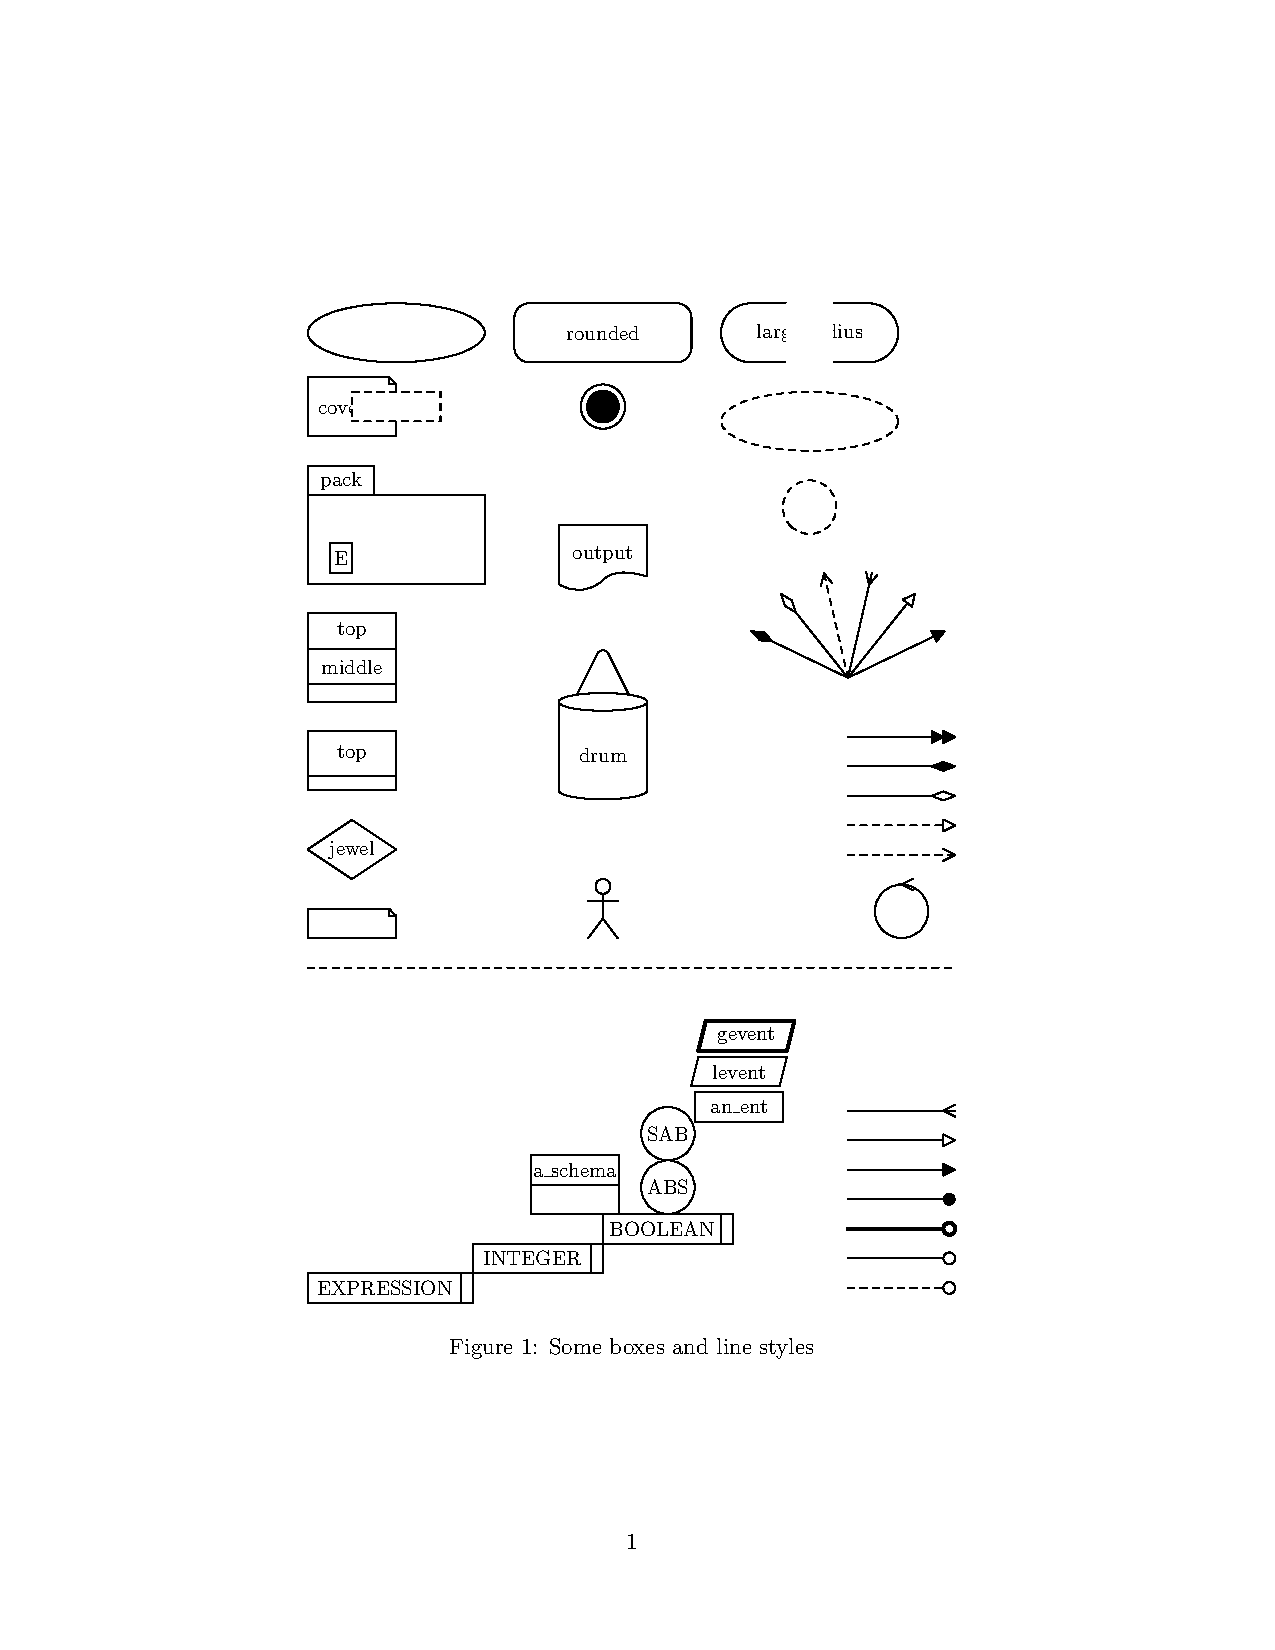
\includegraphics{expeg.1}
\caption{Some boxes and line styles}
\end{figure}

\begin{figure}
\centering
  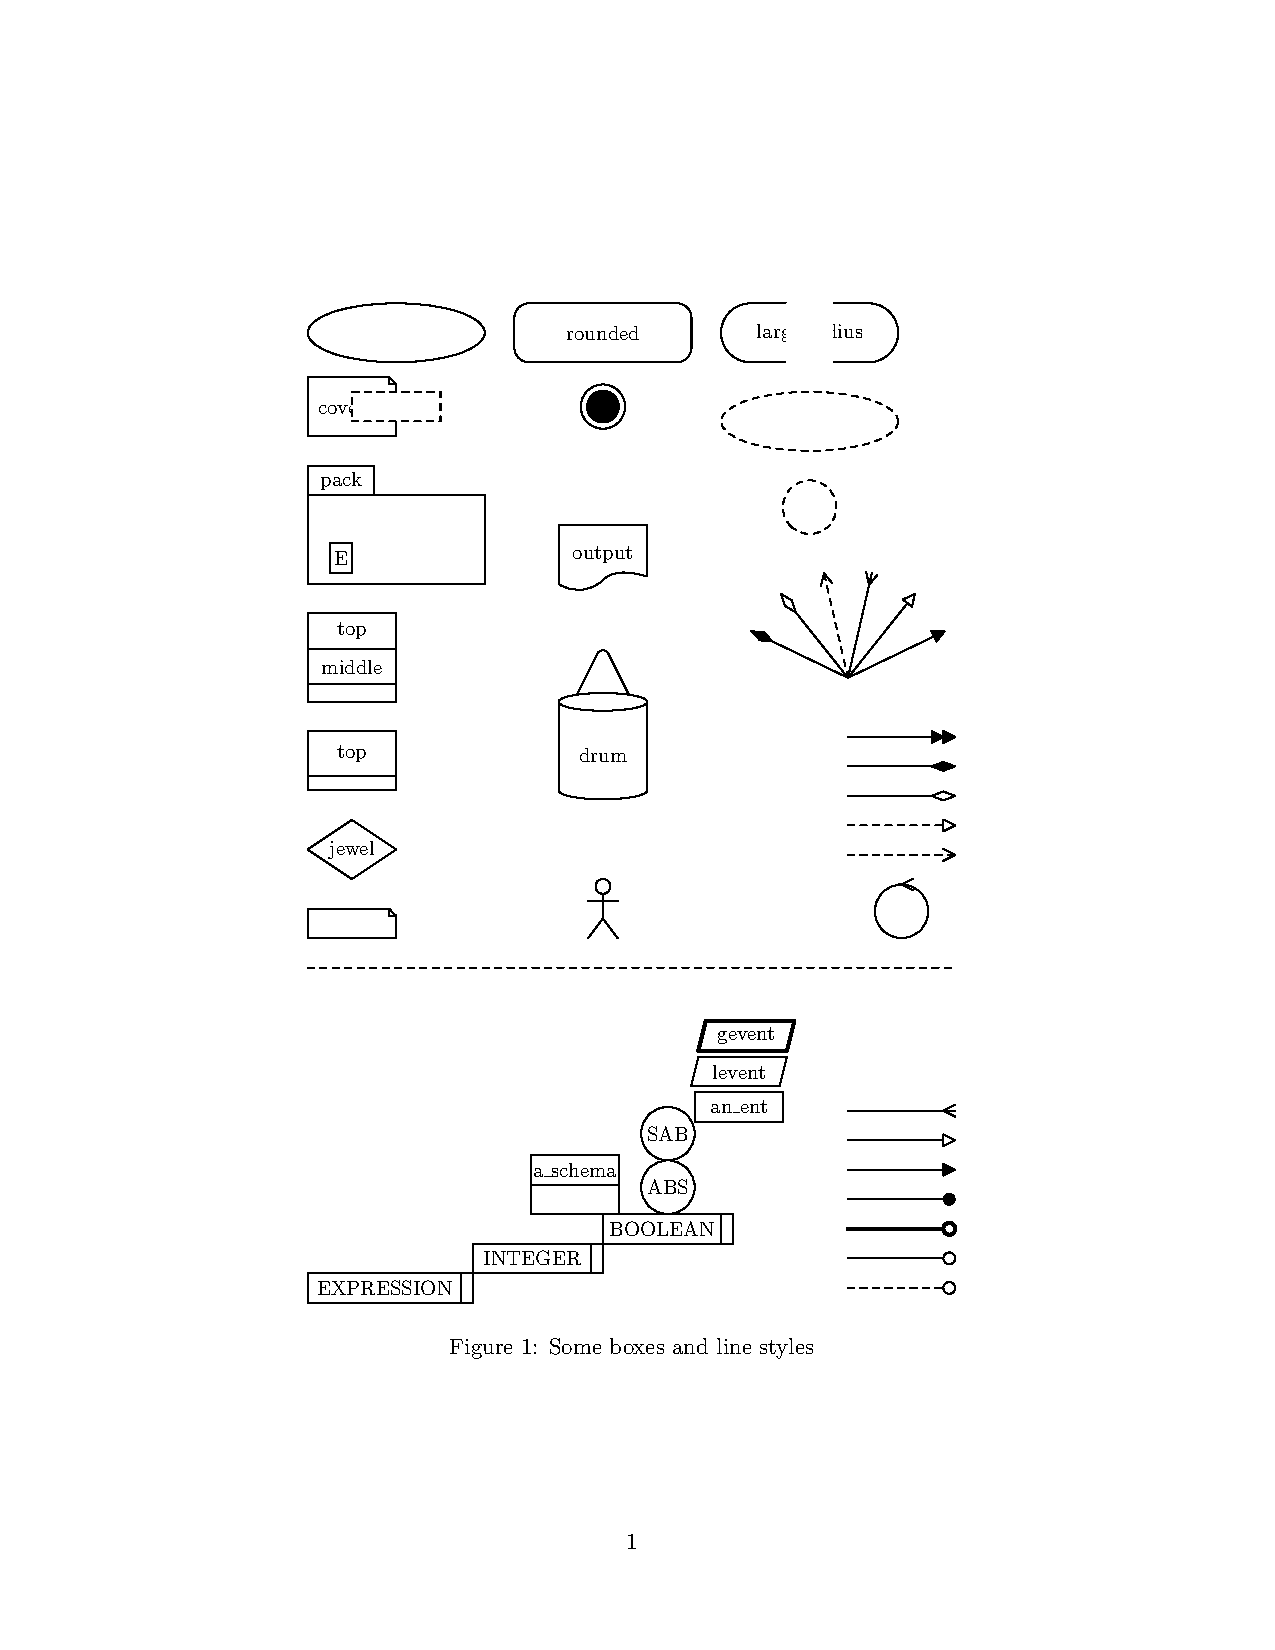
\includegraphics{expeg.2}
\caption{Example schema level diagram}
\end{figure}

\begin{figure}
\centering
  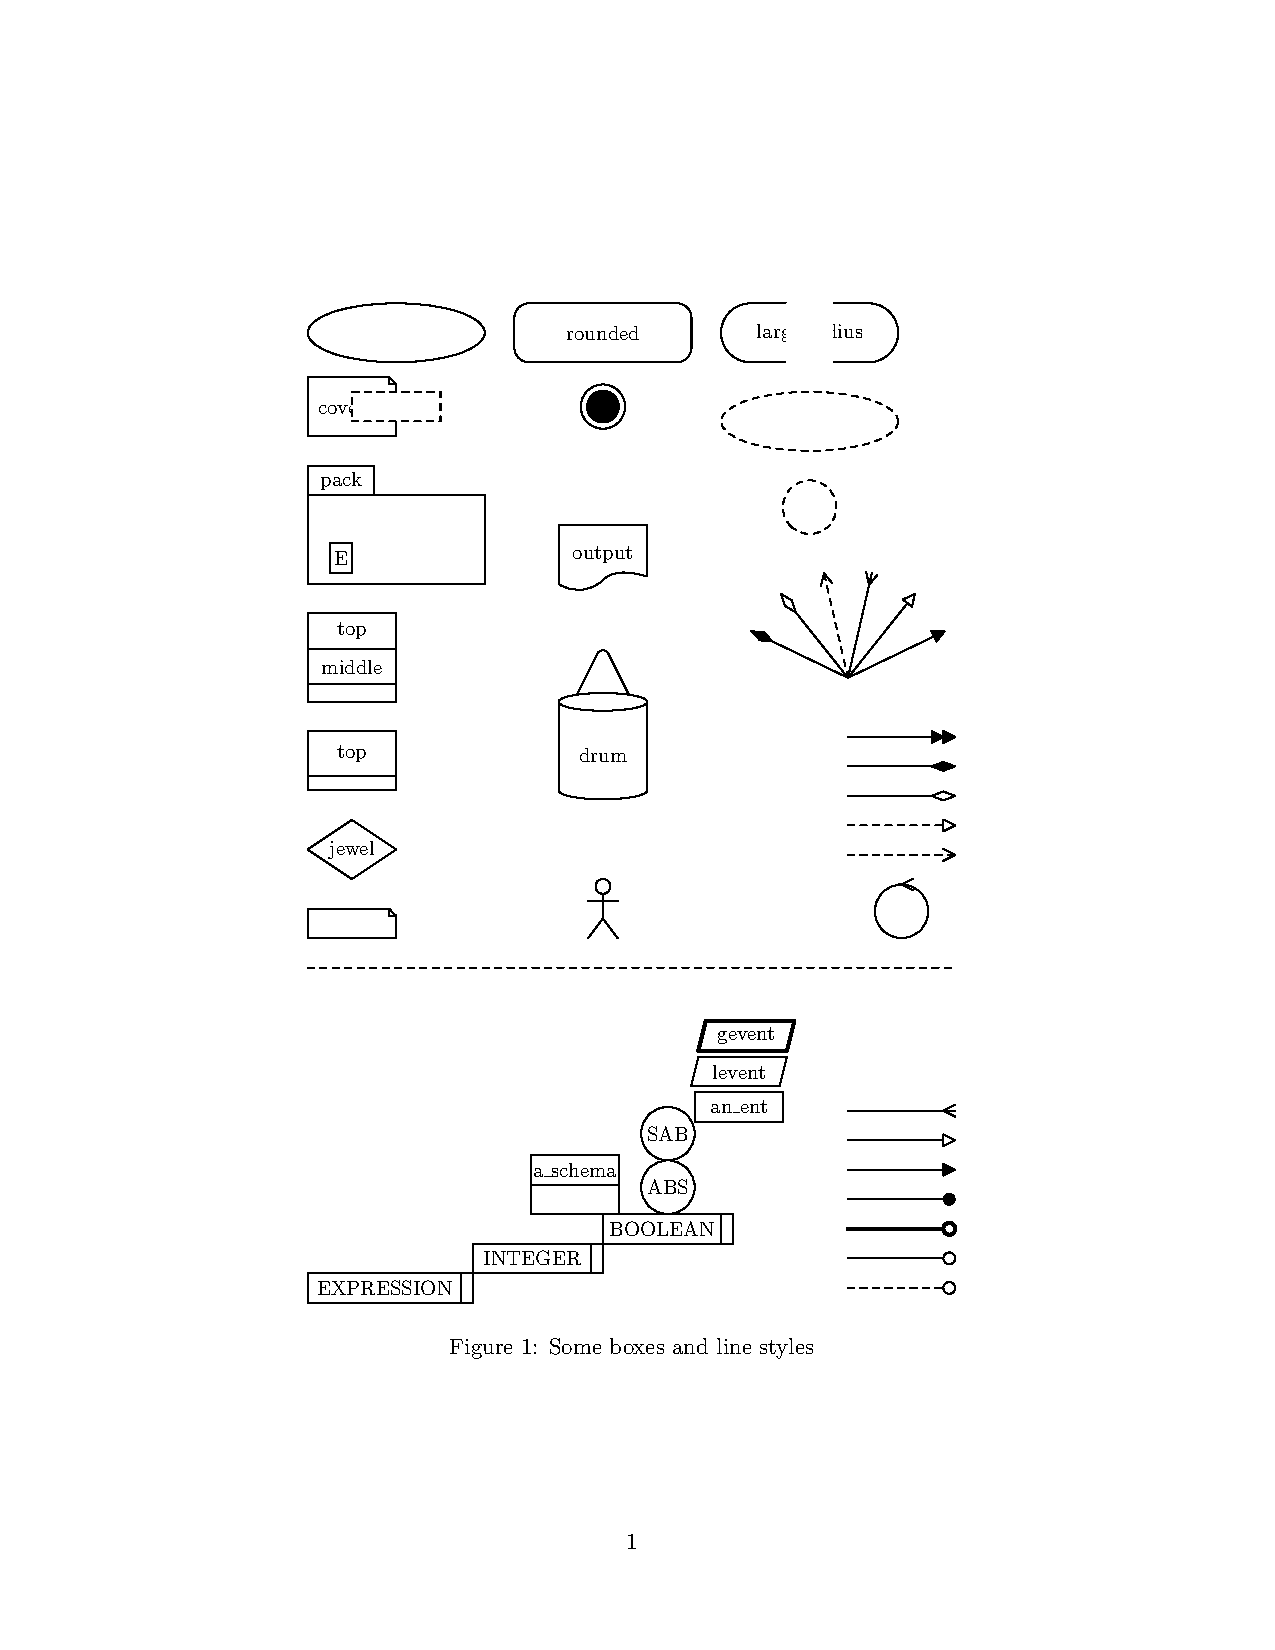
\includegraphics{expeg.3}
\caption{Example diagram of a tree structure}
\end{figure}

\begin{figure}
\centering
  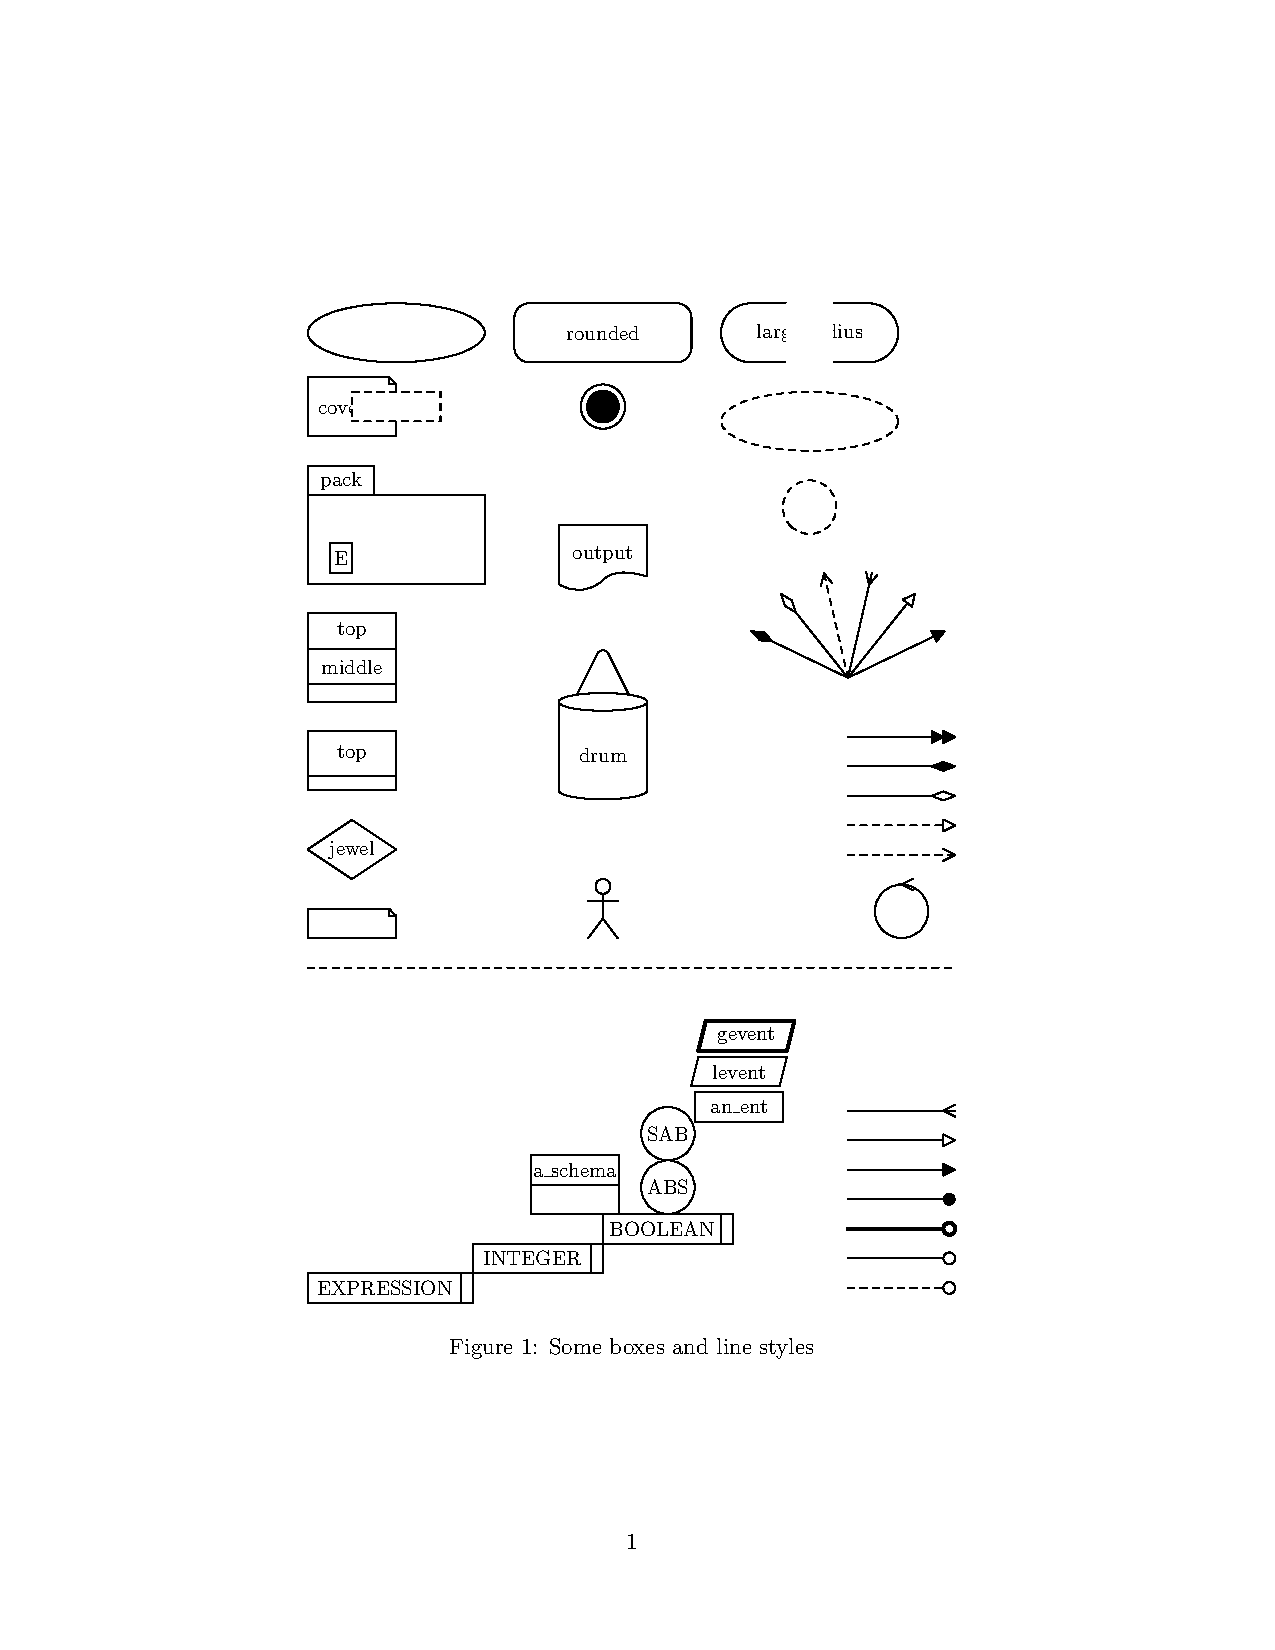
\includegraphics{expeg.4}
\caption{Supertypes and subtypes}
\end{figure}

\begin{figure}
\centering
  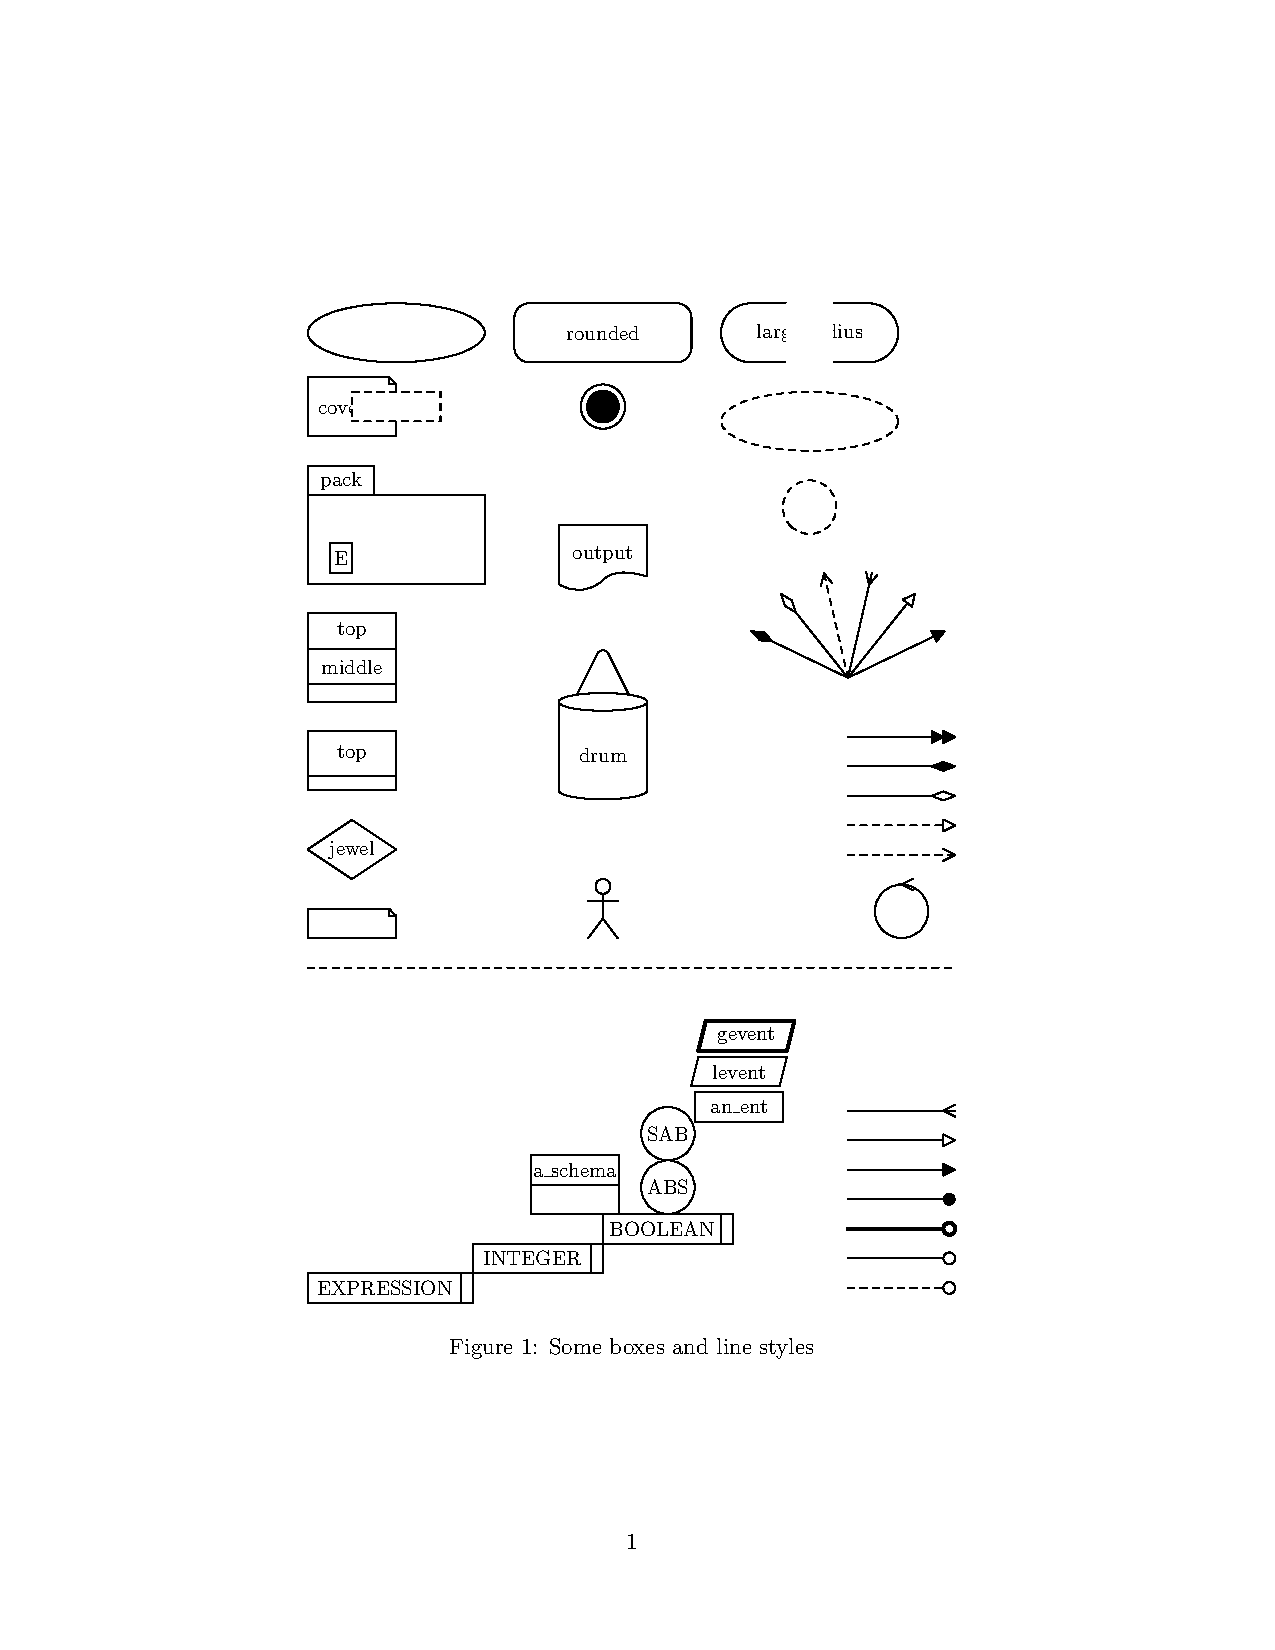
\includegraphics{expeg.5}
\caption{A portion of a large model}
\end{figure}

\begin{figure}
\centering
  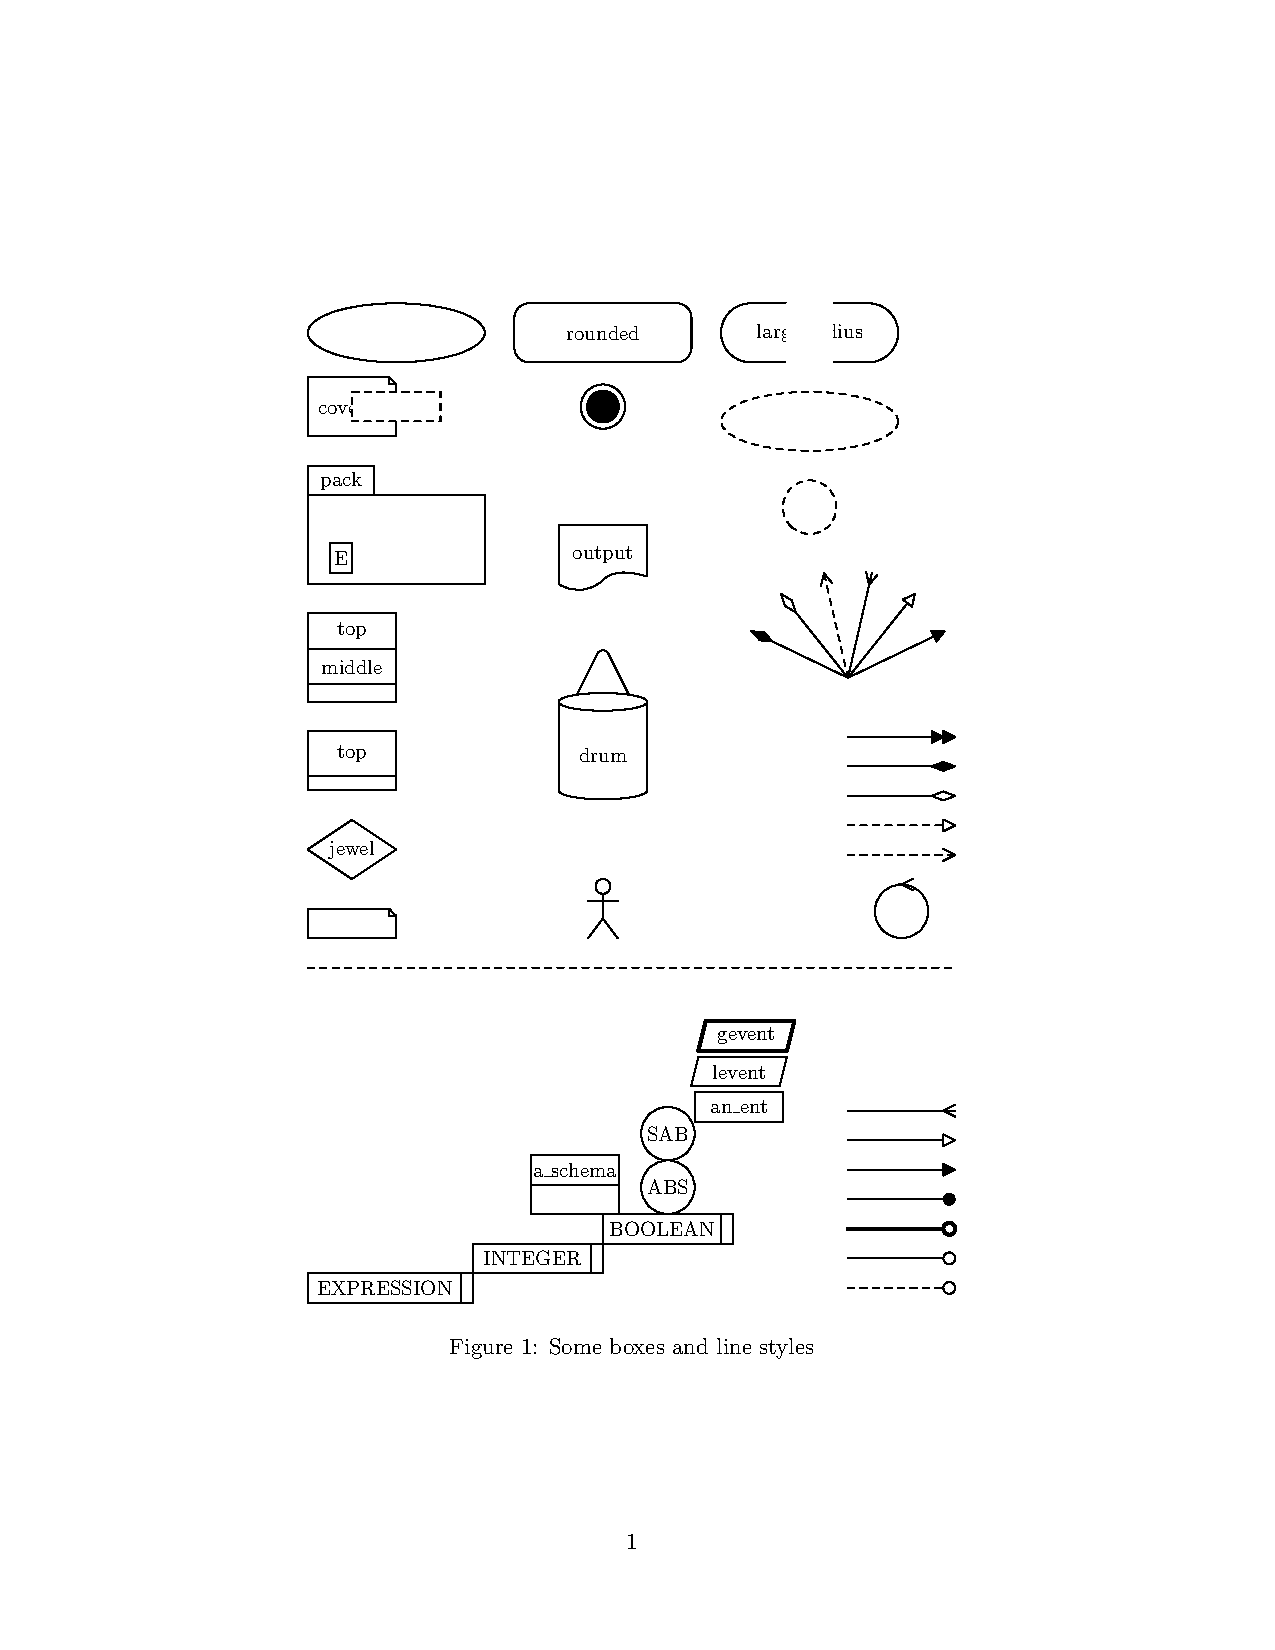
\includegraphics{expeg.6}
\caption{Car model using EXPRESS-G}
\end{figure}

\begin{figure}
\centering
  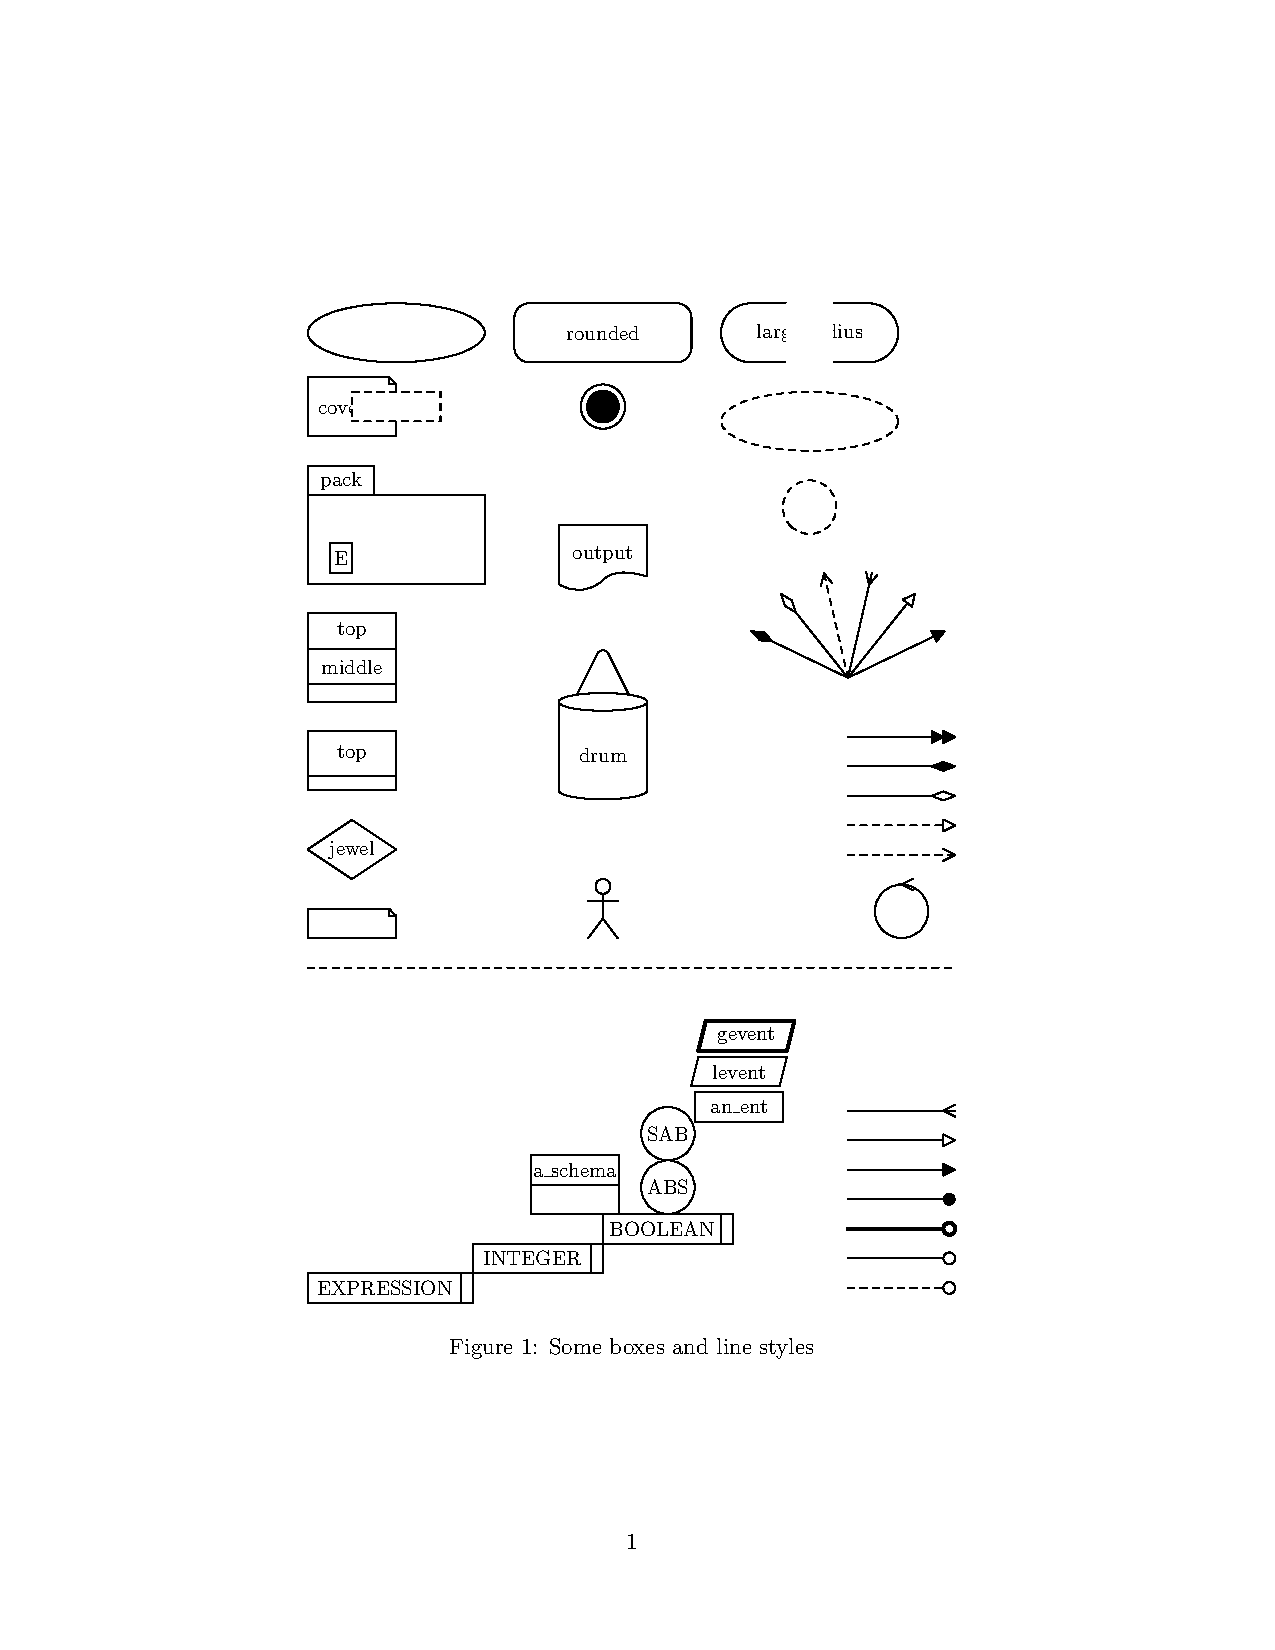
\includegraphics{expeg.7}
\caption{Car model using Shlaer-Mellor}
\end{figure}

\begin{figure}
\centering
  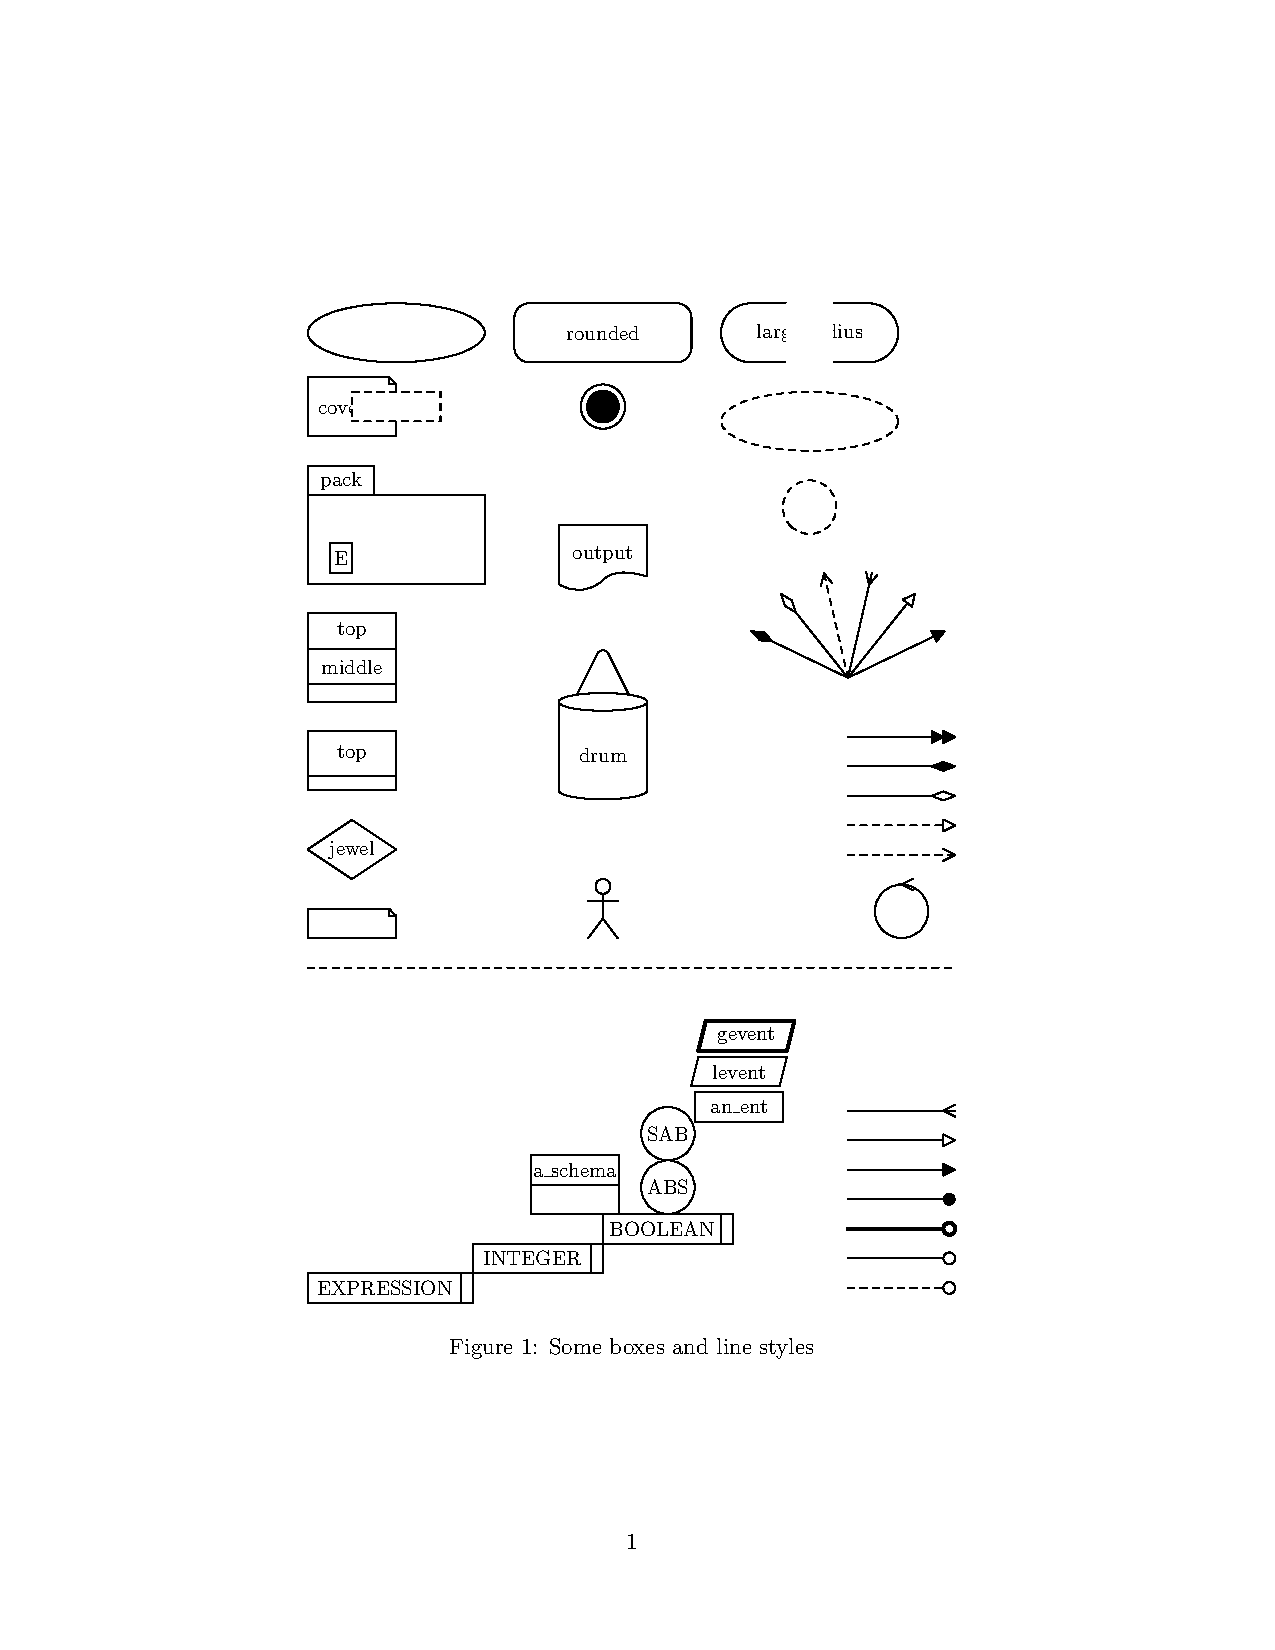
\includegraphics{expeg.8}
\caption{Car model using IDEF1X}
\end{figure}

\begin{figure}
\centering
  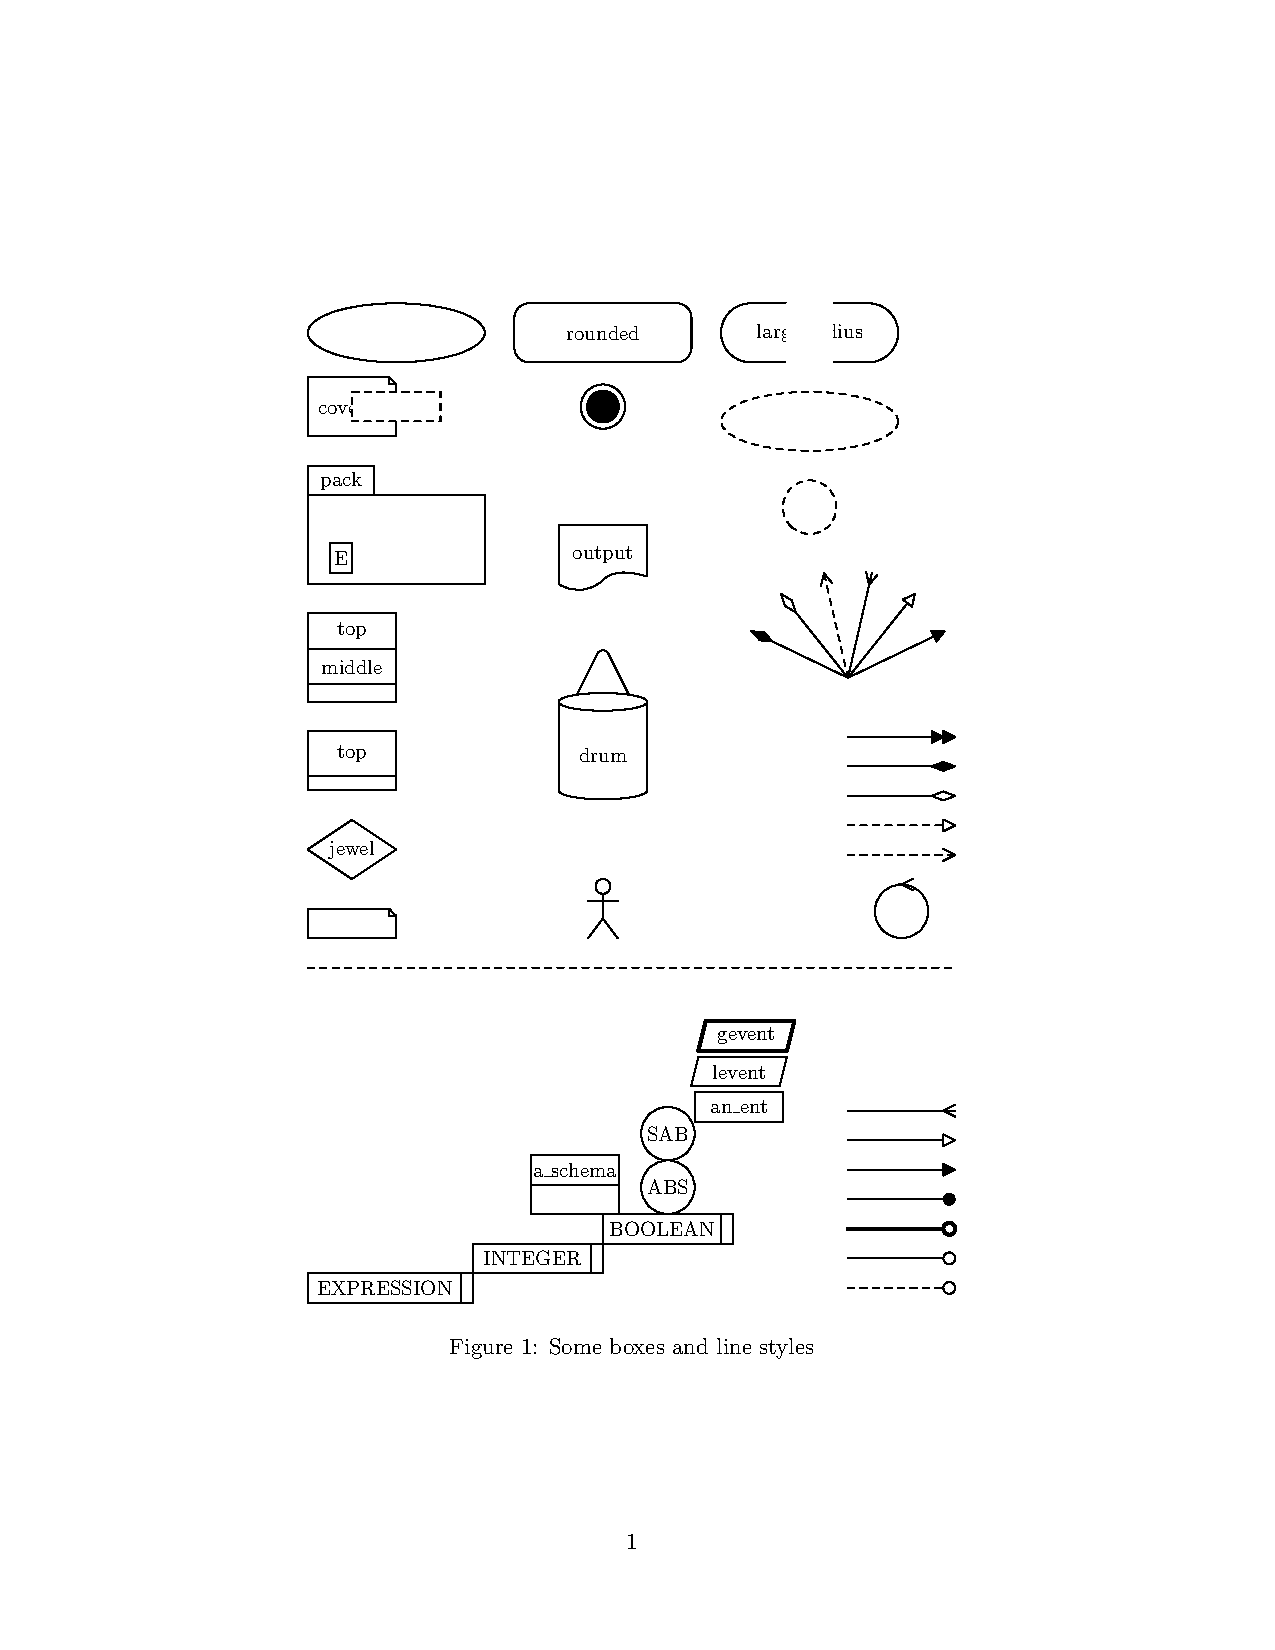
\includegraphics{expeg.9}
\caption{Car model using OMT}
\end{figure}

\begin{figure}
\centering
  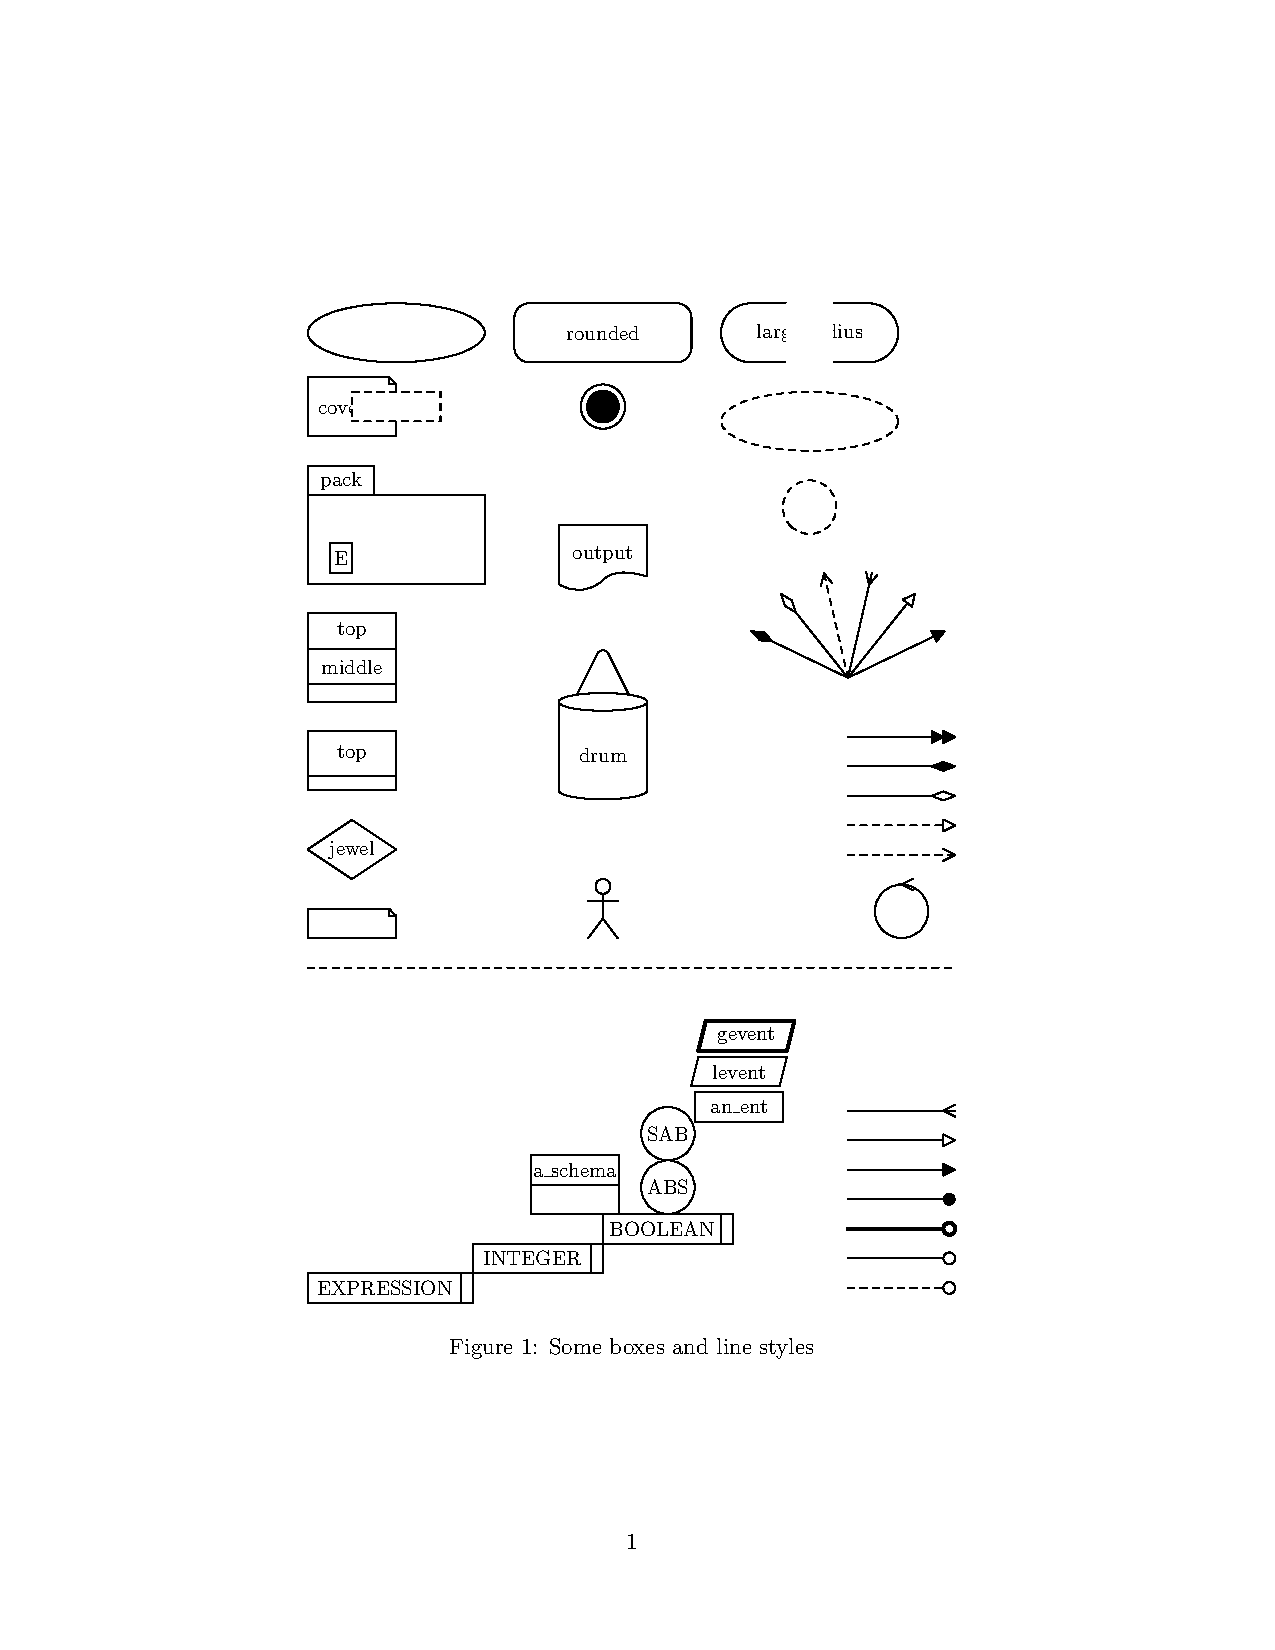
\includegraphics{expeg.10}
\caption{Car model using E-R}
\end{figure}

\begin{figure}
\centering
  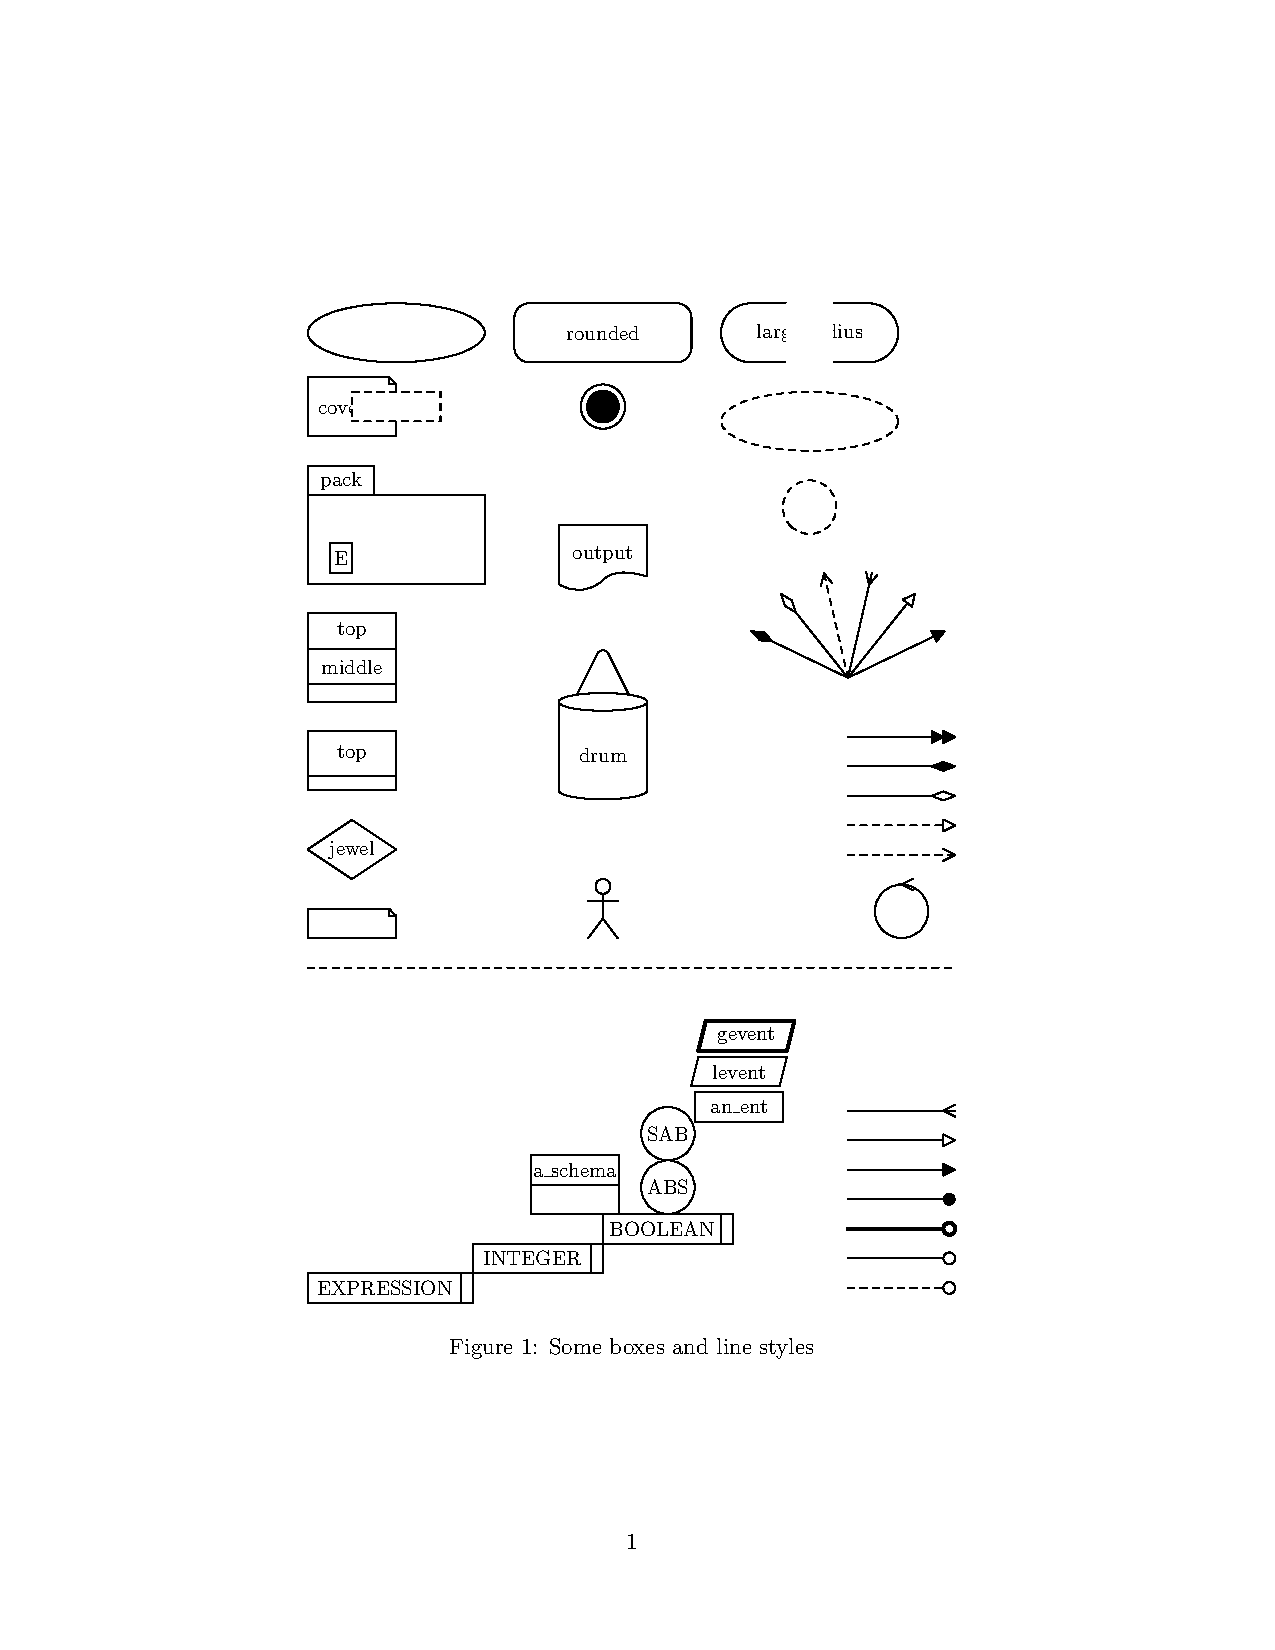
\includegraphics{expeg.11}
\caption{Car model using NIAM}
\end{figure}

\end{document}

%    \end{macrocode}
%
% The end of the \LaTeX{} file.
%    \begin{macrocode}
%</egt>
%    \end{macrocode}
%
% \subsubsection{Using \pdflatex}
%
%    \pdflatex{} generates a \file{.pdf} file directly from \LaTeX{} source
% instead of a \file{.dvi} file. Unfortunately \pdflatex{} does not understand
% \EPS{} in general, but it \emph{does} understand the restricted form
% of \EPS{} generated by \Mpost. By default \pdflatex{} will recognise
% files with an \file{.mps} extension as coming from \Mpost, but \Mpost{}
% generates files with a numeric extension. 
% If you like to use both \Mpost{} and \pdflatex, then it can
% get tedious changing all the numeric extensions to \file{.mps}. The
% following two scripts can help with this. The first is a shell 
% script\footnote{You may well have to modify this to run on your
% operating system.} which calls a Perl script. 
%
% The shell script is called \file{n2mps.sh}. To get suitable versions
% of the example \Mpost{} output files for use with \pdflatex, just do: \\
% |n2mps.sh expeg| \\
% after having run \Mpost{} on \file{expeg.mp}.
%
%    \begin{macrocode}
%<*shell>
#! /bin/sh

#####################################################################
# Shell script n2mps.sh
# Call as: n2mps.sh basename
# List each file basename.* in the directory and run the Perl script
# to copy each basename.N to basenameN.mps, where N is an integer
#
# Copyright 2000, Mauro S. Costa and Peter R. Wilson
#####################################################################

basename=${1:?"A file basename is required."}
extname=N.mps
echo Files $basename.N, where N is a number, will be copied to $basename$extname
for file in `ls $basename.*`
do
 n2mpsprl.prl $file
done

####################### end shell script ###########################

%</shell>
%    \end{macrocode}
% The Perl script, which is called by the \file{n2mps} script:
%    \begin{macrocode}
%<*perl>

#!/usr/local/bin/perl -w

###################################################################
# Perl script: n2mpsprl.prl
# Call as: n2mpsprl.prl filename
# If filename is of the form basename.N, where N is an integer,
# copies file basename.N to file basenameN.mps
#
# Copyright 2000, Mauro S. Costa and Peter R. Wilson
##################################################################

# Test for correct number of input parameters
die "Invalid command line arguments.\nTry $0 <src> \n" if($#ARGV > 1);
die "Invalid command line arguments.\nTry $0 <src> \n" if($#ARGV < 0);

# Assign input file name to variable
$input_file = $ARGV[0];

## test if ends with a number, exit if not
if ($input_file =~ /\w\.\d/) { ; } else { exit; }

# Remove the "dot" from the string variable 
# holding the input file name
$input_file =~ s/\.// ;

# Create a list variable composed of the string variable holding
# the concatenated input file name and the extension ".mps"
@name_list = ($input_file,'.mps') ;

# Join the string variables in the name_list variable into
# a single string variable
$output_file = join("",@name_list) ;

# create a list variable composed to the parameters needed
# for the system copy command excution
@exec_list = ('cp', $ARGV[0], $output_file) ;

# Execute the system copy  ("cp") command
system(@exec_list) ;

############################ end perl script ##########################

%</perl>
%    \end{macrocode}
%
% As an alternative when using \pdflatex{} and the \Lpack{graphicx} package,
% putting \\
% |\DeclareGraphicsRule{*}{mps}{*}{}|    \\
% will cause included graphics files with unknown extensions 
% (e.g., as generated by \Mpost) to be treated as \file{.mps} files.
% \begin{verbatim}
% \documentclass...
% \usepackage{ifpdf}%   you should have this
% \ifpdf
%   \pdfoutput=1
%   \usepackage[pdftex,final]{graphicx}
%   \DeclareGraphicsRule{*}{mps}{*}{}
% \else
%   \usepackage[final]{graphicx}
% \fi
% ...
% \includegraphics{mpfig.23}
% ...
% \end{verbatim}
%
%
% \subsection{Using \LaTeX{} instead of \TeX}
%
%    As already noted, \Mpost{} defaults to using \TeX{} for typesetting
% labels. If you would prefer it to use \LaTeX{} instead, then two things
% have to be done.
% \begin{enumerate}
% \item \Mpost{} looks at the value of an environment variable called |TEX|
%       to see what typesetting system it should use. If the variable is
%       not set, then it uses \TeX. To get it to use \LaTeX{} the environment
%       variable has to be set to |latex|. For example, on the system I use
%       this is done by:
% \begin{verbatim}
% TEX=latex
% export TEX
% \end{verbatim}
%
% \item \LaTeX{} |\documentclass| and |\begin{document}| commands must
%       be put into the |verbatimtex|\ldots|etex| group at the start of
%       the diagramming file. For the example, this might look like
% \begin{verbatim}
% verbatimtex
%   \documentclass{article}
%   % \usepackage{...} % for any packages
%   \def\twolines#1#2{\vbox{\hbox{#1} \hbox{#2}}}
%   \begin{document}
% etex
% \end{verbatim}
%
% \end{enumerate}
%
% \textbf{NOTE:} Both the above are required for \LaTeX. On the other hand,
% if |TEX| is either undefined or has a value other than |tex|, 
% then there must
% be no \LaTeX{} code anywhere in the \file{.mp} file.
%
%    If you need to generate individual self-contained \file{ps} files
% for inclusion in non-\LaTeX{} documents where the font used for labels
% is a member of the Computer Modern family,
% then you need to use LaTeX{} and dvips on \file{*.tex} files that consist
% of only a single diagram and no other text at all. At least on my setup
% I have found it best to run dvips as normal but with output to a file
% instead of a printer. Then use whatever tools are available to you to
% convert the \file{.ps} file to an \file{.eps} one (or at least set the
% correct bounding box values). The primary source on generating and
% using \EPS{} in the \LaTeX{} world is~\cite{RECKDAHL97},
% and~\cite{GOOSSENS97} also has useful information.
%
% \subsection{Using \PS{} fonts}
%
%    \Mpost{} can be made to use \PS{} fonts and, providing the labels
% don't require any special (\TeX) processing, then use of \LaTeX{} may
% be avoided altogether. In order to do this, certain requirements have
% to be put on the content on the \file{.mp} file.
%
% \begin{itemize}
% \item \DescribeVariable{prologues} The 
% diagram file must begin with the line \\
% |prologues:=2;| \\
% which will add a prologue for \PS{} font to the output file.
%
% \item \DescribeVariable{defaultfont} The 
% |defaultfont| must be changed. What it has to be changed
% to depends on the font you want to use. For example, to use the
% Times Roman font, put: \\
% |defaultfont:="ptmr8r";| \\
% just after the |prologues| line.
%
%    For this incantation to work, the file \file{ptmr8r.tfm} must exist
% in a location where \Mpost{} looks for \file{.tfm} files (on the system
% I use it is in directory \texttt{../texmf/fonts/tfm/adobe/times}). Also,
% the file \file{psfonts.map} must include a line like \\
% |ptmr8r  Times-Roman ...| \\
% Again, on my system \file{psfonts.map} is in directory 
% \texttt{../texmf/dvips/misc}.
%
%    I don't know whether or not this works if you don't have a \LaTeX{}
% distribution --- it probably doesn't. But it's unlikely that you don't 
% have one if you
% intend to use \Mpost.
%
% \end{itemize}
%     
%     As a final note on changing fonts, the \Mpost{} |defaultfont| and
% |defaultscale| values only apply to quoted text 
% (e.g., \texttt{"quoted text"}) and not to `btexed' text 
% (e.g., \texttt{btex btexed text etex}). Conversely, \TeX{} or \LaTeX{}
% commands only apply to btexed text and not to quoted text. For more
% details on this, see~\cite{METAFP}.
%    
%
%
%
% \section{The \Mpost{} code} \label{sec:mf}
%
%
%    We start by announcing what it is for.
%
%    \begin{macrocode}
%<*up>
%%% EXPRESSG.MP  MetaPost macros for EXPRESS-G and other BLA diagrams
%%% version 1.5, 31 July 2003
%%% version 1.6, 29 February 2004
%%% version 1.61, 17 March 2004

show "expressg.mp version 1.61, 2004/03/17";

%    \end{macrocode}
%
% \subsection{Variables}
%
% \begin{variable}{u}
%    The unit of length.
%    \begin{macrocode}
newinternal u; numeric u;
u := 1mm;

%    \end{macrocode}
% \end{variable}
%
% \begin{variable}{maxx}
% \begin{variable}{maxy}
%    The maximum x and y coordinates for a diagram.
%    \begin{macrocode}
newinternal maxx, maxy;
numeric maxx, maxy;
maxx := 159.5u;        % smidgeon under 160mm for ISO
maxy := 210u;          % 210mm for ISO

%    \end{macrocode}
% \end{variable}
% \end{variable}
%
% \begin{variable}{defaultdotdiam}
% \begin{variable}{dotdiam}
%    The default and actual diameter of circle and dot line end styles.
%    \begin{macrocode}
newinternal defaultdotdiam, dotdiam;
numeric defaultdotdiam, dotdiam;   
defaultdotdiam := 2u;
dotdiam := defaultdotdiam;

%    \end{macrocode}
% \end{variable}
% \end{variable}
%
% \begin{variable}{normalpensize}
% \begin{variable}{normalpensize}
% \begin{variable}{normalpensize}
% The diameters of the pens for drawing normal, thick and thin lines. (The
% size of the default \Mpost{} pen is 0.5bp).
%    \begin{macrocode}
newinternal normalpensize, thickpensize, thinpensize;
numeric normalpensize, thickpensize, thinpensize;
normalpensize := 0.5bp;
thickpensize  := 1.5bp;
thinpensize   := 0.25bp;
%    \end{macrocode}
% \end{variable}
% \end{variable}
% \end{variable}
%
% \begin{variable}{dotsscale}
% |dotsscale| is the amount the |...pensize| has to be increased so that a 
% dotted line looks as thick as a continuous or dashed line.
%    \begin{macrocode}
newinternal dotsscale; numeric dotsscale;
dotsscale := 2;

%    \end{macrocode}
% \end{variable}
%
% \begin{variable}{normalpen}
% \begin{variable}{thickpen}
% \begin{variable}{thinpen}
% \begin{variable}{dotspen}
% \begin{variable}{dotpen}
%  The pens for drawing lines, plus |dotpen| for drawing a dot line end style.
%    \begin{macrocode}
newinternal normalpen, thickpen, thinpen, dotspen, dotpen;
pen normalpen, thickpen, thinpen, dotspen, dotpen;
normalpen := pencircle scaled normalpensize; % i.e. defaultpen;
thickpen  := pencircle scaled thickpensize;
thinpen   := pencircle scaled thinpensize;
dotspen   := pencircle scaled (dotsscale*normalpensize);
dotpen    := pencircle scaled dotdiam;

%    \end{macrocode}
% \end{variable}
% \end{variable}
% \end{variable}
% \end{variable}
% \end{variable}
%
% \begin{variable}{defaultsmoothrad}
% \begin{variable}{smoothrad}
% The default and initial values for the radius of the arc used for joining
% two lines.
% \changes{v1.3}{2000/05/22}{Added defaultsmoothrad and smoothrad variables}
%    \begin{macrocode}
newinternal defaultsmoothrad;
numeric smoothrad, defaultsmoothrad;
smoothrad := defaultsmoothrad := 2u;

%    \end{macrocode}
% \end{variable}
% \end{variable}
%
% \begin{variable}{defaultdrumlid}
% \begin{variable}{drumlid}
% The default and initial values for the ratio of the minor to major
% diameter of ellipses for the top and bottom of drums.
% \changes{v1.3}{2000/05/22}{Added defaultdrumlid and drumlid variables}
%    \begin{macrocode}
newinternal defaultdrumlid;
numeric drumlid, defaultdrumlid;
drumlid := defaultdrumlid := 0.2;

%    \end{macrocode}
% \end{variable}
% \end{variable}
%
% \begin{variable}{defaultgal}
% \begin{variable}{defaultgab}
% \begin{variable}{defaultgfl}
% \begin{variable}{defaultgfb}
% The default values for the length and base width width of arrowheads and fanins.
%
%    \begin{macrocode}
%%% default length and base width for arrowheads and fanin
newinternal defaultgal, defaultgab, defaultgfl, defaultgfb; 
numeric defaultgal, defaultgab, defaultgfl, defaultgfb; 
defaultgal := defaultgfl := defaultdotdiam;
defaultgab := defaultgfb := defaultgal;

%    \end{macrocode}
% \end{variable}
% \end{variable}
% \end{variable}
% \end{variable}
%
% \begin{variable}{gal}
% \begin{variable}{gab}
% \begin{variable}{gfl}
% \begin{variable}{gfb}
% Values of length and base width of arrowheads and fanins.
%    \begin{macrocode}
%%% length and base width of arrowheads and fanins
newinternal gal, gab, gfl, gfb;  
numeric gal, gab, gfl, gfb;  
gal := defaultgal;
gab := defaultgab;
gfl := defaultgfl;
gfb := defaultgfb;

%    \end{macrocode}
% \end{variable}
% \end{variable}
% \end{variable}
% \end{variable}
%
% \begin{variable}{onelineh}
% The minimum height of a box that encloses a single line of text. 
%
%    \begin{macrocode}
newinternal onelineh;
numeric onelineh;
onelineh := 5u;

%    \end{macrocode}
% \end{variable}
%
% \begin{variable}{sdtbl}
% \begin{variable}{sdtbh}
% \begin{variable}{sdtbs}
% The length, height and inset for a simple data type box. The length is
% sufficient for the name `BOOLEAN' and the height for one line of text.
%    \begin{macrocode}
%%% length, height & inset for simple data type boxes
newinternal sdtbl, sdtbh, sdtbs;
numeric sdtbl, sdtbh, sdtbs; 
sdtbl := 22u; 
sdtbh := onelineh;  
sdtbs := 2u;  

%    \end{macrocode}
% \end{variable}
% \end{variable}
% \end{variable}
%
% \begin{variable}{sdtbel}
% \begin{variable}{sdtbeh}
% \begin{variable}{sdtbes}
% The length, height and inset for a simple EXPRESSION data type box. 
% The length is
% sufficient for the name `EXPRESSION' and the height for one line of text.
%    \begin{macrocode}
%%% length, height & inset for EXPRESSION data type boxes
newinternal sdtbel, sdtbeh, sdtbes; 
numeric sdtbel, sdtbeh, sdtbes; 
sdtbel := 28u;
sdtbeh := sdtbh; sdtbes := sdtbs;

%    \end{macrocode}
% \end{variable}
% \end{variable}
% \end{variable}
%
% \begin{variable}{sdtbgel}
% \begin{variable}{sdtbgeh}
% \begin{variable}{sdtbges}
% The length, height and inset for a simple GENERICENT data type box. 
% The length is
% sufficient for the name `GENERIC\_ENTITY' and the height for one line of text.
% \changes{v1.5}{2003/07/31}{Added sdtbgel, sdtbgeh and sdtbges box lengths}
%    \begin{macrocode}
%%% length, height & inset for GENERICENT data type boxes
newinternal sdtbgel, sdtbgeh, sdtbges; 
numeric sdtbgel, sdtbgeh, sdtbges; 
sdtbgel := 38u;
sdtbgeh := sdtbh; sdtbges := sdtbs;

%    \end{macrocode}
% \end{variable}
% \end{variable}
% \end{variable}
%
% \begin{variable}{pconl}
% The average length of a numeric page connector (e.g., for |9,9 (9,9)|).
%    \begin{macrocode}
%%% average length of numeric page connector
newinternal pconl;
numeric pconl; % length of page connector (for e.g., 9,9 (9,9) )
pconl:=15u;
%    \end{macrocode}
% \end{variable}
%
% \begin{variable}{pconh}
% Height of average page connector (one line of text).
%    \begin{macrocode}
%%% height of page connectors (one line)
newinternal pconh;
numeric pconh; 
pconh := onelineh; 

%    \end{macrocode}
% \end{variable}
%
% \begin{variable}{enth}
% \begin{variable}{typeh}
% The height of a one line ENT(ITY) box (|enth|) and the height of a
% one line ENUM(ERATION), SELECT or TYPE box.
%
%    \begin{macrocode}
%%% heights of entity, enum, select, type boxes (One text line)
newinternal enth, typeh;
numeric enth, typeh; 
enth := onelineh;
typeh := onelineh;

%    \end{macrocode}
% \end{variable}
% \end{variable}
%
% \begin{variable}{ish}
% \begin{variable}{isrh}
% The height of a normal one line interschema box (|ish|) and an
% interschema box with one line each for the name and rename (|isrh|).
%    \begin{macrocode}
%%% height of interschema boxes (one text line, no rename), and (name + rename)
newinternal ish, isrh;
numeric ish, isrh;   
ish  := 2onelineh;
isrh := 3onelineh;

%    \end{macrocode}
% \end{variable}
% \end{variable}
%
% \begin{variable}{schemah}
% Height of a one line SCHEMA box.
%    \begin{macrocode}
%%% height of schema boxes (one text line)
newinternal schemah;
numeric schemah; 
schemah := 2onelineh;

%    \end{macrocode}
% \end{variable}
% 
% \begin{variable}{eventh}
% \begin{variable}{eventslope}
% The height (|eventh|) of a one line (G/L)EVENT box and the slope of the 
% sides of a (G/L)EVENT box.
%    \begin{macrocode}
%%% height and slope of event boxes
newinternal eventh, eventslope;
numeric eventh, eventslope; 
eventh := onelineh;
eventslope := 0.25;

%    \end{macrocode}
% \end{variable}
% \end{variable}
%
% \begin{variable}{nextra}
% \begin{variable}{niextra}
% Margins for namespaces in normal (|nextra|) and inset (|niextra|) boxes.
% Inset boxes are the ENUM, SELECT and TYPE boxes.
%    \begin{macrocode}
%%% extra namespaces for boxed names
newinternal nextra, niextra; 
numeric nextra, niextra; 
nextra := 2u;
niextra := nextra+sdtbs;

%    \end{macrocode}
% \end{variable}
% \end{variable}
%
% \begin{variable}{ndextra}
% Margin for namespace on a relationship line.
%    \begin{macrocode}
%%% extra namespace for attribute names
newinternal ndextra;
numeric ndextra;   
ndextra := nextra+dotdiam;

%    \end{macrocode}
% \end{variable}
%
% \subsection{Utility routines}
%
% \begin{routine}{VH}
% \changes{v1.1}{1999/10/30}{Added VH routine}
% Calculates the intersection point |z$vh| between the vertical line through
% |z$| and the horizontal line through |z$$| (see \fref{fig:vhvh}).
%    \begin{macrocode}
%%% calculates mid-point on a path like |_ (vertical, horizontal)
%%% final points are: z$, z$vh, z$$, where z$vh=(x$,y$$)
def VH(suffix $, $$) = 
  z$vh=(x$,y$$); 
enddef;

%    \end{macrocode}
% \end{routine}
%
% \begin{routine}{VhV}
% \changes{v1.1}{1999/10/30}{Added VhV routine}
% Calculates the point |z$vhv| on the vertical line through |z$| and the
% point |z$$vhv| on the vertical line through |z$$|, such that the line
% |z$vhv--z$$vhv| is horizontal and centered vertically between the given
% points (see \fref{fig:vhvh}).
%    \begin{macrocode}
%%% Calculates mid-points on a path like |_ 
%%%                                        |  (vertical, horizontal, vertical)
%%% final points are: z$, z$vhv, z$$vhv, z$$
def VhV(suffix $, $$) =
  y$$vhv=1/2[y$,y$$]; x$$vhv=x$$;
  z$vhv=(x$,y$$vhv);
enddef;

%    \end{macrocode}
% \end{routine}
%
% \begin{routine}{HvH}
% \changes{v1.1}{1999/10/30}{Added HvH routine}
% Calculates the point |z$hvh| on the horizontal line through |z$| and the
% point |z$$hvh| on the horizontal line through |z$$|, such that the line
% |z$hvh--z$$hvh| is vertical and centered horizontally between the given
% points (see \fref{fig:vhvh}).
%    \begin{macrocode}
%%% Calculates mid-points on a path like -|_ (horizontal, vertical, horizontal)
%%% final points are: z$, z$hvh, z$$hvh, z$$
def HvH(suffix $, $$) =
  x$hvh=1/2[x$,x$$]; y$hvh=y$;
  z$$hvh=(x$hvh,y$$);
enddef;

%    \end{macrocode}
% \end{routine}
%
% \begin{routine}{VyV}
% \changes{v1.1}{1999/10/30}{Added VyV routine}
% A generalisation of |VhV|.
% Calculates the point |z$vyv| on the vertical line through |z$| and the
% horizontal line through |y@|, and the point |z$$vyv| on the vertical 
% line through |z$$| and the horizontal line through |y@| (see \fref{fig:vyxh}).
%    \begin{macrocode}
%%% Calculates turning points on a U shaped path (vertical, horizontal, vertical)
%%% final points are: z$, z$vyv, z$$vyv, z$$
def VyV(suffix $, @, $$) =
  z$$vyv=(x$$,y@);
  z$vyv =(x$, y@);
enddef;

%    \end{macrocode}
% \end{routine}
%
% \begin{routine}{HxH}
% \changes{v1.1}{1999/10/30}{Added HxH routine}
% A generalisation of |HvH|.
% Calculates the point |z$hxh| on the horizontal line through |z$| and the
% vertical line through |x@|, and the 
% point |z$$hgh| on the horizontal line through |z$$| and the vertical
% line through |x@| (see \fref{fig:vyxh}).
%    \begin{macrocode}
%%% Calculates corner points rotated U shaped path (horizontal, vertical, horizontal)
%%% final points are: z$, z$hxh, z$$hxh, z$$
def HxH(suffix $, @, $$) =
  z$$hxh=(x@,y$$);
  z$hxh =(x@,y$);
enddef;

%    \end{macrocode}
% \end{routine}
%
% \begin{routine}{namespace}
% |namespace(|\meta{name}|)(|\meta{margin}|)| calculates the length of
% the text string \meta{name} plus the \meta{margin} length. The
% body is enclosed in parentheses\footnote{Requested by Stephan Hennig, 
% \texttt{ctt} thread \textit{[MP, expressg, latexmp] namespace and textext},
% 16 March 2004} 
% so you can do \verb?c=2namespace...?
% \changes{v1.61}{2004/03/17}{Added parentheses to namespace macro}
%    \begin{macrocode}
%%% calculates length taken up by typesetting str, plus margin 
def namespace(text str)(expr margin) =
  (xpart lrcorner(str) - xpart llcorner(str) + margin)
enddef;

%    \end{macrocode}
% \end{routine}
%
% \begin{routine}{dashes}
% Shorthand for a dashed line style. Use as: |draw ... dashes;|.
%    \begin{macrocode}
def dashes = 
  dashed evenly
enddef;

%    \end{macrocode}
% \end{routine}
%
% \begin{routine}{dots}
% Shorthand for a dotted line style. Use as: |draw ... dots;|.
%    \begin{macrocode}
def dots =
  dashed withdots
enddef;

%    \end{macrocode}
% \end{routine}
%
% \begin{routine}{dashedgrid}
% |dashedgrid(|\meta{nx}, \meta{ny}, \meta{dist}|)| draws a thin dashed grid
% with \meta{nx} and \meta{ny} divisions in the $x$ and $y$ directions,
% with \meta{dist} between the grid lines. The grid lines are numbered.
%    \begin{macrocode}
% draw a general dashed grid
def dashedgrid(expr nx, ny, dist) =
  save zg_, zg__, oldpen;
  pair zg_[], zg__[];
  pen oldpen; oldpen = currentpen;
  pickup thinpen;
  for i = 0 upto nx:
    zg_[i] = (i*dist, 0); zg_[i+1000] = (i*dist, ny*dist);
    draw zg_[i]--zg_[i+1000] dashes;
    label.bot(decimal(i), zg_[i]);
  endfor
  for i = 0 upto ny:
    zg__[i] = (0, i*dist); zg__[i+1000] = (nx*dist, i*dist);
    draw zg__[i]--zg__[i+1000] dashes;
    label.lft(decimal(i), zg__[i]);
  endfor
  pickup oldpen;
enddef; 

%    \end{macrocode}
% \end{routine}
%
% \begin{routine}{drawgrid}
% |drawgrid| draws a thin dashed grid filling the permitted space for an
% ISO Standard diagram. The units are in mm and the lines are at 10mm intervals
% with labeling in terms of mm.
%    \begin{macrocode}
%%% draw a 1cm spaced grid of 16(x) by 21(y) cms. (units are mm)
def drawgrid =
  dashedgrid(16, 21, 10mm);
enddef;

%    \end{macrocode}
% \end{routine}
%
% The box drawing routines take as an argument the suffix (|$|) of the 
% left-hand bottom corner point of the box, and normally the length and
% height of the box. 
% The coordinates of the box corners
% are calculated (|z$bl|, |z$br|, |z$tr| and |z$tl|). The midpoints of
% the sides of the box (|z$bm|, |z$mr|, |z$tm|, |z$ml|) are calculated
% as well. The text `center' of the box is |z$c|, while the geometric
% center of the box will be at the intersection point of the lines
% |z$bm--z$tm| and |z$ml--z$mr|. See \fref{fig:boxpoints} for an 
% illustration.
%
% \begin{routine}{rectpoints}
% \changes{v1.1}{1999/10/30}{Added rectpoints routine}
% The routine |rectpoints($, l, h)| calculates
% the corner and midpoints of a rectangular box with bottom left
% at |z$|, length |l| and height |h|. Note that it does \emph{not}
% calculate the center point (see \fref{fig:boxpoints}).
%    \begin{macrocode}
%%% calculates corner and midpoints of a rectangle, 
%%% bottom left at $, length l, height h
def rectpoints(suffix $)(expr l, h) =
  z$bl = z$; 
  z$tr = (x$+l, y$+h);
  z$br = (x$tr, y$bl);
  z$tl = (x$bl, y$tr);
  z$ml = 1/2[z$bl, z$tl];
  z$mr = 1/2[z$br, z$tr];
  z$bm = 1/2[z$bl, z$br];
  z$tm = 1/2[z$tl, z$tr];
enddef;

%    \end{macrocode}
% \end{routine}
%
% \begin{routine}{rhompoints}
% \changes{v1.1}{1999/10/30}{Added rhompoints routine}
% The routine |rhompoints($, l, h, s)| calculates the corner and midpoints
% of a rhomboid length |l|, height |h|, sideslope |s|, and positioned
% with its bottom left hand corner at |z$|. The center point is \emph{not} 
% calculated (see \fref{fig:eventpoints}).
%    \begin{macrocode}
%%% calculate corner, midpoints and center point of a rhomboid.
def rhompoints(suffix $)(expr l, h, s) =
  save eshift;
  numeric eshift; eshift = s*h;
  z$bl = z$;
  z$tr = (x$+l+eshift, y$+h);
  z$br = (x$bl+l, y$bl);
  z$tl = (x$bl+eshift, y$tr);
  z$ml = 1/2[z$bl, z$tl];
  z$mr = 1/2[z$br, z$tr];
  z$bm = (1/2[x$ml,x$mr], y$bl);
  z$tm = (x$bm, y$tr);
enddef;

%    \end{macrocode}
% \end{routine}
%
% \begin{routine}{circpoints}
% \changes{v1.1}{1999/10/30}{Added circpoints routine}
% The routine |circpoints($, d)| calculates the `corner' and `midpoints'
% on the circumference of a circle, center |z$| and diameter |d|.
%    \begin{macrocode}
%%% calculate circumferential points on a circle
def circpoints(suffix $)(expr diam) =
  save rad, sinrad, cosrad;
  numeric rad, sinrad, cosrad;
  rad = diam/2;
  sinrad = rad*(sind 45);
  cosrad = rad*(cosd 45);
  z$c=z$;
  z$ml=(x$c-rad, y$c);
  z$mr=(x$c+rad, y$c);
  z$bm=(x$c, y$c-rad);
  z$tm=(x$c, y$c+rad);
  z$tr=(x$c+cosrad, y$c+sinrad);
  z$bl=(x$c-cosrad, y$c-sinrad);
  z$br=(x$tr, y$bl);
  z$tl=(x$bl, y$tr);
enddef;

%    \end{macrocode}
% \end{routine}
%
% \subsection{Path routines}
% \changes{v1.4}{2000/07/10}{Added path routines}
%
% \begin{routine}{~}
% The binary operator |~| is a reimplementation of the METAFONT plain base
% |softjoin| path connector (METAFONTbook, page 266); 
% it connects paths via a small circular arc
% radius |smoothrad|.
%    \begin{macrocode}
%%% circular arc join between two paths
tertiarydef p ~ q =
  begingroup
  c_ := fullcircle scaled 2smoothrad shifted point 0 of q;
  a_ := ypart(c_ intersectiontimes p);
  b_ := ypart(c_ intersectiontimes q);
  if a_ < 0: point 0 of p{direction 0 of p} else: subpath(0,a_) of p fi
    ... if b_ < 0: {direction infinity of q}point infinity of q
        else: subpath(b_,infinity) of q fi
  endgroup
enddef;

%    \end{macrocode}
% \end{routine}
%
% \begin{routine}{sharply}
% |sharply(zi, zj, ...zn)| creates a piecewise linear path through the
% given points. (The code is based on the |flex| routine,
% page 267 of the METAFONTbook).
%    \begin{macrocode}
%%% piecewise linear path between the given points
def sharply(text t) =     % t is a list of pairs
  hide(n_:=0; for z=t: z_[incr n_]:=z; endfor)
  z_1 for k=2 upto n_: --z_[k] endfor
enddef;

%    \end{macrocode}
% \end{routine}
%
% \begin{routine}{smoothly}
% |smoothly(zi, zj, ...zn)| creates a piecewise linear path through the
% given points, with the sharp corners replaced by circular arcs of radius
% |smoothrad|.
% page 267 of the METAFONTbook).
%    \begin{macrocode}
%%% piecewise linear path between the given points with smooth corners
def smoothly(text t) =     % t is a list of pairs
  hide(n_:=0; for z=t: z_[incr n_]:=z; endfor)
  (z_1 for k=2 upto n_-1: --z_[k]) ~ (z_[k] endfor --z_[n_])
enddef;

%    \end{macrocode}
% \end{routine}
%
% \subsection{Line end drawing routines}
%
% \changes{v1.4}{2000/07/10}{Added individual line end drawing routines}
% \begin{routine}{drawO}
% Draw an open circle, diameter |dotdiam| at the end of the vector
% |z$| to |z$$|. Any underlying graphic/text will be hidden.
% All the line end drawing routines have similar code.
%    \begin{macrocode}
%%% Draw an open circle at end of vector from $ to $$ 
def drawO(suffix $, $$) = 
%    \end{macrocode}
% Keep everything inside a group and specify the local variables.
%    \begin{macrocode}
  begingroup
  save v_, c_, l, p;
%    \end{macrocode}
% Specify the types of the local variables.
%    \begin{macrocode}
  pair v_, c_;
  numeric l;
  path p;
%    \end{macrocode}
% |v_| is the difference between the start and end points of the line. 
% That is, it is the vector from the end point to the start point.
%    \begin{macrocode}
  v_ := z$-z$$;
%    \end{macrocode}
% \DescribeRoutine{++}
% \DescribeRoutine{xpart}
% \DescribeRoutine{ypart}
% Using \Mpost's Pythagorean addition operator |++|, where |a++b| means
% $\sqrt{a^{2}+b^{2}}$, we can calculate the length |l| of the line from
% the x and y dimension (|xpart| and |ypart|) of the vector |v_|.
%    \begin{macrocode}
  l := (xpart v_)++(ypart v_);  % length of the line
%    \end{macrocode}
% Using mediation involving the ratio of the circle radius to the length
% of the line, calculate |c_|, the required position of the center of 
% the circle at the end of the line.
%    \begin{macrocode}
  c_ := (dotdiam/(2l))[z$$,z$];
%    \end{macrocode}
% |p| is the path for drawing the circle.
%    \begin{macrocode}
  p := fullcircle scaled dotdiam shifted c_;
%    \end{macrocode}
% Erase anything underneath the circle.
%    \begin{macrocode}
  unfill p;
%    \end{macrocode}
% Now we can draw the circle (twice to make sure it shows).
%    \begin{macrocode}
  draw p; draw p;
%    \end{macrocode}
% Finish the local group and end.
%    \begin{macrocode}
  endgroup
enddef;

%    \end{macrocode}
% \end{routine}
%
% \begin{routine}{drawD}
% Draw a closed circle, diameter |dotdiam| at the end of the vector
% |z$| to |z$$|. Any underlying graphic/text will be hidden.
%    \begin{macrocode}
%%% Draw a closed circle at end of vector from $ to $$ 
def drawD(suffix $, $$) = 
  begingroup
  save v_, c_, l, p;
  pair v_, c_;
  numeric l;
  path p;
  v_ := z$-z$$;
  l := (xpart v_)++(ypart v_);  % length of the line
  c_ := (dotdiam/(2l))[z$$,z$];
  p := fullcircle scaled dotdiam shifted c_;
  fill p;
  endgroup
enddef;

%    \end{macrocode}
% \end{routine}
%
% \begin{routine}{drawOA}
% Draw an open arrowhead, length |gal| and base width |gab|,
% at the end of the vector from |z$| to |z$$|.
% The same general code pattern is used for non-circular
% line end styles, and is described here. It is not too different
% from drawing circular ends, except that the orientation of the line
% has to be taken into account.
%    \begin{macrocode}
%%% draw an open arrowhead at end of vector from $ to $$
def drawOA(suffix $, $$) =
  begingroup
  save v_, c_, v_u, c_t, c_b, l, hb, p;
  pair v_, c_, v_u, c_t, c_b;
  numeric l, hb;
  path p;
  hb := gab/2;
  v_ := z$-z$$;
  l := (xpart v_)++(ypart v_);  % length of the line
  c_ := (gal/(l))[z$$,z$];      % base of arrowhead
%    \end{macrocode}
% Calculate the unit vector in the direction of the line.
%    \begin{macrocode}
  v_u := unitvector v_;
%    \end{macrocode}
% Calculate one of the corner points on the base of the triangle by
% shifting the midbase point in the direction of the normal to the
% line by half the base width.
%    \begin{macrocode}
  c_t := c_ shifted (-hb*(ypart v_u), hb*(xpart v_u));
%    \end{macrocode}
% Specify that the other corner point is symmetrically opposite the first.
%    \begin{macrocode}
  c_b - c_ = c_ - c_t;
%    \end{macrocode}
% Draw the triangular arrowhead.
%    \begin{macrocode}
  p = c_b--z$$--c_t--cycle;
  unfill p;
  draw p; draw p;
  endgroup
enddef;

%    \end{macrocode}
% \end{routine}
%
% \begin{routine}{drawCA}
% Draw a closed (black) arrowhead, length |gal| and base width |gab|,
% at the end of the vector from |z$| to |z$$|.
%    \begin{macrocode}
%%% draw a closed arrowhead at end of vector from $ to $$
def drawCA(suffix $, $$) =
  begingroup
  save v_, c_, v_u, c_t, c_b, l, hb, p;
  pair v_, c_, v_u, c_t, c_b;
  numeric l, hb;
  path p;
  hb := gab/2;
  v_ := z$-z$$;
  l := (xpart v_)++(ypart v_);  % length of the line
  c_ := (gal/(l))[z$$,z$];      % base of arrowhead
  v_u := unitvector v_;
  c_t := c_ shifted (-hb*(ypart v_u), hb*(xpart v_u));
  c_b - c_ = c_ - c_t;
  p = c_b--z$$--c_t--cycle;
  filldraw p;
  endgroup
enddef;

%    \end{macrocode}
% \end{routine}
%
% \begin{routine}{drawA}
% Draw a simple arrowhead, length |gal| and base width |gab|,
% at the end of the vector from |z$| to |z$$|.
%    \begin{macrocode}
%%% draw a simple arrowhead at end of vector from $ to $$
def drawA(suffix $, $$) =
  begingroup
  save v_, c_, v_u, c_t, c_b, l, hb, p;
  pair v_, c_, v_u, c_t, c_b;
  numeric l, hb;
  path p;
  hb := gab/2;
  v_ := z$-z$$;
  l := (xpart v_)++(ypart v_);  % length of the line
  c_ := (gal/(l))[z$$,z$];      % base of arrowhead
  v_u := unitvector v_;
  c_t := c_ shifted (-hb*(ypart v_u), hb*(xpart v_u));
  c_b - c_ = c_ - c_t;
  p = c_b--z$$--c_t;
  draw p;
  endgroup
enddef;

%    \end{macrocode}
% \end{routine}
%
% \begin{routine}{drawF}
% Draw a fanin, length |gfl| and base width |gfb|,
% at the end of the vector from |z$| to |z$$|.
%    \begin{macrocode}
%%% draws a fanin at the end of the vector from $ to $$
def drawF(suffix $, $$) =
  begingroup
  save v_, c_, v_u, c_t, c_b, l, hb, p;
  pair v_, c_, v_u, c_t, c_b;
  numeric l, hb;
  path p;
  hb := gfb/2;
  v_ := z$-z$$;
  l := (xpart v_)++(ypart v_);  % length of the line
  c_ := (gfl/(l))[z$$,z$];      % apex of fan
  v_u := unitvector v_;
  c_t := z$$ shifted (-hb*(ypart v_u), hb*(xpart v_u));
  c_b - z$$ = z$$ - c_t;
  p = c_b--c_--c_t;
  draw p;
  endgroup
enddef;

%    \end{macrocode}
% \end{routine}
%
%
% \subsection{Line drawing routines}
% \changes{v1.4}{2000/07/10}{Stripped in-line line end code from line drawing routines}
%
% \begin{routine}{drawdots}
% Draw a dotted line between the two points |z$| and |z$$|.
%    \begin{macrocode}
%%% Draw a dotted line from $ to $$
def drawdots(suffix $, $$) = 
  pickup dotspen;
  draw z$--z$$ dots; 
  pickup normalpen;
enddef;

%    \end{macrocode}
% \end{routine}
%
% \begin{routine}{drawdotsthree}
% Draw a straight dotted line between the three points |z$|, |z@| and |z$$|.
%    \begin{macrocode}
%%% Draws the dotted line $--@--$$
def drawdotsthree(suffix $, @, $$) = 
  pickup dotspen;
  draw z$--z@--z$$ dots; 
  pickup normalpen;
enddef;

%    \end{macrocode}
% \end{routine}
%
% \begin{routine}{drawdotsfour}
% Draw a straight dotted line between the four points |z$|, |z@|, |z@@| and |z$$|.
%    \begin{macrocode}
%%% Draw the dotted line $--@--@@--$$
def drawdotsfour(suffix $, @, @@, $$) = 
  pickup dotspen;
  draw z$--z@--z@@--z$$ dots; 
  pickup normalpen;
enddef;

%    \end{macrocode}
% \end{routine}
%
% \begin{routine}{drawdotsO}
% Draw a dotted line between the two points |z$| and |z$$|, 
% ending in an open circle, diameter |dotdiam|, at |z$$|. 
%    \begin{macrocode}
%%% Draw a dotted line from $ to $$ with open circle at $$
def drawdotsO(suffix $, $$) = 
  pickup dotspen;
  draw z$--z$$ dots;
  pickup normalpen;
  drawO($, $$);
enddef;

%    \end{macrocode}
% \end{routine}
%
% \begin{routine}{drawdotsthreeO}
% Draw a straight dotted line between the three points |z$|, |z@| and |z$$|,
% ending in an open circle, diameter |dotdiam|, at |z$$|.
%    \begin{macrocode}
%%% Draws the dotted line $--@--$$
def drawdotsthreeO(suffix $, @, $$) = 
  pickup dotspen;
  draw z$--z@--z$$ dots; 
  pickup normalpen;
  drawO(@, $$);
enddef;

%    \end{macrocode}
% \end{routine}
%
% \begin{routine}{drawdotsfourO}
% Draw a straight dotted line between the four points |z$|, |z@|, |z@@| and |z$$|,
% ending in an open circle, diameter |dotdiam|, at |z$$|.
%    \begin{macrocode}
%%% Draw the dotted line $--@--@@--$$
def drawdotsfourO(suffix $, @, @@, $$) = 
  pickup dotspen;
  draw z$--z@--z@@--z$$ dots; 
  pickup normalpen;
  drawO(@@, $$);
enddef;

%    \end{macrocode}
% \end{routine}
%
% \begin{routine}{drawdotsOO}
% Draw a dotted line between the two points |z$| and |z$$|, 
% ending in open circles, diameter |dotdiam|, at |z$| and |z$$|.
%    \begin{macrocode}
%%% Draw the dotted line from $ to $$, ending in circles diameter dotdiam at $ and $$
def drawdotsOO(suffix $, $$) =
  pickup dotspen;
  draw z$--z$$ dots;
  pickup normalpen;
  drawO($, $$); drawO($$, $);
enddef;

%    \end{macrocode}
% \end{routine}
%
% \begin{routine}{drawdash}
% Draw a dashed line between the two points |z$| and |z$$|.
%    \begin{macrocode}
%%% draws a dashed line from $ to $$
def drawdash(suffix $, $$) = 
  draw z$--z$$ dashes; 
enddef;

%    \end{macrocode}
% \end{routine}
%
% \begin{routine}{drawdashthree}
% Draw a straight dashed line between the three points |z$|, |z@| and |z$$|.
%    \begin{macrocode}
%%% draws the dashed line $--@--$$
def drawdashthree(suffix $, @, $$) = 
  draw z$--z@--z$$ dashes; 
enddef;

%    \end{macrocode}
% \end{routine}
%
% \begin{routine}{drawdashfour}
% Draw a straight dashed line between the four points |z$|, |z@|, |z@@| and |z$$|.
%    \begin{macrocode}
%%% draws the dashed line $--@--@@--$$
def drawdashfour(suffix $, @, @@, $$) = 
  draw z$--z@--z@@--z$$ dashes; 
enddef;

%    \end{macrocode}
% \end{routine}
%
% \begin{routine}{drawdashO}
% Draw a dashed line between the two points |z$| and |z$$|, 
% ending in an open circle, diameter |dotdiam|, at |z$$|.
%    \begin{macrocode}
%%% draws a dashed line from $ to $$, ending in a circle diameter dotdiam at $$
def drawdashO(suffix $, $$) =
  draw z$--z$$ dashes;
  drawO($, $$);
enddef;

%    \end{macrocode}
% \end{routine}
%
% \begin{routine}{drawdashthreeO}
% Draw a straight dashed line between the three points |z$|, |z@| and |z$$|, 
% ending in an open circle, diameter |dotdiam|, at |z$$|.
%    \begin{macrocode}
%%% draws the dashed line $--@--$$ with circle at $$
def drawdashthreeO(suffix $, @, $$) =
  draw z$--z@--z$$ dashes;
  drawO(@, $$);
enddef;

%    \end{macrocode}
% \end{routine}
%
% \begin{routine}{drawdashfourO}
% Draw a straight dashed line between the four points |z$|, |z@|, |z@@| and |z$$|, 
% ending in an open circle, diameter |dotdiam|, at |z$$|.
%    \begin{macrocode}
%%% draws the dashed line $--@--@@--$$ with circle at $$
def drawdashfourO(suffix $, @, @@, $$) =
  draw z$--z@--z@@--z$$ dashes;
  drawO(@@, $$);
enddef;

%    \end{macrocode}
% \end{routine}
%
% \begin{routine}{drawdashOO}
% Draw a dashed line between the two points |z$| and |z$$|, 
% ending in open circles, diameter |dotdiam|, at |z$| and |z$$|.
%    \begin{macrocode}
% drawdashOO($, $$)
%%% draws a dashed line from $ to $$, ending in circles diameter dotdiam at $ and $$
def drawdashOO(suffix $, $$) =
  draw z$--z$$ dashes;
  drawO($, $$); drawO($$, $);
enddef;

%    \end{macrocode}
% \end{routine}
%
% \begin{routine}{drawnormal}
% Draw a normal thickness line between the two points |z$| and |z$$|.
%    \begin{macrocode}
%%% draws a normal line from $ to $$.
def drawnormal(suffix $, $$) =
  draw z$--z$$;
enddef;

%    \end{macrocode}
% \end{routine}
%
% \begin{routine}{drawnormalthree}
% Draw a straight normal thickness line between the three points |z$|, |z@| and |z$$|.
%    \begin{macrocode}
% drawnormalthree($, @, $$)
%%% draws the normal line $--@--$$
def drawnormalthree(suffix $, @, $$) = 
  draw z$--z@--z$$; 
enddef;

%    \end{macrocode}
% \end{routine}
%
% \begin{routine}{drawnormalfour}
% Draw a straight normal thickness line between the four points |z$|, |z@|, |z@@| and |z$$|.
%    \begin{macrocode}
%%% draws the normal line $--@--@@--$$
def drawnormalfour(suffix $, @, @@, $$) = 
  draw z$--z@--z@@--z$$; 
enddef;

%    \end{macrocode}
% \end{routine}
%
% \begin{routine}{drawnormalO}
% Draw a straight normal thickness line between the two points |z$| and |z$$|, 
% ending in an open circle, diameter |dotdiam|, at |z$$|.
%    \begin{macrocode}
% drawnormalO($, $$)
%%% draws a normal line from $ to $$, ending in a circle diameter dotdiam at $$
def drawnormalO(suffix $, $$) =
  draw z$--z$$;
  drawO($, $$);
enddef;

%    \end{macrocode}
% \end{routine}
%
% \begin{routine}{drawnormalthreeO}
% Draw a straight normal thickness line between the three points |z$|, |z@| and |z$$|, 
% ending in an open circle, diameter |dotdiam|, at |z$$|.
%    \begin{macrocode}
%%% draws the normal line $--@--$$, ending in a circle at $$
def drawnormalthreeO(suffix $, @, $$) =
  draw z$--z@--z$$;
  drawO(@, $$);
enddef;

%    \end{macrocode}
% \end{routine}
%
% \begin{routine}{drawnormalfourO}
% Draw a straight normal thickness line between the four points |z$|, |z@|, |z@@| and |z$$|, 
% ending in an open circle, diameter |dotdiam|, at |z$$|.
%    \begin{macrocode}
%%% draws the line $--@--@@--$$, ending in a circle at $$
def drawnormalfourO(suffix $, @, @@, $$) =
  draw z$--z@--z@@--z$$;
  drawO(@@, $$);
enddef;


%    \end{macrocode}
% \end{routine}
%
% \begin{routine}{drawnormalOO}
% Draw a straight normal thickness line between the two points |z$| and |z$$|, 
% ending in open circles, diameter |dotdiam|, at |z$| and |z$$|.
%    \begin{macrocode}
% drawnormalOO($, $$)
%%% draws a normal line from $ to $$, ending in circles diameter dotdiam at $ and $$
def drawnormalOO(suffix $, $$) =
  draw z$--z$$;
  drawO($, $$); drawO($$, $);
enddef;

%    \end{macrocode}
% \end{routine}
%
% \begin{routine}{drawnormalD}
% Draw a straight normal thickness line between the two points |z$| and |z$$|, 
% ending in a black dot, diameter |dotdiam|, at |z$$|.
%    \begin{macrocode}
%%% draws a normal line from $ to $$, ending in a dot diameter dotdiam at $$
def drawnormalD(suffix $, $$) =
  draw z$--z$$;
  drawD($, $$);
enddef;

%    \end{macrocode}
% \end{routine}
%
% \begin{routine}{drawnormalthreeD}
% Draw a straight normal thickness line between the three points |z$|, |z@| and |z$$|, 
% ending in a black dot, diameter |dotdiam|, at |z$$|.
%    \begin{macrocode}
%%% draws the normal line $--@--$$, ending in a dot at $$
def drawnormalthreeD(suffix $, @, $$) =
  draw z$--z@--z$$;
  drawD(@, $$);
enddef;

%    \end{macrocode}
% \end{routine}
%
% \begin{routine}{drawnormalfourD}
% Draw a straight normal thickness line between the four points |z$|, |z@|, |z@@| and |z$$|, 
% ending in a black dot, diameter |dotdiam|, at |z$$|.
%    \begin{macrocode}
%%% draws the normal line $--@--@@--$$, ending in a dot at $$
def drawnormalfourD(suffix $, @, @@, $$) =
  draw z$--z@--z@@--z$$;
  drawD(@@, $$);
enddef;


%    \end{macrocode}
% \end{routine}
%
% \begin{routine}{drawnormalDD}
% Draw a straight normal thickness line between the two points |z$| and |z$$|, 
% ending in black dots, diameter |dotdiam|, at |z$| and |z$$|.
%    \begin{macrocode}
%%% draws a normal line from $ to $$, ending in dots diameter dotdiam at $ and $$
def drawnormalDD(suffix $, $$) =
  draw z$--z$$;
  drawD($, $$); drawD($$, $);
enddef;

%    \end{macrocode}
% \end{routine}
%
% \begin{routine}{drawnormalOA}
% Draw a straight normal thickness line between the two points |z$| and |z$$|,
% ending with an open arrowhead, length |gal| and base width |gab|,
% at |z$$|. 
%    \begin{macrocode}
%%% draws a normal line from $ to $$, ending with an open arrowhead at $$
def drawnormalOA(suffix $, $$) =
  draw z$--z$$;
  drawOA($, $$);
enddef;

%    \end{macrocode}
% \end{routine}
%
% \begin{routine}{drawnormalCA}
% Draw a straight normal thickness line between the two points |z$| and |z$$|,
% ending with a closed (black) arrowhead, length |gal| and base width |gab|,
% at |z$$|.
%    \begin{macrocode}
%%% draws a normal line from $ to $$, ending with a closed arrowhead at $$
def drawnormalCA(suffix $, $$) =
  draw z$--z$$;
  drawCA($, $$);
enddef;

%    \end{macrocode}
% \end{routine}
%
% \begin{routine}{drawnormalthreeCA}
% Draw a straight normal thickness line between the three points |z$|, |z@| and |z$$|, 
% ending in a closed arrowhead at |z$$|.
%    \begin{macrocode}
%%% draws the normal line $--@--$$, ending in a black arrowhead at $$
def drawnormalthreeCA(suffix $, @, $$) =
  draw z$--z@--z$$;
  drawCA(@, $$);
enddef;

%    \end{macrocode}
% \end{routine}
%
% \begin{routine}{drawnormalfourCA}
% Draw a straight normal thickness line between the four points |z$|, |z@|, |z@@| and |z$$|, 
% ending in a closed arrowhead at |z$$|.
%    \begin{macrocode}
%%% draws the normal line $--@--@@--$$, ending in a black arrowhead at $$
def drawnormalfourCA(suffix $, @, @@, $$) =
  draw z$--z@--z@@--z$$;
  drawCA(@@, $$);
enddef;

%    \end{macrocode}
% \end{routine}
%
% \begin{routine}{drawnormalF}
% Draw a straight normal thickness line between the two points |z$| and |z$$|,
% ending with a fanin, length |gfl| and base width |gfb|,
% at |z$$|.
%    \begin{macrocode}
%%% draws a normal line from $ to $$, ending with a fanin at $$
def drawnormalF(suffix $, $$) =
  draw z$--z$$;
  drawF($, $$);
enddef;

%    \end{macrocode}
% \end{routine}
%
% \begin{routine}{drawnormalFO}
% Draw a straight normal thickness line between the two points |z$| and |z$$|,
% ending with a fanin, length |gfl| and base width |gfb|,
% at |z$| and an open circle, diameter |dotdiam|, at |z$$|.
%    \begin{macrocode}
%%% draws a normal line from $ to $$, with a fanin at $ and an open circle at $$
def drawnormalFO(suffix $, $$) =
  draw z$--z$$;
  drawO($, $$); drawF($$, $);
enddef;

%    \end{macrocode}
% \end{routine}
%
% \begin{routine}{drawthick}
% Draw a straight thick line between the two points |z$| and |z$$|
%    \begin{macrocode}
%%% draws a thick line from $ to $$.
def drawthick(suffix $, $$) =
  pickup thickpen;
  draw z$--z$$;
  pickup normalpen;
enddef;

%    \end{macrocode}
% \end{routine}
%
% \begin{routine}{drawthickO}
% Draw a straight thick line between the two points |z$| and |z$$|,
% ending with an open circle, diameter |dotdiam|, at |z$$|.
%    \begin{macrocode}
%%% draws a thick line from $ to $$, ending in a circle diameter dotdiam at $$
def drawthickO(suffix $, $$) =
  pickup thickpen;
  draw z$--z$$;
  drawO($, $$);
  pickup normalpen;
enddef;

%    \end{macrocode}
% \end{routine}
%
% \begin{routine}{drawthickOO}
% Draw a straight thick line between the two points |z$| and |z$$|,
% ending with open circles, diameter |dotdiam|, at |z$| and |z$$|.
% \changes{v1.5}{2003/07/31}{Added thickpen to drawthickOO}
%    \begin{macrocode}
%%% draws a thick line from $ to $$, ending in circles diameter dotdiam at $ and $$
def drawthickOO(suffix $, $$) =
  pickup thickpen;
  draw z$--z$$;
  drawO($, $$); drawO($$, $);
  pickup normalpen;
enddef;

%    \end{macrocode}
% \end{routine}
%
% \begin{routine}{smooth}
% Rounds the join at |z@| between the two straight lines |z$--z@--z$$|.
% The radius of the circular arc is |smoothrad|. The code employs the
% same technique as used for putting dots, etc., at the end of a line.
% However, in this case we `undraw' the sharp corner before drawing the
% arc.
% \changes{v1.3}{2000/05/22}{Added smooth routine}
%    \begin{macrocode}
%%% replaces the sharp corner on $--@--$$ with a circular arc radius smoothrad
def smooth(suffix $, @, $$) =
  begingroup
  save v_, c_, l, p;
  pair v_, v_', c_, c_';
  path p;
  v_ := z@-z$;
  l := (xpart v_)++(ypart v_);     % length of $--@
  c_ := (smoothrad/l)[z@,z$];      % start of arc on $--@
  v_' := z$$-z@;
  l := (xpart v_')++(ypart v_');   % length of @--$$
  c_' := (smoothrad/l)[z@,z$$];    % end of arc on @--$$
  undraw c_--z@--c_';              % blank original join
  draw c_{v_}..{v_'}c_';           % draw the arc
  endgroup
enddef;

%    \end{macrocode}
% \end{routine}
%
% \begin{routine}{smoothtwo}
% Rounds the joins at |z@| and |z@@| between the three straight lines 
% |z$--z@--z@@--z$$|.
% The radius of the circular arc is |smoothrad|. 
% \changes{v1.3}{2000/05/22}{Added smoothtwo routine}
%    \begin{macrocode}
%%% replaces the sharp corners on $--@--@@--$$ with a circular arc radius smoothrad
def smoothtwo(suffix $, @, @@, $$) =
  smooth($, @, @@); smooth(@, @@, $$);
enddef;

%    \end{macrocode}
% \end{routine}
%
% \begin{routine}{smoothdash}
% Rounds the join at |z@| between the two dashed straight lines |z$--z@--z$$|.
% The radius of the circular arc is |smoothrad|. 
% \changes{v1.3}{2000/05/22}{Added smoothdash routine}
%    \begin{macrocode}
%%% replaces the sharp corner on the dashed lines $--@--$$ 
%%% with a circular arc radius smoothrad
def smoothdash(suffix $, @, $$) =
  begingroup
  save v_, c_, l, p;
  pair v_, v_', c_, c_';
  path p;
  v_ := z@-z$;
  l := (xpart v_)++(ypart v_);     % length of $--@
  c_ := (smoothrad/l)[z@,z$];      % start of arc on $--@
  v_' := z$$-z@;
  l := (xpart v_')++(ypart v_');   % length of @--$$
  c_' := (smoothrad/l)[z@,z$$];    % end of arc on @--$$
  undraw c_--z@--c_';              % blank original join
  draw c_{v_}..{v_'}c_' dashes;    % draw the dashed arc
  endgroup
enddef;

%    \end{macrocode}
% \end{routine}
%
% \begin{routine}{smoothdots}
% Rounds the join at |z@| between the two dotted straight lines |z$--z@--z$$|.
% The radius of the circular arc is |smoothrad|. 
% \changes{v1.3}{2000/05/22}{Added smoothdots routine}
%    \begin{macrocode}
%%% replaces the sharp corner on the dotted line $--@--$$ 
%%% with a circular arc radius smoothrad
def smoothdots(suffix $, @, $$) =
  begingroup
  save oldpen;
  pen oldpen; oldpen := currentpen;
  save v_, c_, l, p;
  pair v_, v_', c_, c_';
  path p;
  v_ := z@-z$;
  l := (xpart v_)++(ypart v_);     % length of $--@
  c_ := (smoothrad/l)[z@,z$];      % start of arc on $--@
  v_' := z$$-z@;
  l := (xpart v_')++(ypart v_');   % length of @--$$
  c_' := (smoothrad/l)[z@,z$$];    % end of arc on @--$$
  undraw c_--z@--c_';              % blank original join
  pickup dotspen;
  draw c_{v_}..{v_'}c_' dots;      % draw the dotted arc
  pickup oldpen;
  endgroup
enddef;

%    \end{macrocode}
% \end{routine}
%
%
% \subsection{Box drawing routines}
%
% The box drawing routines take as an argument the suffix (|$|) of the 
% left-hand bottom corner point of the box, and normally the length and
% height of the box. There is normally also a text argument that gets
% typeset at the `center' of the box. The coordinates of the box corners
% are calculated (|z$bl|, |z$br|, |z$tr| and |z$tl|). The midpoints of
% the sides of the box (|z$bm|, |z$mr|, |z$tm|, |z$ml|) are calculated
% as well. The text `center' of the box is |z$c|, while the geometric
% center of the box will be at the intersection point of the lines
% |z$bm--z$tm| and |z$ml--z$mr|. See \fref{fig:boxpoints} for an
% illustration.
%
%
% \begin{routine}{drawSCHEMA}
% |drawSCHEMA(|\meta{suffix}, \meta{l}, \meta{h}|)(|\meta{name}|)| draws
% a SCHEMA box.
%    \begin{macrocode}
%%% draws a schema box, bottom left at $, length l, height h
def drawSCHEMA(suffix $)(expr l, h)(text str) =
  rectpoints($, l, h);
  x$c = 1/2[x$ml, x$mr];
  y$c = 1/2[y$ml, y$tl];
  draw z$bl--z$br--z$tr--z$tl--cycle;  % outer box
  draw z$ml--z$mr;                     % dividing line
  label(str, z$c);
enddef;

%    \end{macrocode}
% \end{routine}
%
% \begin{routine}{drawSDT}
% |drawSDT(|\meta{suffix}|)(|\meta{name}|)| draws
% a simple data type box of length |sdtbl| and height |sdtbh|.
%    \begin{macrocode}
% drawSDT($)(name)
% draw a simple data type box, bottom left at $
def drawSDT(suffix $)(text str) =
  rectpoints($, sdtbl, sdtbh);
  z$ti = (x$tr-sdtbs, y$tr);
  z$bi = (x$ti, y$br);
  z$c = 1/2[z$bl,z$ti];
  draw z$bl--z$br--z$tr--z$tl--cycle;
  draw z$bi--z$ti;
  label(str, z$c);
enddef;

%    \end{macrocode}
% \end{routine}
%
% \begin{routine}{drawASDT}
% |drawASDT(|\meta{suffix}, \meta{l}, \meta{h}|)(|\meta{name}|)| draws
% a simple data type box.
%    \begin{macrocode}
% drawASDT($, l, h)(name)
% draw a simple data type box, bottom left at $, length l, height h
def drawASDT(suffix $)(expr l, h)(text str) =
  rectpoints($, l, h);
  z$ti = (x$tr-sdtbs, y$tr);
  z$bi = (x$ti, y$br);
  z$c = 1/2[z$bl,z$ti];
  draw z$bl--z$br--z$tr--z$tl--cycle;
  draw z$bi--z$ti;
  label(str, z$c);
enddef;

%    \end{macrocode}
% \end{routine}
%
% The |drawNAME(|\meta{suffix}|)| routines draw a simple data type
% box of the given name using the applicable lengths and heights.
% \begin{routine}{drawBINARY}
% \begin{routine}{drawBOOLEAN}
% \begin{routine}{drawCOMPLEX}
% \begin{routine}{drawEXPRESSION}
%    \begin{macrocode}
def drawBINARY(suffix $) =  drawASDT($)(sdtbl, sdtbh)("BINARY"); 
  enddef;
def drawBOOLEAN(suffix $) = drawASDT($)(sdtbl, sdtbh)("BOOLEAN"); 
  enddef;
def drawCOMPLEX(suffix $) = drawASDT($)(sdtbl, sdtbh)("COMPLEX"); 
  enddef;
def drawEXPRESSION(suffix $) = drawASDT($)(sdtbel, sdtbeh)("EXPRESSION"); 
  enddef;
%    \end{macrocode}
% \end{routine}
% \end{routine}
% \end{routine}
% \end{routine}
%
% \begin{routine}{drawGENERIC}
% \begin{routine}{drawINTEGER}
% \begin{routine}{drawLOGICAL}
% \begin{routine}{drawNUMBER}
%    \begin{macrocode}
def drawGENERIC(suffix $) = drawASDT($)(sdtbl, sdtbh)("GENERIC"); 
  enddef;
def drawINTEGER(suffix $) = drawASDT($)(sdtbl, sdtbh)("INTEGER"); 
  enddef;
def drawLOGICAL(suffix $) = drawASDT($)(sdtbl, sdtbh)("LOGICAL"); 
  enddef;
def drawNUMBER(suffix $) =  drawASDT($)(sdtbl, sdtbh)("NUMBER"); 
  enddef;
%    \end{macrocode}
% \end{routine}
% \end{routine}
% \end{routine}
% \end{routine}
%
% \begin{routine}{drawREAL}
% \begin{routine}{drawSTRING}
%    \begin{macrocode}
def drawREAL(suffix $) =    drawASDT($)(sdtbl, sdtbh)("REAL"); 
  enddef;
def drawSTRING(suffix $) =  drawASDT($)(sdtbl, sdtbh)("STRING"); 
  enddef;

%    \end{macrocode}
% \end{routine}
% \end{routine}
%
% \begin{routine}{drawENUM}
% |drawENUM(|\meta{suffix}, \meta{l}, \meta{h}|)(|\meta{name}|)| draws
% an ENUMERATION type box.
%    \begin{macrocode}
% drawENUM($, l, h)(name)
%%% draw an enumeration type box, bottom left at $, length l, height h
def drawENUM(suffix $)(expr l, h)(text str) =
  rectpoints($, l, h);
  z$ti = (x$tr-sdtbs, y$tr);
  z$bi = (x$ti, y$br);
  z$c = 1/2[z$bl,z$ti];
  draw z$bl--z$br--z$tr--z$tl--cycle dashes;
  draw z$bi--z$ti dashes;
  label(str, z$c);
enddef;

%    \end{macrocode}
% \end{routine}
%
% \begin{routine}{drawSELECT}
% |drawSELECT(|\meta{suffix}, \meta{l}, \meta{h}|)(|\meta{name}|)| draws
% a SELECT type box.
%    \begin{macrocode}
% drawSELECT($, l, h)(name)
%%% draw a select type box, bottom left at $, length l, height h
def drawSELECT(suffix $)(expr l, h)(text str) =
  rectpoints($, l, h);
  z$ti = (x$tl+sdtbs, y$tl);
  z$bi = (x$ti, y$bl);
  z$c = 1/2[z$br,z$ti];
  draw z$bl--z$br--z$tr--z$tl--cycle dashes;
  draw z$bi--z$ti dashes;
  label(str, z$c);
enddef;

%    \end{macrocode}
% \end{routine}
%
% \begin{routine}{drawTYPE}
% |drawTYPE(|\meta{suffix}, \meta{l}, \meta{h}|)(|\meta{name}|)| draws
% a user-defined TYPE type box.
%    \begin{macrocode}
% drawTYPE($, l, h)(name)
%%% draw a simple user defined TYPE box, bottom left at $, length l, height h
def drawTYPE(suffix $)(expr l, h)(text str) =
  rectpoints($, l, h);
  z$c = 1/2[z$bl,z$tr];
  draw z$bl--z$br--z$tr--z$tl--cycle dashes;
  label(str, z$c);
enddef;

%    \end{macrocode}
% \end{routine}
%
% \begin{routine}{drawENT}
% |drawENT(|\meta{suffix}, \meta{l}, \meta{h}|)(|\meta{name}|)| draws
% an ENTITY box.
%    \begin{macrocode}
% drawENT($, l, h)(name)
%%% draw an entity  box, bottom left at $, length l, height h
def drawENT(suffix $)(expr l, h)(text str) =
  rectpoints($, l, h);
  z$c = 1/2[z$bl,z$tr];
  draw z$bl--z$br--z$tr--z$tl--cycle;
  label(str, z$c);
enddef;

%    \end{macrocode}
% \end{routine}
%
% \begin{routine}{drawOB}
% |drawOB(|\meta{suffix}, \meta{l}, \meta{h}|)| draws
% a rectangular box with rounded corners (an \ExpressG{} oval box).
%    \begin{macrocode}
% drawOB($, l, h)
% draw an oval box, bottom left at $, length l, height h
def drawOB(suffix $)(expr l, h) =
  save rad;
  numeric rad; rad := h/2;
  rectpoints($, l, h);
  z$cl = 1/2[z$bl, z$tl];
  z$cr = 1/2[z$br, z$tr];
  z$bli = (x$bl+rad, y$bl);
  z$tli = (x$bli, y$tl);
  z$bri = (x$br-rad, y$br);
  z$tri = (x$bri, y$tr);
  z$c = 1/2[z$bl,z$tr];
  draw z$bli--z$bri..z$cr..z$tri--z$tli..z$cl..cycle;
enddef;

%    \end{macrocode}
% \end{routine}
%
% \begin{routine}{drawPREF}
% |drawPREF(|\meta{suffix}, \meta{l}, \meta{h}|)(|\meta{name}|)| draws
% a page reference oval box.
%    \begin{macrocode}
% drawPREF($, l, h)(name)
%%% draw a page reference box oval, bottom left at $, length l, height h
def drawPREF(suffix $)(expr l, h)(text str) =
  drawOB($, l, h);
  label(str, z$c);
enddef;

%    \end{macrocode}
% \end{routine}
%
%
% \begin{routine}{drawISU}
% |drawISU(|\meta{suffix}, \meta{l}, \meta{h}|)(|\meta{name}|)| draws
% an interschema USE box.
%    \begin{macrocode}
% drawISU($, l, h)(name)
%%% draw an interschema USE box, bottom left at $, length l, height h
def drawISU(suffix $)(expr l, h)(text str) =
  save quarter;
  numeric quarter; quarter := h/4;
  rectpoints($, l, h);
  z$o = (x$, y$+quarter);
  drawOB($o, l, 2quarter);
  z$c = 1/2[z$bl,z$tr];
  label(str, z$c);
  draw z$bl--z$br--z$tr--z$tl--cycle;
enddef;

%    \end{macrocode}
% \end{routine}
%
% \begin{routine}{drawISUR}
% |drawISUR(|\meta{suffix}, \meta{l}, \meta{h}|)(|\meta{name}|)(|\meta{rename}|)| draws
% an interschema USE RENAME box.
% \changes{v1.5}{2003/07/31}{Changed rnm to rname in drawISUR}
%    \begin{macrocode}
% drawISUR($, l, h)(name)(rename)
%%% draw an interschema USE RENAME box, bottom left at $, length l, height h
def drawISUR(suffix $)(expr l, h)(text str, rname) =
  save third;
  numeric third; third := h/3;
  rectpoints($, l, h);
  z$o = (x$, y$+third);
  drawOB($o, l, third);
  z$c = 1/2[z$bl, z$tr];
  label(str, z$c);
  z$rnm = 1/2[z$bl,(x$br,y$br+third)];
  draw z$bl--z$br--z$tr--z$tl--cycle;
  label(rname, z$rnm);
enddef;

%    \end{macrocode}
% \end{routine}
%
% \begin{routine}{drawISR}
% |drawISR(|\meta{suffix}, \meta{l}, \meta{h}|)(|\meta{name}|)| draws
% an interschema RERERENCE box.
%    \begin{macrocode}
% drawISR($, l, h)(name)
%%% draw an interschema REFERENCE box, bottom left at $, length l, height h
def drawISR(suffix $)(expr l, h)(text str) =
  save quarter;
  numeric quarter; quarter := h/4;
  rectpoints($, l, h);
  z$o = (x$, y$+quarter);
  drawOB($o, l, 2quarter);
  z$c = 1/2[z$bl,z$tr];
  label(str, z$c);
  draw z$bl--z$br--z$tr--z$tl--cycle dashes;
enddef;

%    \end{macrocode}
% \end{routine}
%
% \begin{routine}{drawISRR}
% |drawISRR(|\meta{suffix}, \meta{l}, \meta{h}|)(|\meta{name}|)(|\meta{rename}|)| draws
% an interschema REFERENCE RENAME box.
% \changes{v1.5}{2003/07/31}{Changed rnm to rname in drawISSR} 
%    \begin{macrocode}
% drawISRR($, l, h)(name)(rename)
%%% draw an interschema REFERENCE RENAME box, bottom left at $, length l, height h
def drawISRR(suffix $)(expr l, h)(text str, rname) =
  save third;
  numeric third; third := h/3;
  rectpoints($, l, h);
  z$o = (x$, y$+third);
  drawOB($o, l, third);
  z$c = 1/2[z$bl,z$tr];
  label(str, z$c);
  z$rnm = 1/2[z$bl,(x$br,y$br+third)];
  draw z$bl--z$br--z$tr--z$tl--cycle dashes;
  label(rname, z$rnm);
enddef;

%    \end{macrocode}
% \end{routine}
%
%
% \begin{routine}{drawLEVENT}
% |drawLEVENT(|\meta{suffix}, \meta{l}, \meta{h}|)(|\meta{name}|)| draws
% a Local EVENT box, with side slope |eventslope|.
%    \begin{macrocode}
% drawLEVENT($, l, h)(name)
%%% draw a Local EVENT box, bottom left at $, length l, height h
def drawLEVENT(suffix $)(expr l, h)(text str) =
  rhompoints($, l, h, eventslope);
  z$c = 1/2[z$ml,z$mr];
  draw z$bl--z$br--z$tr--z$tl--cycle;
  label(str, z$c);
enddef;

%    \end{macrocode}
% \end{routine}
%
% \begin{routine}{drawGEVENT}
% |drawGEVENT(|\meta{suffix}, \meta{l}, \meta{h}|)(|\meta{name}|)| draws
% a Global EVENT box, with side slope |eventslope|.
%    \begin{macrocode}
% drawGEVENT($, l, h)(name)
%%% draw a Global EVENT box, bottom left at $, length l, height h
def drawGEVENT(suffix $)(expr l, h)(text str) =
  rhompoints($, l, h, eventslope);
  z$c = 1/2[z$ml,z$mr];
  pickup thickpen;
  draw z$bl--z$br--z$tr--z$tl--cycle;
  pickup normalpen;
  label(str, z$c);
enddef;

%    \end{macrocode}
% \end{routine}
%
%
%
% \begin{routine}{drawcirclebox}
% |drawcirclebox(|\meta{suffix}, \meta{diam}|)(|\meta{name}|)| draws
% a circle, center |zsuffix| and diameter \meta{diam}, around \meta{name}.
%    \begin{macrocode}
% drawcirclebox($, diam)(name)
%%% draw a circled name, diameter diam centered at $
def drawcirclebox(suffix $)(expr diam)(text str) =
  circpoints($, diam);
  draw z$bl..z$bm..z$br..z$mr..z$tr..z$tm..z$tl..z$ml..cycle;
  label(str, z$c);
enddef;

%    \end{macrocode}
% \end{routine}
%
% \subsection{Extra BLA variables and routines}
%
%    Some extra facilities are provided for assistance in drawing 
% non-\ExpressG{} BLA diagrams, such as flow charts, IDEF diagrams
%  or UML structure diagrams.
%
% \begin{variable}{gdl}
% \begin{variable}{gdb}
% |gdl| is the length of a diamond line end style and |gdb| is the base 
% width. 
%    \begin{macrocode}
%%% length and base width of diamond line end styles
newinternal gdl, gdb;
numeric gdl, gdb;
gdl := 2defaultgal;
gdb := 0.75defaultgab;

%    \end{macrocode}
% \end{variable}
% \end{variable}
%
% \begin{routine}{ellipsepoints}
% \changes{v1.2}{1999/11/15}{Added ellipsepoints routine}
% Calculates the points on an ellipse, center at |z$| with horizontal 
% diameter |l| and vertical diameter |h|. It does \emph{not} calculate
% the center point. 
%    \begin{macrocode}
def ellipsepoints(suffix $)(expr l, h) =
  save epp, move;
  path epp;
  pair move;
  z$ml=(x$-l/2, y$); z$mr=(x$ml+l,y$);
  z$tm=(x$, y$+h/2); z$bm=(x$, y$tm-h);
  move = 1/2[z$ml,z$mr];
  epp = fullcircle scaled h xscaled (l/h) shifted move;
  z$tr = point 1.2 of epp;
  z$tl = point 2.8 of epp;
  z$bl = point 5.2 of epp;
  z$br = point 6.8 of epp;
enddef;

%    \end{macrocode}
% \end{routine}
%
% \begin{routine}{drawDCA}
% Draw double closed arrowheads, each length |gal| and base 
% width |gab|, at end of vector from |z$| to |z$$|.
% \changes{v1.4}{2000/07/10}{Added drawDCA}
%    \begin{macrocode}
%%% draws double closed arrowheads at end of vector from $ to $$
def drawDCA(suffix $, $$) =
  begingroup
  save v_, c_, v_u, c_t, c_b, l, hb, p;
  pair v_, c_, v_u, c_t, c_b;
  path p[];
  numeric l, hb;
  hb := gab/2;
  v_ := z$-z$$;
  l := (xpart v_)++(ypart v_);  % length of the line
  c_ := (gal/(l))[z$$,z$];      % base of arrowhead
  v_u := unitvector v_;
  c_t := c_ shifted (-hb*(ypart v_u), hb*(xpart v_u));
  c_b - c_ = c_ - c_t;
  p1 := c_b--z$$--c_t--cycle;
  filldraw p1;
  p2 := p1 shifted ((xpart c_ - x$$), (ypart c_ - y$$));
  filldraw p2;
  endgroup
enddef;

%    \end{macrocode}
% \end{routine}
%
% \begin{routine}{drawOD}
% Draw an open diamond, length |gdl| and base width |gdb|,
% at end of vector from |z$| to |z$$|.
%    \begin{macrocode}
%%% draws an open diamond at end of vector from $ to $$
def drawOD(suffix $, $$) =
  begingroup
  save v_, c_, c__, v_u, c_t, c_b, l, hb, p;
  pair v_, c_, c__, v_u, c_t, c_b;
  numeric l, hb;
  path p;
  hb := gdb/2;
  v_ := z$-z$$;
  l := (xpart v_)++(ypart v_);  % length of the line
  c_ := (gdl/(2l))[z$$,z$];     % base of diamond
  c__ := (gdl/(l))[z$$,z$];     % interior tip of diamond
  v_u := unitvector v_;
  c_t := c_ shifted (-hb*(ypart v_u), hb*(xpart v_u));
  c_b - c_ = c_ - c_t;
  p = c_b--z$$--c_t--c__--cycle;
  unfill p;
  draw p; draw p;
  endgroup
enddef;

%    \end{macrocode}
% \end{routine}
%
% \begin{routine}{drawCD}
% Draw a closed diamond, length |gdl| and base width |gdb|,
% at end of vector from |z$| to |z$$|.
%    \begin{macrocode}
%%% draws a closed diamond at end of vector from $ to $$
def drawCD(suffix $, $$) =
  begingroup
  save v_, c_, c__, v_u, c_t, c_b, l, hb, p;
  pair v_, c_, c__, v_u, c_t, c_b;
  numeric l, hb;
  path p;
  hb := gdb/2;
  v_ := z$-z$$;
  l := (xpart v_)++(ypart v_);  % length of the line
  c_ := (gdl/(2l))[z$$,z$];     % base of diamond
  c__ := (gdl/(l))[z$$,z$];     % interior tip of diamond
  v_u := unitvector v_;
  c_t := c_ shifted (-hb*(ypart v_u), hb*(xpart v_u));
  c_b - c_ = c_ - c_t;
  p = c_b--z$$--c_t--c__--cycle;
  filldraw p;
  endgroup
enddef;

%    \end{macrocode}
% \end{routine}
%
%
% \begin{routine}{drawdashA}
% Draw a straight dashed line between the two points |z$| and |z$$|,
% ending with an arrowhead, length |gal| and base width |gab|,
% at |z$$|.
%    \begin{macrocode}
%%% draws a dashed line from $ to $$, ending with an arrowhead at $$
def drawdashA(suffix $, $$) =
  draw z$--z$$ dashes;
  drawA($, $$);
enddef;

%    \end{macrocode}
% \end{routine}
%
% \begin{routine}{drawdashOA}
% Draw a straight dashed line between the two points |z$| and |z$$|,
% ending with an open arrowhead, length |gal| and base width |gab|,
% at |z$$|.
%    \begin{macrocode}
%%% draws a dashed line from $ to $$, ending with an open arrowhead at $$
def drawdashOA(suffix $, $$) =
  draw z$--z$$ dashes;
  drawOA($, $$);
enddef;

%    \end{macrocode}
% \end{routine}
%
% \begin{routine}{drawnormalDCA}
% Draw a straight normal line between the two points |z$| and |z$$|,
% ending with double closed arrowheads, each length |gal| and base 
% width |gab|, at |z$$|.
% \changes{v1.2}{1999/11/15}{Added drawnormalDCA}
%    \begin{macrocode}
%%% draws a normal line from $ to $$, ending with double closed arrowheads at $$
def drawnormalDCA(suffix $, $$) =
  draw z$--z$$;
  drawDCA($, $$);
enddef;

%    \end{macrocode}
% \end{routine}
%
% \begin{routine}{drawnormalOD}
% Draw a straight normal thickness line between the two points |z$| and |z$$|,
% ending with an open diamond, length |gdl| and base width |gdb|,
% at |z$$|.
%    \begin{macrocode}
%%% draws a normal line from $ to $$, ending with an open diamond at $$
def drawnormalOD(suffix $, $$) =
  draw z$--z$$;
  drawOD($, $$);
enddef;

%    \end{macrocode}
% \end{routine}
%
% \begin{routine}{drawnormalCD}
% Draw a straight normal thickness line between the two points |z$| and |z$$|,
% ending with a closed diamond, length |gdl| and base width |gdb|,
% at |z$$|.
%    \begin{macrocode}
%%% draws a normal line from $ to $$, ending with a closed diamond at $$
def drawnormalCD(suffix $, $$) =
  draw z$--z$$;
  drawCD($, $$);
enddef;

%    \end{macrocode}
% \end{routine}
%
% \begin{routine}{drawdashcircle}
% \changes{v1.2}{1999/11/15}{Added drawdashcircle}
% Draw a normal thickness dashed open circle, center |z$|, diameter |diam|.
%    \begin{macrocode}
%%% draws an open dashed circle, center z$, diameter diam
def drawdashcircle(suffix $)(expr diam) =
  circpoints($, diam);
  draw z$bl..z$bm..z$br..z$mr..z$tr..z$tm..z$tl..z$ml..cycle dashes;
enddef;

%    \end{macrocode}
% \end{routine}
%
% \begin{routine}{drawcircleA}
% \changes{v1.1}{1999/10/30}{Added drawcircleA routine}
% Draw a normal thickness open circle, center |z$|, diameter |diam|, and with
% a counterclockwise pointing arrow at the topmost point. The arrow has
% length |gal| and base width |gab|.
%    \begin{macrocode}
%%% draws an open circle, center z$, diameter diam, with an arrow at the top
def drawcircleA(suffix $)(expr diam) =
  circpoints($, diam);
  begingroup
  save c_, c_t, c_b, hb;
  pair c_, c_t, c_b;
  numeric hb;
  hb := gab/2;
  c_ := z$tm shifted (gal*right);  % base of arrowhead
  c_t := c_ shifted (hb*up);
  c_b := c_ shifted (hb*down);
  draw z$bl..z$bm..z$br..z$mr..z$tr..z$tm..z$tl..z$ml..cycle;
  draw c_t--z$tm--c_b;
  endgroup
enddef;

%    \end{macrocode}
% \end{routine}
%
% \begin{routine}{drawDot}
% Draw a black dot, center |z$|, diameter |diam|.
% \changes{v1.6}{2004/02/29}{Added drawDot}
%    \begin{macrocode}
%%% draws black dot, center z$, diameter diam
def drawDot(suffix $)(expr diam) =
  begingroup
    save p;
    path p;
    p := fullcircle scaled diam shifted z$;
    filldraw p;
  endgroup
enddef;

%    \nd{macrocode}
% \end{routine}
%
% \begin{routine}{drawCircledDot}
% Draw a black dot, center |z$|, surrounded by a circle, overall 
% diameter |diam|.
% \changes{v1.6}{2004/02/29}{Added drawCircledDot}
%    \begin{macrocode}
%%% draws black dot surrounded by a circle, center z$, diameter diam
def drawCircledDot(suffix $)(expr diam) =
  begingroup
    save l_, p;
    numeric l_;
    path p[];
    l_ := 5/7diam;
    p1 := fullcircle scaled diam shifted z$;
    unfill p1;
    draw p1;
    p2 := fullcircle scaled l_ shifted z$;
    filldraw p2;
  endgroup
enddef;

%    \nd{macrocode}
% \end{routine}
%
%
% \begin{routine}{drawcardbox}
% \changes{v1.1}{1999/10/30}{Added drawcardbox routine}
%  Draw a rectangular box that has its top righthand corner folded down.
% |m| is the height/length of the fold.
%    \begin{macrocode}
def drawcardbox(suffix $)(expr l, h, m)(text str) =
  rectpoints($, l, h);
  begingroup
  save c;
  pair c[];
  c1 = (x$tr-m, y$tr);
  c3 = (x$tr, y$tr-m);
  c2 = (xpart c1, ypart c3);
  draw z$bl--z$br--c3--c1--z$tl--cycle;
  draw c1--c2--c3;
  endgroup;
  z$c = 1/2[z$ml,z$mr];
  label(str, z$c);
enddef;

%    \end{macrocode}
% \end{routine}
%
% \begin{routine}{drawdiamondbox}
% Draw a diamond shaped box. Like circles, the box is located at its 
% center point and
% not at the bottom left corner (see \fref{fig:diamondpoints}).
%
%    \begin{macrocode}
def drawdiamondbox(suffix $)(expr l, h)(text str) =
  z$ml=(x$-l/2, y$); z$tm=(x$, y$+h/2);
  z$mr=(x$ml+l, y$); z$bm=(x$, y$tm-h);
  z$bl=1/2[z$ml,z$bm];
  z$br=1/2[z$bm,z$mr];
  z$tr=1/2[z$mr,z$tm];
  z$tl=1/2[z$tm,z$ml];
  z$c=z$;
  draw z$ml--z$bm--z$mr--z$tm--cycle;
  label(str, z$c);
enddef;

%    \end{macrocode}
% \end{routine}
%
% \begin{routine}{drawtwodiamondbox}
% \changes{v1.2}{1999/11/15}{Added drawtwodiamondbox routine}
% Draw a diamond shaped box with a smaller diamond inside. 
%
%    \begin{macrocode}
def drawtwodiamondbox(suffix $)(expr l, h, mrg)(text str) =
  z$ml=(x$-l/2, y$); z$tm=(x$, y$+h/2);
  z$mr=(x$ml+l, y$); z$bm=(x$, y$tm-h);
  z$bl=1/2[z$ml,z$bm];
  z$br=1/2[z$bm,z$mr];
  z$tr=1/2[z$mr,z$tm];
  z$tl=1/2[z$tm,z$ml];
  z$c=z$;
  begingroup
  save v_, p, tl, sf;
  pair v_;
  numeric tl, sf;
  path p[];
  p1 = z$ml--z$bm--z$mr--z$tm--cycle;
  draw p1;
  v_ := z$c-z$tr;
  tl := (xpart v_)++(ypart v_);
  sf = 1.0 - mrg/tl;
  p2 = p1 shifted -z$c scaled sf shifted z$c;
  draw p2;
  endgroup;
  label(str, z$c);

enddef;

%    \end{macrocode}
% \end{routine}
%
% \begin{routine}{drawdoublerectangle}
% Draw a double box where |tf| is the fraction of the height of the 
% top portion. The ends of the dividing line are |z$tfl| and |z$tfr|.
% The text centers are |z$ct| and |z$cb| for the top and bottom portions.
%    \begin{macrocode}
def drawdoublerectangle(suffix $)(expr l, h, tf) =
  rectpoints($, l, h);
  z$tfl=tf[z$tl,z$bl]; z$tfr=tf[z$tr,z$br];
  z$cb=1/2[z$bl,z$tfr];
  z$ct=1/2[z$tfl,z$tr];
  draw z$bl--z$br--z$tr--z$tl--cycle;
  draw z$tfl--z$tfr;
enddef;

%    \end{macrocode}
% \end{routine}
%
%
%
% \begin{routine}{drawtriplerectangle}
% \changes{v1.1}{1999/10/30}{Added drawtriplerectangle routine}
%  Draws a triple box, where |tf| is the fraction of the height for the
% top portion and |bf| is the fraction of the height for the bottom
% portion. Text centers for the three portions are |z$ct|, |z$cm| and |z$cb|
% for the top, middle and bottom portions. The points at the ends of the
% dividing lines are |z$tfl| and |z$tfr| for the top portion
% and |z$bfl| and |z$bfr| for the bottom.
%
%    \begin{macrocode}
def drawtriplerectangle(suffix $)(expr l, h, tf, bf) =
  rectpoints($, l, h);
  z$tfl=tf[z$tl,z$bl]; z$tfr=tf[z$tr,z$br];
  z$bfl=bf[z$bl,z$tl]; z$bfr=bf[z$br,z$tr];
  z$cb=1/2[z$bl,z$bfr];
  z$cm=1/2[z$bfl,z$tfr];
  z$ct=1/2[z$tfl,z$tr];
  draw z$bl--z$br--z$tr--z$tl--cycle;
  draw z$bfl--z$bfr;
  draw z$tfl--z$tfr;
enddef;

%    \end{macrocode}
% \end{routine}
%
% \begin{routine}{hiderectangle}
% Draws an invisible rectangular box of the usual dimensions that 
% covers up anything underneath it.
%    \begin{macrocode}
def hiderectangle(suffix $)(expr l, h) =
  begingroup
  save c;
  pair c[];
  c1=(x$,y$);
  c2=c1+(l,0);
  c3=c1+(l,h);
  c4=c1+(0,h);
  unfilldraw c1--c2--c3--c4--cycle;
  endgroup
enddef;

%    \end{macrocode}
% \end{routine}
%
% \begin{routine}{drawdashboxover}
% Draws a dashed box that covers up anything underneath it.
%    \begin{macrocode}
def drawdashboxover(suffix $)(expr l, h) =
  rectpoints($, l, h);
  hiderectangle($, l, h);
  z$c = 1/2[z$bl,z$tr];
  draw z$bl--z$br--z$tr--z$tl--cycle dashes;
enddef;

%    \end{macrocode}
% \end{routine}
%
% \begin{routine}{drawindexbox}
% Draws an index box. The main box is |l| by |h| and the small box
% at the top left is |lp| by |hp|. The main box points are the usual
% |z$bl| etc, but the top box points are |z$P.bl| etc. The |str|
% is put at the center (|z$P.c|) of the small box.
%    \begin{macrocode}
def drawindexbox(suffix $)(expr l, h, lp, hp)(text str) =
  rectpoints($, l, h);
  z$c = 1/2[z$bl,z$tr];
  z$P = z$tl;
  rectpoints($P, lp, hp);
  z$P.c = 1/2[z$P.bl, z$P.tr];
  draw z$bl--z$br--z$tr--z$tl--cycle;
  draw z$P.bl--z$P.br--z$P.tr--z$P.tl--cycle;
  label(str, z$P.c);
enddef;

%    \end{macrocode}
% \end{routine}
%
% \begin{routine}{drawroundedbox}
% Draws a rectangular box with rounded corners (like the \LaTeX{} |\oval|).
% The box is |l| by |h| and located by the bottom left corner. The
% corners are rounded with a radius of |r|. If the radius is too large for
% the box it is reduced so that at least two opposite sides are semi-circular.
% The |str| is put at the center (|z$c|) of the box.
%    \begin{macrocode}
def drawroundedbox(suffix $)(expr l, h, r)(text str) =
  rectpoints($, l, h);
  begingroup
  save rad;
  numeric rad; rad := r;
  if rad > l/2:
    rad := l/2;
  fi
  if rad > h/2:
    rad := h/2;
  fi
  draw (x$br-rad, y$br){right}..{up}(x$br, y$br+rad)--
       (x$tr, y$tr-rad){up}..{left}(x$tr-rad, y$tr)--
       (x$tl+rad, y$tl){left}..{down}(x$tl, y$tl-rad)--
       (x$bl, y$bl+rad){down}..{right}(x$bl+rad, y$bl)--cycle;
  endgroup;
  z$c = 1/2[z$bl,z$tr];
  label(str, z$c);
enddef;

%    \end{macrocode}
% \end{routine}
%
% \begin{routine}{drawovalbox}
% \changes{v1.1}{1999/10/30}{Added drawovalbox routine}
% Draws an elliptical box with horizontal diameter |l| and vertical diameter
% |h|. The box is located by the center point.
%    \begin{macrocode}
def drawovalbox(suffix $)(expr l, h)(text str) =
  ellipsepoints($, l, h);
  z$c = 1/2[z$ml,z$mr];
  begingroup
  save p;
  path p;
  p = fullcircle scaled h xscaled (l/h) shifted z$c;
  draw p;
  endgroup;
  label(str, z$c);
enddef;

%    \end{macrocode}
% \end{routine}
%
% \begin{routine}{drawdashellipse}
% \changes{v1.2}{1999/11/15}{Added drawdashellipse routine}
% Draws a dashed elliptical box with horizontal diameter |l| and vertical diameter
% |h|. The ellipse is located by the center point.
%    \begin{macrocode}
def drawdashellipse(suffix $)(expr l, h) =
  ellipsepoints($, l, h);
  z$c = 1/2[z$ml,z$mr];
  begingroup
  save p;
  path p;
  p = fullcircle scaled h xscaled (l/h) shifted z$c;
  draw p dashes;
  endgroup
enddef;

%    \end{macrocode}
% \end{routine}
%
% \begin{routine}{drawdrum}
% \changes{v1.3}{2000/05/22}{Added drawdrum routine}
% Draws a drum box with length |l| and height |h|. The top and bottom
% ellipse minor/major diamter ratio id |drumlid|. The text is put at the
% (curved) center of the drum.
%    \begin{macrocode}
def drawdrum(suffix $)(expr l, h)(text str) =
  save vdia; numeric vdia;
  vdia := drumlid*l;                % ellipse vertical diameter
  save pf, ph; path pf, ph;         % full & half ellipse paths

  % points on the basic rectangle
  z$bl = z$;
  z$tr = (x$+l, y$+h);
  z$br = (x$tr, y$);
  z$tl = (x$, y$tr);
  z$ml = 1/2[z$bl,z$tl];
  z$mr = 1/2[z$br,z$tr];
  z$tc = 1/2[z$tl,z$tr];    % center of top rectangle line
  z$bc = 1/2[z$bl,z$br];
  % draw box sides
  draw z$tl--z$bl; draw z$tr--z$br;

  % points on top ellipse
  z$T''' = z$tc;            % ellipse center
  ellipsepoints($T''', l, vdia);
  z$tm  = z$T'''.tm;
  z$tml = z$T'''.tl;
  z$tmr = z$T'''.tr;

  % points on bottom ellipse
  z$B''' = z$bc;
  ellipsepoints($B''', l, vdia);
  z$bm  = z$B'''.bm;
  z$bml = z$B'''.bl;
  z$bmr = z$B'''.br;

  % box center point
  z$c = 1/2[z$T'''.bm, z$B'''.bm];

  % draw top ellipse
  pf = fullcircle scaled vdia xscaled (l/vdia) shifted z$T''';
  draw pf;
  % draw bottom half ellipse
  ph = (halfcircle rotated 180) scaled vdia  xscaled (l/vdia) shifted z$B''';
  draw ph;
  label(str, z$c);
enddef;

%    \end{macrocode}
% \end{routine}
%
% \begin{routine}{drawoutputbox}
% Draws an output box. The box is |l| by |h| and the |str|
% is put at the center. The bottom of the box is a wavy line.
%
% This code was supplied by Guy Worthington (see \texttt{comp.text.tex}
% newsgroup thread \textit{Trial, ignore}, January 2004, and in 
% particuar Guy's message of 2004/01/27).
% \changes{v1.6}{2004/02/29}{Added drawoutputbox}
%    \begin{macrocode}
def drawoutputbox(suffix $)(expr l, h)(text str) =
  rectpoints($, l, h);
  begingroup
    save c;
    pair c[];
    c1 = (x$br, y$br+1/8h); % right side of box is shorter
    c2 = (x$bm, y$bm+1/16h);
    % draw the tear
    draw z$bl..c2{dir 45}..c1{dir -15}--z$tr--z$tl--cycle;
  endgroup;
  z$c = (x$bm, 1/2(y$bm+y$tm));
  label(str, z$c);
enddef;

%    \end{macrocode}
% \end{routine}
%
%
% \begin{routine}{drawstickman}
% Draws a full frontal genderless stick figure, inside a rectangle
% |l| by |h|.
% \changes{v1.6}{2004/02/29}{Added drawstickman}
%    \begin{macrocode}
\def drawstickman(suffix $)(expr l, h) =
  rectpoints($,l,h);
  begingroup
    save c;
    pair c[];
    c1 = 8/24[z$bm,z$tm];
    c2 = 15/24[z$bm,z$tm];
    c3 = 18/24[z$bm,z$tm];
    c4 = 1/2[c3,z$tm];
    c6 = (x$bl, ypart(c2));
    c7 = (x$br, ypart(c2));
    draw z$bl--c1--z$br;               % legs
    draw c1--c3;                       % body
    draw c6--c7;                       % arms
    draw c3{right}..z$tm{left}..cycle; % head
  endgroup;
enddef;

%    \end{macrocode}
% \end{routine}
%
%
%
%
% The end of the package
%
%    \begin{macrocode}
%</up>
%    \end{macrocode}
%
%
% \bibliographystyle{alpha}
% \begin{thebibliography}{RBP+91}
%
% \bibitem[EN89]{ELMASRI89}
% R.~Elmasri and S.~B.~Navathe.
% \newblock \emph{Fundamentals of Database Systems}.
% \newblock Benjamin Cummings Publishing Co. Inc., 1989.
%
% \bibitem[GMS94]{GOOSSENS94}
% Michel Goossens, Frank Mittelbach, and Alexander Samarin.
% \newblock \emph{The LaTeX Companion}.
% \newblock Addison-Wesley Publishing Company, 1994.
%
% \bibitem[GRM97]{GOOSSENS97}
% Michel Goossens, Sebastian Rahtz, and Frank Mittelbach.
% \newblock \emph{The LaTeX Graphics Companion}.
% \newblock Addison-Wesley Publishing Company, 1997.
%
% \bibitem[Hob92]{MPOST}
% John D.~Hobby.
% \newblock \emph{A user's manual for MetaPost}.
% \newblock Computing Science Technical Report no. 162, 
%           AT\&T Bell Laboratories, Murray Hill, NJ, April 1992.
%           (Available from CTAN with the MetaPost distribution
%            in \texttt{.../graphics/metapost}).
%
% \bibitem[Hoe98]{HOENIG98}
% Alan Hoenig.
% \newblock \emph{TeX Unbound}.
% \newblock Oxford University Press, 1998.
%
% \bibitem[IDE85]{IDEF1X}
% AFWAL/MLTC, Wright-Patterson AFB, OH.
% \newblock \emph{Integrated Informatiuon Support Systems (IISS), Vol.~V:
%    Common Data Model Subsystem, Part 4: Information Modeling Manual
%    --- IDEF1X}.
% \newblock Report Number: AFWAL--TR--86--4006, Volume~V, 1985.
%
% \bibitem[ISO87]{TR9007}
% ISO TR9007.
% \newblock \emph{Information processing systems ---
%    Concepts and terminology for the conceptual schema and
%    the information base}, 1987.
%
% \bibitem[ISO94]{STEP11}
% ISO 10303-11:1994.
% \newblock \emph{Industrial automation systems and integration ---
%    Product data representation and exchange ---
%    Part~11: Description methods: The EXPRESS language reference manual},
%    1994.
%
% \bibitem[Knu86]{MFONT}
% Donald E~Knuth.
% \newblock \emph{The METAFONTbook}.
% \newblock Addison-Wesley Publishing Company, 1986.
%
% \bibitem[Lam94]{LATEX}
% Leslie Lamport.
% \newblock \emph{\LaTeX: A Document Preperation System}.
% \newblock Second edition. Addison-Wesley Publishing Company, 1994.
%
% \bibitem[NH89]{NIJSSEN89}
% G.~M.~Nijssen and T.~A.~Halpin.
% \newblock \emph{Conceptual Schema and Relational Database Design}.
% \newblock Prentice Hall, 1989.
%
% \bibitem[Rec97]{RECKDAHL97}
% Keith Reckdahl.
% \newblock \emph{Using EPS Graphics in LaTeX2e Documents}.
% \newblock February 1997.
% (Available from CTAN as \texttt{../info/epslatex.ps}).
%
%
% \bibitem[RBP+91]{RUMBAUGH91}
% J.~Rumbaugh, M.~Blaha, W.~Premerlani, F.~Eddy and W.~Lorensen.
% \newblock \emph{Object-Oriented Modeling and Design }
% \newblock Prentice Hall, 1991.
%
% \bibitem[SW94]{EBOOK}
% Douglas A.~Schenck and Peter R.~Wilson.
% \newblock \emph{Information Modeling the EXPRESS Way}.
% \newblock Oxford University Press, 1994.
%           (ISBN 0-19-508714-3)
%
% \bibitem[SM88]{SHLAER88}
% S.~Shlaer and S.~J.~Mellor.
% \newblock \emph{Object-Oriented System Analysis}.
% \newblock Yourdon Press, 1988.
%
% \bibitem[Wil99]{METAFP}
% Peter Wilson.
% \newblock \emph{Some Experiences in Running METAFONT and MetaPost}.
% \newblock November, 1999.
% (Available from CTAN as \texttt{../info/metafp.ps}).
%
% \end{thebibliography}
%
% \textbf{Note:} See \texttt{http://www.tug.org} for information on accessing 
% CTAN --- the Comprehensive \TeX{} Archive Network.
%
%
% \Finale
% \PrintIndex
%
\endinput

%% \CharacterTable
%%  {Upper-case    \A\B\C\D\E\F\G\H\I\J\K\L\M\N\O\P\Q\R\S\T\U\V\W\X\Y\Z
%%   Lower-case    \a\b\c\d\e\f\g\h\i\j\k\l\m\n\o\p\q\r\s\t\u\v\w\x\y\z
%%   Digits        \0\1\2\3\4\5\6\7\8\9
%%   Exclamation   \!     Double quote  \"     Hash (number) \#
%%   Dollar        \$     Percent       \%     Ampersand     \&
%%   Acute accent  \'     Left paren    \(     Right paren   \)
%%   Asterisk      \*     Plus          \+     Comma         \,
%%   Minus         \-     Point         \.     Solidus       \/
%%   Colon         \:     Semicolon     \;     Less than     \<
%%   Equals        \=     Greater than  \>     Question mark \?
%%   Commercial at \@     Left bracket  \[     Backslash     \\
%%   Right bracket \]     Circumflex    \^     Underscore    \_
%%   Grave accent  \`     Left brace    \{     Vertical bar  \|
%%   Right brace   \}     Tilde         \~}


